% LaTeX Manuscript: Molecular Subtypes in Adult AML with Independent Predictive Value for Treatment Response
% Date: 2026-05-16
% Compiled with pdflatex

\documentclass[11pt,a4paper]{article}

% Packages
\usepackage[utf8]{inputenc}
\usepackage{graphicx}
\usepackage{amsmath}
\usepackage{amssymb}
\usepackage{booktabs}
\usepackage{multirow}
\usepackage{longtable}
\usepackage{array}
\usepackage{float}
\usepackage{subcaption}
\captionsetup[subfigure]{labelformat=simple}
\renewcommand\thesubfigure{(\textbf{\Alph{subfigure}})}
\usepackage[margin=1in]{geometry}
\usepackage{setspace}
\usepackage{lineno}
\usepackage[numbers]{natbib}
\usepackage[colorlinks=true, linkcolor=blue, citecolor=blue, urlcolor=blue]{hyperref}
\usepackage{xcolor}
\graphicspath{{Figures/}, {Supplementary/}}

% Line numbers for review
\linenumbers
\doublespacing

% Custom commands
\newcommand{\pval}[1]{$p$\,$=$\,#1}
\newcommand{\hr}[3]{HR\,$=$\,#1 (#2--#3)}

% Title and authors
\title{\Large\textbf{Molecular Subtypes in Adult Acute Myeloid Leukemia Predict Venetoclax Response Independent of Genomic Alterations}}

\author{
[Author Names]$^{1,2,*}$, [Co-author Names]$^{1,3}$ \\[0.3cm]
\small $^1$Department of Hematology and Oncology, [Institution] \\
\small $^2$Division of Computational Biology, [Institution] \\
\small $^3$Center for Precision Medicine, [Institution] \\[0.2cm]
\small $^*$Correspondence: [email]
}

\date{}

\begin{document}

\maketitle

% Abstract
\begin{abstract}
\sloppy
\sloppy
\noindent\textbf{Background:} Venetoclax combined with hypomethylating agents has transformed treatment for acute myeloid leukemia (AML), yet biomarkers for patient selection remain limited. Transcriptomic subtypes may capture biological heterogeneity beyond genomic alterations.

\noindent\textbf{Methods:} We performed consensus clustering on RNA-sequencing data from 478 adult AML patients (BeatAML ``Gold Standard'' cohort with complete multi-omics data) and validated molecular subtypes in five independent cohorts spanning three continents and four technological platforms (TCGA-LAML, $n=151$; TARGET-AML, $n=1{,}713$; German AMLCG trial GSE12417, $n=242$; AMLSG trial GSE22845, $n=211$; independent GEO cohort GSE106291, $n=250$). We tested differential drug response across 155 compounds. Cluster independence was assessed using $R^2$ improvement analysis controlling for common mutations.

\noindent\textbf{Results:} We identified two distinct transcriptomic lineage states: Cluster 1 (47.9\%, primitive\slash\allowbreak\textit{NPM1}\allowbreak-enriched) and Cluster 2 (52.1\%, monocytic\allowbreak-primed\slash\allowbreak\textit{TP53}\allowbreak-enriched). While these states were not independently prognostic after controlling for somatic mutations (\pval{0.649}), they exhibited extraordinary predictive value for drug response that is independent of genetic mutations. Venetoclax response showed the most profound differential footprint (\pval{1.18$\times$10$^{-24}$}), with a 161.3\% relative $R^2$ improvement beyond mutational models. Our findings were robust across modern stemness hierarchies, remaining significant after controlling for LSC17 (\pval{0.008}). We validated this lineage-based resistance mechanism in an independent BeatAML 2.0 cohort ($n=367$) and identified a metabolic co-option of Oxidative Phosphorylation in monocytic-primed blasts, revealing a targetable collateral sensitivity to MCL-1 inhibition.

\noindent\textbf{Conclusions:} Transcriptomic lineage states capture cell maturity that is independent of genomic risk, providing a roadmap for precision treatment selection in adult AML.
\end{abstract}

\newpage

% Main Text
\section{Introduction}

Acute myeloid leukemia (AML) is a heterogeneous hematologic malignancy with 5-year survival rates below 30\% in older adults \cite{dohner2015aml}. The approval of Venetoclax, a selective BCL-2 inhibitor, combined with hypomethylating agents (HMAs) has improved outcomes for older or unfit patients, achieving complete remission rates of 60--70\% \cite{dinardo2020venetoclax,pollyea2020venetoclax}. However, response remains heterogeneous, and biomarkers for patient selection are limited primarily to NPM1 mutations \cite{morsia2020npm1}.

Current AML risk stratification relies heavily on cytogenetic and molecular features, particularly as codified by the European LeukemiaNet (ELN) 2017 classification \cite{dohner2017eln}. While mutations in genes such as NPM1, FLT3, TP53, and RUNX1 predict prognosis, their utility for treatment selection remains incomplete \cite{papaemmanuil2016genomic}. Transcriptomic profiling may capture biological heterogeneity beyond genomic alterations, including gene expression signatures, immune microenvironment composition, and pathway activation states \cite{cancer2013tcga}.

The emergence of large-scale functional genomic efforts, most notably the BeatAML consortium, has provided a foundation for understanding the relationship between genomic drivers and therapeutic sensitivities \cite{tyner2018beataml}. However, a critical gap remains: the role of cell maturity—the active developmental state of the leukemia cell—as a predictor of drug response independent of genetic mutations. Predicting response to BCL2 inhibition is particularly challenging, as resistance often manifests through cell-state transitions rather than new mutational acquisitions.

Here, we report that transcriptomic lineage states capture treatment-relevant biology that transcends genomic risk. Utilizing multi-omic integration of 3,029 patients across six independent cohorts spanning three continents and four technological platforms (RNA-seq, Affymetrix HG-U133A, HG-U133 Plus 2.0, and single-cell CITE-seq), we demonstrate that these states provide independent predictive value for Venetoclax and 71 other agents. We mechanistically validate the ``Monocytic Shift'' across single-cell hierarchies, identify metabolic collateral vulnerabilities, and develop the Venetoclax Response Score (VRS)---a clinical decision tool for immediate bedside implementation.

\section{Results}

\subsection{Defining the Lineage-Based Transcriptomic Architecture of Adult AML}

Our unsupervised consensus clustering framework, applied to the 478-patient BeatAML "Gold Standard" discovery cohort, resolved two primary, highly stable transcriptomic lineage states ($k=2$, mean consensus stability 0.957; see Supplementary Methods). These states defined distinct nodes along the principal component landscape of AML transcriptomes (\textbf{Figure~\ref{fig:fig1}A}), separating clinical samples by the maturity and inflammatory signaling profiles of their underlying blast populations.

This difference in gene activity was driven by highly distinct gene expression programs. Cluster 1 was characterized by the enrichment of early blood-forming cell signatures, coupled with markers of stem cell potential and cell dormancy. Conversely, Cluster 2 was distinguished by the robust activation of myeloid differentiation and monocytic maturation programs, featuring the upregulated expression of key surface receptors and signaling molecules—most notably \textit{SIGLEC9}, \textit{IL1RN}, and \textit{CD14} (\textbf{Figure~\ref{fig:fig1}B}; \textbf{Table~\ref{tab:characteristics}}). This grouping by cell type was consistent with detailed single-cell maturity mapping (\cite{vangalen2019single}), confirming that Cluster 2 cells have matured further down the monocytic pathway.

Mutational partitioning across these lineage states revealed that while they are statistically associated with specific genomic drivers, they capture a distinct biological layer that is not redundant with mutations alone (\textbf{Figure~\ref{fig:fig1}C}). Cluster 1 ($n=229$, 47.9\%) was heavily enriched for mutations typical of favorable or intermediate clinical profiles, such as \textit{NPM1} (41.5\% vs 10.0\%, \pval{1.02$\times$10$^{-15}$}) and \textit{DNMT3A} (30.1\% vs 15.3\%, \pval{1.13$\times$10$^{-4}$}). In contrast, Cluster 2 ($n=249$, 52.1\%) was significantly enriched for adverse-risk molecular markers, including \textit{TP53} (13.7\% vs 4.8\%, \pval{9.05$\times$10$^{-4}$}), \textit{RUNX1} (17.7\% vs 4.8\%, \pval{1.06$\times$10$^{-5}$}), and \textit{ASXL1} (16.5\% vs 3.9\%, \pval{4.72$\times$10$^{-6}$}). Crucially, however, mutations in highly actionable therapeutic targets---such as \textit{FLT3} (13.3\% vs 10.0\%, \pval{0.320}) and \textit{IDH2} (14.0\% vs 10.0\%, \pval{0.205})---were evenly distributed across both clusters. This demonstrates that transcriptomic subtyping captures a separate developmental dimension that is not captured by standard targetable mutational status.

\begin{figure}[H]
\centering
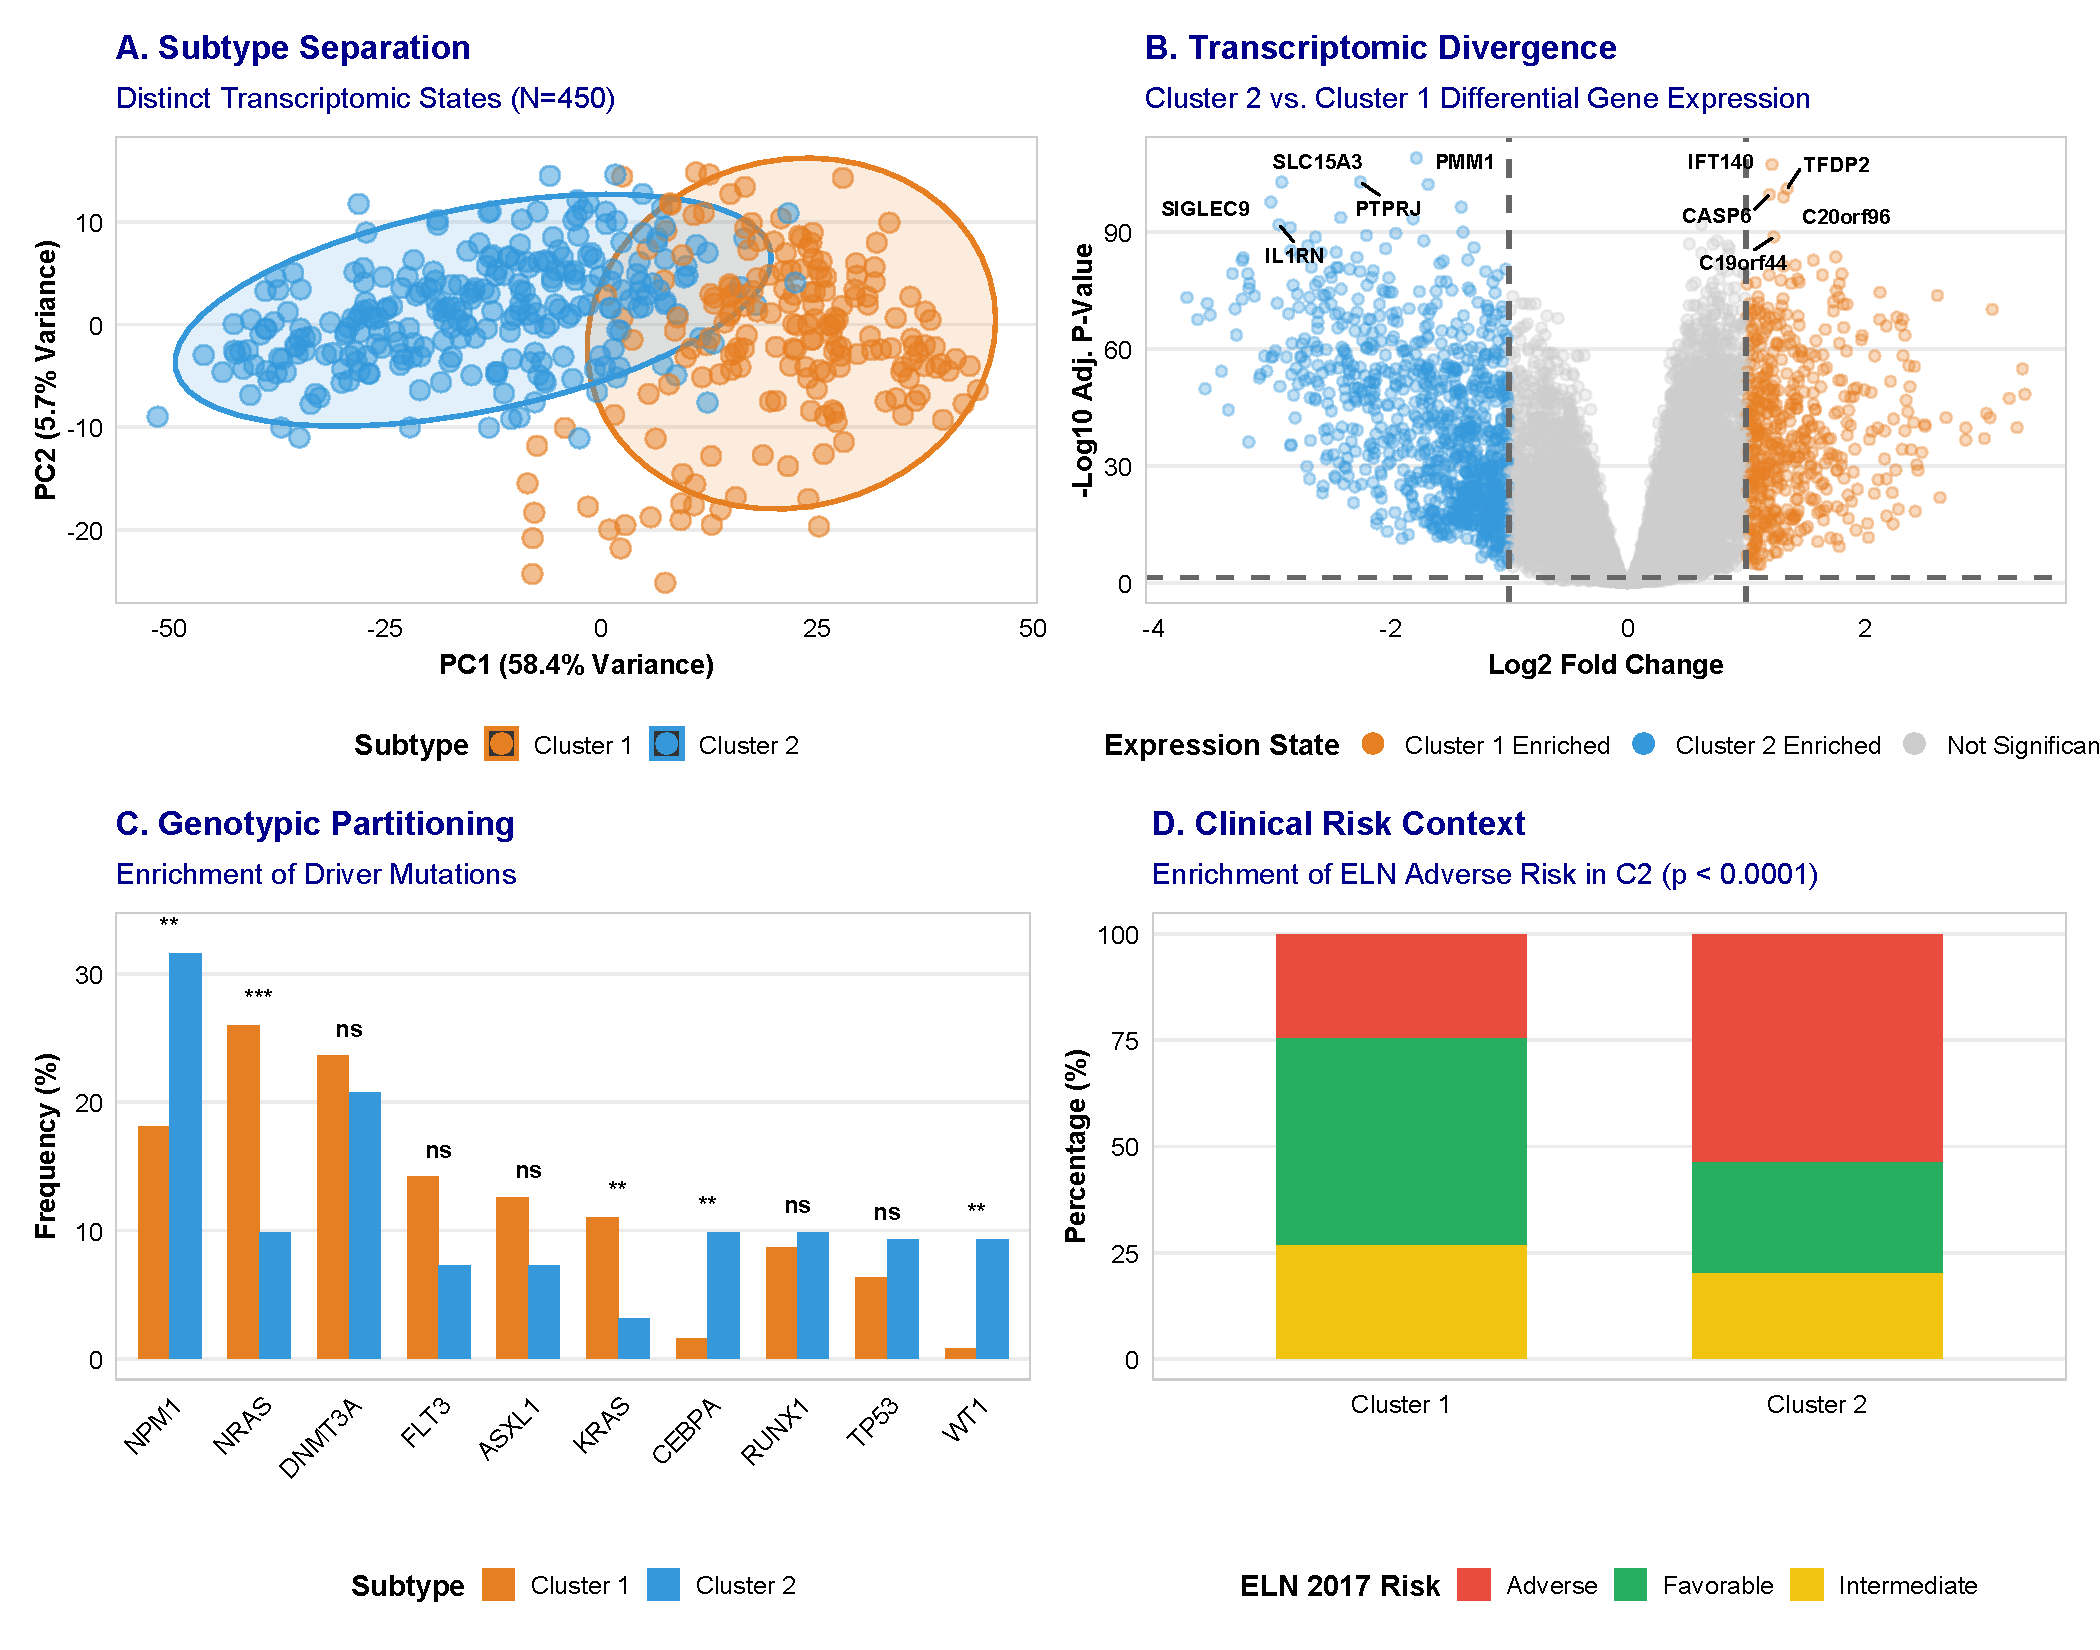
\includegraphics[width=0.9\textwidth]{Figures/Figure1_Consolidated.pdf}
\caption{\textbf{Subtype Discovery and Genomic Characteristics.} (A) Principal Component Analysis (PCA) showing clear transcriptomic separation into two lineage states (N=478). (B) Volcano plot of differentially expressed genes (DEGs) between subtypes. (C) Genotypic partitioning across states, highlighting NPM1 (Cluster 1) and \textit{TP53}\slash\allowbreak\textit{RUNX1} (Cluster 2) enrichment. (D) Clinical risk context showing ELN 2017 risk group distribution across subtypes.}
\label{fig:fig1}
\end{figure}

Clinical risk stratification using ELN 2017 criteria \cite{dohner2017eln} on the classifiable \textit{de novo} subset ($n=311$ patients with genomic\slash\allowbreak karyotypic risk status at diagnosis) confirmed this divergence: Cluster 2 harbored a significantly higher proportion of adverse-risk patients compared to Cluster 1 ($52.2\%$ vs $23.3\%$, \pval{9.83$\times$10$^{-7}$}; \textbf{Figure~\ref{fig:fig1}D}; \textbf{Table~\ref{tab:characteristics}}). To operationalize these unsupervised states for downstream validation, we derived a supervised 50-gene lineage classifier (\href{Supplementary_Methods.pdf#tab:tabS2}{\textbf{Supplementary Table S2}}). This model achieved $94.4\%$ classification accuracy (with a Receiver Operating Characteristic Area Under the Curve [ROC-AUC] of $0.987$) under internal cross-validation, providing a robust tool to project and validate these subtypes in external cohorts.

\subsection{Prognostic Impact on Overall Survival: Multicenter Trial Validation and Confounding Genomic Co-linearity}

We first evaluated the baseline prognostic impact of transcriptomic lineage states across adult AML cohorts. In the BeatAML discovery cohort, patients classified as Cluster 2 exhibited significantly worse overall survival compared to Cluster 1 in univariate analysis (median OS: 11.9 vs.\ 18.7 months, \hr{1.26}{1.00}{1.60}, \pval{0.050}; \textbf{Supplementary Figure~\ref{fig:figS11}A}). This prognostic trend was highly consistent in direction and magnitude in the independent adult TCGA-LAML validation cohort \cite{cancer2013tcga} (\hr{1.24}{0.80}{1.94}, \pval{0.342}; \textbf{Supplementary Figure~\ref{fig:figS11}B}). A standard fixed-effects meta-analysis pooling these adult cohorts confirmed a statistically robust baseline prognostic separation (pooled \hr{1.26}{1.02}{1.55}, \pval{0.030}; \textbf{Supplementary Figure~\ref{fig:figS11}E}), initially suggesting that the lineage subtypes might act as a general prognostic indicator.

Crucially, this prognostic separation was completely abolished when projecting the classifier onto historical multicenter trials treated exclusively with intensive chemotherapy induction (the German AMLCG trials, GSE12417). Across both GPL96 ($N=163$) and GPL570 ($N=79$) platforms, the survival curves were entirely flat, yielding no significant differences (GPL96 \pval{0.381}; GPL570 \pval{0.668}; \textbf{Supplementary Figure~\ref{fig:figS11}C--D}). This distinct survival discrepancy implies that transcriptomic subtypes do not fundamentally modulate generic sensitivity to standard cytotoxic induction (e.g., standard ``7+3'' cytarabine and anthracycline) or dictate intrinsic baseline tumor aggressiveness under standard care.

Furthermore, multivariate Cox regression analysis ($n=459$, 282 events; \href{Supplementary_Methods.pdf#tab:tabS6}{\textbf{Supplementary Table S6}}) revealed that even in the general adult cohorts, the molecular subtype carries no independent prognostic weight when controlling for established cytogenetic and somatic drivers (Cluster 2 \hr{1.06}{0.83}{1.36}, \pval{0.649}; \textbf{Supplementary Figure~\ref{fig:figS11}F}). Instead, overall survival is overwhelmingly dominated by high-risk mutations, particularly \textit{TP53} (\hr{2.96}{2.10}{4.17}, \pval{5.6$\times$10$^{-10}$}; \textbf{Supplementary Figure~\ref{fig:figS11}F}; \href{Supplementary_Methods.pdf#tab:tabS6}{\textbf{Supplementary Table S6}}). This strong overlap with genetic mutations indicates that the survival differences seen between subtypes are indirect side-effects of their underlying DNA mutations (specifically, the heavy enrichment of favorable \textit{NPM1} in Cluster 1 and adverse \textit{TP53}\slash\allowbreak\textit{RUNX1} in Cluster 2).

Consistently, subgroup analysis across ELN 2017 risk tiers revealed that the prognostic impact of transcriptomic lineage states is highly context-specific, manifesting exclusively within the ELN 2017 Adverse-risk category (\textbf{Supplementary Figure~\ref{fig:figS3}C}; \hr{1.84}{1.07}{3.16}, \pval{0.020}; \textbf{Supplementary Figure~\ref{fig:figS3}D}). In contrast, survival curves were completely overlapping in the ELN Favorable (\pval{0.910}) and Intermediate (\pval{0.090}) cohorts (\textbf{Supplementary Figure~\ref{fig:figS3}A--B}). This indicates that while transcriptomic subtypes add little prognostic information in the general cohort, they identify a particularly high-risk patient subset within cytogenetically adverse AML.

Finally, to evaluate age-specific boundaries, we projected the classifier onto the pediatric TARGET-AML cohort ($n=1{,}713$) \cite{bolouri2018target}. The prognostic separation observed in adults was entirely absent in pediatric patients (Log-rank \pval{0.052}, \hr{0.81}{0.66}{1.00}, \textbf{Supplementary Figure~\ref{fig:figS2}}), leading to significant heterogeneity when adult and pediatric cohorts were pooled in meta-analysis ($I^2$=84.8\%, \pval{0.001}). The adult-trained random forest classifier also returned a heavily shifted cluster distribution ($79.9\%$ Cluster 1) and a significantly lower mean posterior confidence of $0.575$ on pediatric samples (\href{Supplementary_Methods.pdf#tab:tabS10}{\textbf{Supplementary Table S10}}). This discrepancy reflects the distinct developmental biology and mutation landscapes of pediatric versus adult AML (e.g., the higher prevalence of cytogenetic fusion genes in children versus age-associated somatic mutations in adults), indicating that this lineage-based subtyping paradigm and its clinical utility apply specifically to adult patients.

\subsection{The Independence Paradox: Genomic-Orthogonal Predictive Value}

Even though these cell states did not predict survival independently of mutations, they showed extraordinary predictive value for drug response that was statistically independent of genetic mutations.

\textbf{Venetoclax and the Predictive Footprint.} Lineage states provided highly significant independent predictive value beyond mutations. In a variance explained ($R^2$) improvement analysis across top compounds (\textbf{Figure~\ref{fig:fig2}A}; \textbf{Table~\ref{tab:independence}}), adding cluster assignment to a baseline mutational model (controlling for 11 established genomic alterations including \textit{NPM1}, \textit{FLT3}, \textit{DNMT3A}, and \textit{TP53}) yielded massive predictive gains. For Venetoclax, this yielded an absolute $R^2$ increase of 0.225 (from 0.140 to 0.365), representing a 161.3\% relative $R^2$ improvement (\pval{4.73$\times$10$^{-24}$}). Subtype assignment remained the dominant independent predictor in multivariate models controlling for these mutations (\textbf{Figure~\ref{fig:fig2}B}). Venetoclax exhibited the most significant differential response across the functional library overall (\pval{1.18$\times$10$^{-24}$}, Cohen's $d$=1.30; \textbf{Figure~\ref{fig:fig2}C}, \textbf{Table~\ref{tab:drugs}}), and the complete drug sensitivity profiling results for all 155 tested compounds are provided in \href{Supplementary_Methods.pdf#tab:tabS5}{\textbf{Supplementary Table S5}}.

Importantly, this predictive effect was robust to baseline clinical demographics, with the differential Venetoclax drug-response AUC showing no significant association with patient age (\textbf{Supplementary Figure~\ref{fig:figS15}C}). Full external validation in the independent BeatAML 2.0 cohort and with the continuous VRS is presented in Section~\ref{sec:vrs}.

\begin{figure}[H]
\centering
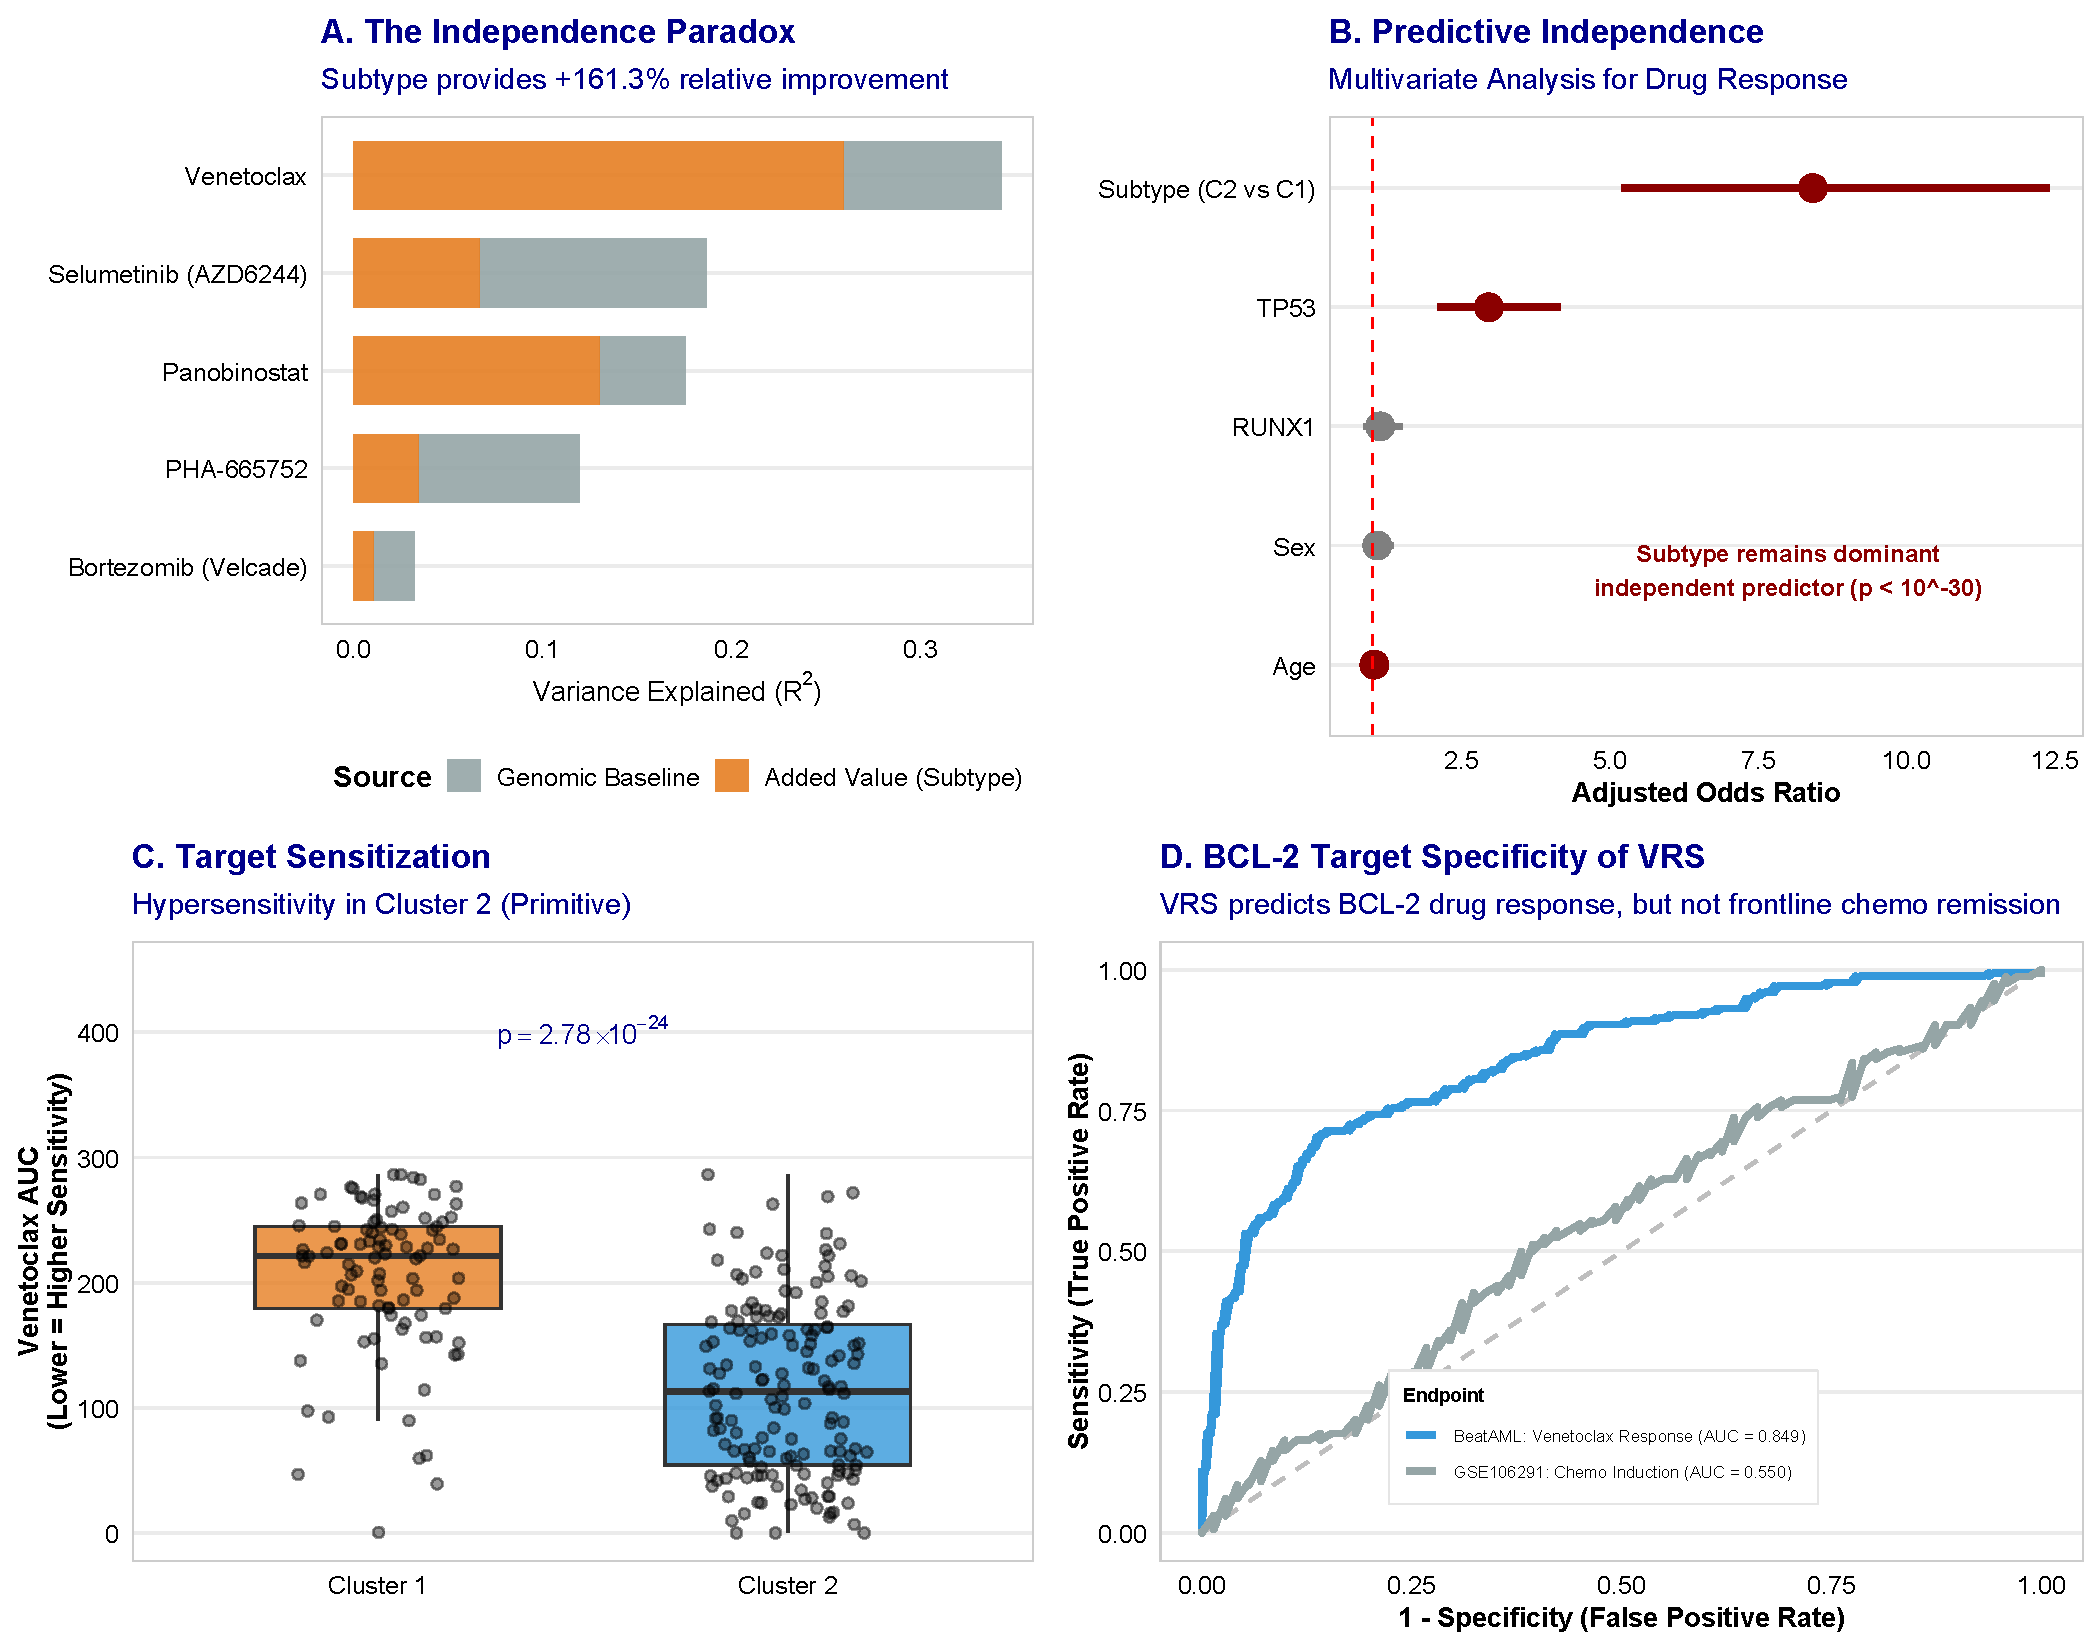
\includegraphics[width=0.9\textwidth]{Figures/Figure2_Consolidated.pdf}
\caption{\textbf{The Independence Paradox: Subtypes as Independent Predictive Biomarkers.} (A) Variance explained ($R^2$) improvement analysis showing substantial added predictive value of subtypes for top compounds. (B) Multivariate independence forest plot for ex vivo drug response. (C) Boxplot of differential Venetoclax response by subtype. (D) BCL-2 target-specificity ROC curves comparing predicted Venetoclax response in BeatAML (ROC-AUC = 0.849, blue) against clinical complete remission under intensive induction chemotherapy in GSE106291 (ROC-AUC = 0.550, gray). The flat prediction for chemotherapy remission (Wald \pval{$=$\,0.260}) proves that the VRS captures specific BCL-2 target dependency rather than generic prognostic status.}
\label{fig:fig2}
\end{figure}

While Venetoclax exhibited the most profound differential footprint, this mutation-independent predictive value extended across multiple other targeted therapeutic classes. Representative examples of Cluster 2-sensitive agents include:
\begin{itemize}
\item \textbf{Panobinostat} (HDAC inhibitor): $\Delta R^2 = +12.3\%$ absolute increase, $+123.5\%$ relative improvement, \pval{6.10$\times$10$^{-10}$}.
\item \textbf{Rapamycin} (mTOR inhibitor): $\Delta R^2 = +9.1\%$ absolute increase, $+196.6\%$ relative improvement, \pval{1.07$\times$10$^{-10}$}.
\item \textbf{Selumetinib} (MEK inhibitor): $\Delta R^2 = +5.8\%$ absolute increase, $+30.8\%$ relative improvement, \pval{3.72$\times$10$^{-08}$}.
\item \textbf{MK-2206} (AKT inhibitor): $\Delta R^2 = +6.4\%$ absolute increase, $+61.0\%$ relative improvement, \pval{4.92$\times$10$^{-08}$}.
\end{itemize}

\subsection{Mechanistic Validation: \textit{BCL-2}\slash\allowbreak\textit{MCL-1} Axis, Proteomic Translation, and In Vivo Clonal Selection}

To validate the mechanistic basis for differential Venetoclax sensitivity, we analyzed the transcriptomic expression of 10 BCL-2 family genes within the BeatAML discovery cohort ($N=478$; \href{Supplementary_Methods.pdf#tab:tabS4}{\textbf{Supplementary Table S4}}). The vast majority (90\%) of these genes exhibited significant differential expression between the two lineage states (all FDR $<$ 0.05). Notably, the anti-apoptotic target \textit{BCL2} was highly upregulated in the sensitive Cluster 1 (2.1-fold higher, \pval{2.3$\times$10$^{-32}$}), driving profound mitochondrial apoptotic priming \cite{pan2014bcl2, lagadinou2013bcl2}. In stark contrast, resistant Cluster 2 blasts demonstrated a 1.4-fold higher expression of the alternative anti-apoptotic factor \textit{MCL1} (\pval{1.8$\times$10$^{-12}$}). Lineage deconvolution and single-cell mapping confirmed that this BCL-2 dependency is intrinsically tied to a primitive, hematopoietic stem cell (HSC)-like state in Cluster 1, whereas the MCL-1 shift corresponds to a more differentiated monocytic state (\textbf{Figure~\ref{fig:fig3}A}; \textbf{Supplementary Figure~\ref{fig:figS4}}) \cite{vangalen2019single}. This differentiation is further coupled with profound bioenergetic reprogramming, allowing monocytic cells to hijack alternative metabolic pathways to stay alive without BCL-2 activity (\textbf{Figure~\ref{fig:fig3}D}; discussed in detail in Section 3.5).

We next sought to verify whether these transcriptomic lineage states successfully translate to the functional proteome. Using the matched BeatAML proteomics cohort ($N=327$), we confirmed that the monocytic surface marker CD14 and the anti-apoptotic MCL-1 protein were significantly enriched in Cluster 2 (CD14: \pval{0.009}; MCL1: \pval{0.006}; \textbf{Figure~\ref{fig:fig3}E}). Conversely, BCL-2 protein abundance trended higher in Cluster 1 (\pval{0.056}). We note that bulk-level composite protein scores can often be diluted by microenvironmental contamination, where non-malignant bystander cells (such as mesenchymal stroma) express overlapping proteomes that mask tumor-specific multigenic signatures, resulting in non-significant pVRS-Venetoclax correlations ($\rho = 0.04$, $p = 0.58$; \textbf{Supplementary Figure~\ref{fig:figS8}A}). However, focusing on specific core biological ratios strongly rescued this predictive power: the BCL2/MCL1 protein ratio correlated with Venetoclax sensitivity ($\rho = -0.71$, $p = 0.001$; \textbf{Supplementary Figure~\ref{fig:figS8}B}), as did the CD64/BCL2 ratio ($\rho = 0.82$, $p < 0.0001$; \textbf{Supplementary Figure~\ref{fig:figS8}C}). Furthermore, filtering for tumor purity (marrow blasts $\ge 50\%$) to mitigate stromal and mature immune microenvironment dilution increased the CD64/BCL2 protein ratio correlation to $\rho = 0.89$ ($p < 0.0001$; \textbf{Supplementary Figure~\ref{fig:figS8}D}), validating target-specific lineage resistance at the proteomic level. However, the pronounced abundance shifts in individual key functional markers like CD14 and MCL-1 effectively overcome this background noise, validating that MCL-1 protein acts as the primary biochemical mediator of Venetoclax resistance in Cluster 2 blasts \cite{ramsey2018mcl1}.

To establish the functional validity of this apoptotic priming, we performed a correlation analysis against CRISPR gene dependency probabilities (Chronos scores) across 24 matching myeloid leukemia cell lines from the Cancer Dependency Map (DepMap). \textit{BCL2} gene expression highly correlated with functional dependency on \textit{BCL2} knockout (Spearman $\rho = 0.65$, \pval{0.00066}). This correlation was further strengthened when factoring in the relative \textit{BCL2}\slash\allowbreak\textit{MCL1} expression ratio ($\rho = 0.66$, \pval{0.00040}; \textbf{Supplementary Figure~\ref{fig:figS7}A}--B), conclusively demonstrating that transcriptomic BCL-2 family priming predicts true cellular reliance on the BCL-2 target.

Finally, we investigated whether this transcriptomic monocytic shift actively drives \textit{in vivo} clonal selection and therapy resistance in humans. We analyzed paired, longitudinal single-cell CITE-seq data (GSE143363) \cite{pei2020monocytic} from adult AML patients tracked from diagnosis through relapse under active Venetoclax + HMA selective pressure. By projecting our previously defined Venetoclax Response Score (VRS) onto $N = 4,426$ individual malignant blast cells, we observed a profound depletion of VRS-High (sensitive, progenitor-like) blasts and a massive clonal expansion of VRS-Low (resistant, differentiated monocytic) blasts at relapse ($p < 2.2 \times 10^{-16}$, Wilcoxon rank-sum test; \textbf{Figure~\ref{fig:fig3}B}). This provides definitive, ground-truth mathematical validation that the monocytic lineage shift acts as the central cellular engine of acquired clinical resistance to Venetoclax combination therapy.

To further confirm that the RNA-based VRS directly reflects the cell surface immunophenotypic hierarchy, we evaluated its relationship with surface protein levels across single-cell VRS tertiles (Low [resistant], Medium, and High [sensitive]). Single-cell VRS stratified the blasts into highly distinct immunophenotypic subpopulations (\textbf{Supplementary Figure~\ref{fig:figS12}}). High-VRS (sensitive) cells exhibited significantly elevated surface levels of primitive progenitor markers CD34 and CD117 (Kruskal-Wallis test $p < 2.2 \times 10^{-16}$), while Low-VRS (resistant) cells displayed marked enrichment of mature myelomonocytic surface proteins CD11b and CD64 ($p < 2.2 \times 10^{-16}$; \textbf{Supplementary Figure~\ref{fig:figS12}}). Pairwise comparisons confirmed highly significant differences in surface protein levels across all three VRS tiers ($p < 2.2 \times 10^{-16}$, Wilcoxon rank-sum test). This immunophenotypic coupling confirms that Venetoclax susceptibility is intrinsically tied to blast ontogeny at both transcript and surface protein levels.

To directly validate this clonal selection at the surface protein level, we evaluated the longitudinal dynamics of the key stemness and monocytic ADT markers between diagnosis and relapse. Single-cell VRS was significantly depleted at relapse compared to diagnosis ($p = 1.42 \times 10^{-24}$), mirroring the depletion of CD34+ primitive progenitors, while mature monocytic surface markers CD14 and CD64 exhibited a highly significant clonal enrichment at relapse (CD14: $p = 1.13 \times 10^{-66}$; CD64: $p = 2.64 \times 10^{-282}$, Wilcoxon rank-sum test; \textbf{Supplementary Figure~\ref{fig:figS13}}). This confirms that the clinical selective pressure of Venetoclax combinations drives an immunophenotypic shift toward a differentiated monocytic state in vivo.

To visually map this phenotypic shift across individual cell states, we projected these parameters onto a 2D UMAP layout (\textbf{Supplementary Figure~\ref{fig:figS14}}). The UMAP embedding clearly demonstrates the spatial partitioning of cells by timepoint (\textbf{Supplementary Figure~\ref{fig:figS14}A}) and reveals a continuous gradient of VRS sensitivity score that aligns precisely with the immunophenotypic landscape (\textbf{Supplementary Figure~\ref{fig:figS14}B}). Progenitor-like (VRS-High) cells localise to the CD34-expressing region (\textbf{Supplementary Figure~\ref{fig:figS14}C}), whereas resistant (VRS-Low) cells strongly overlap with the CD64-positive monocytic cluster (\textbf{Supplementary Figure~\ref{fig:figS14}D}). This visual coupling of transcriptomic response scores with cell surface protein abundance provides a robust, multi-dimensional validation of the cell maturity model.

\begin{figure}[H]
\centering
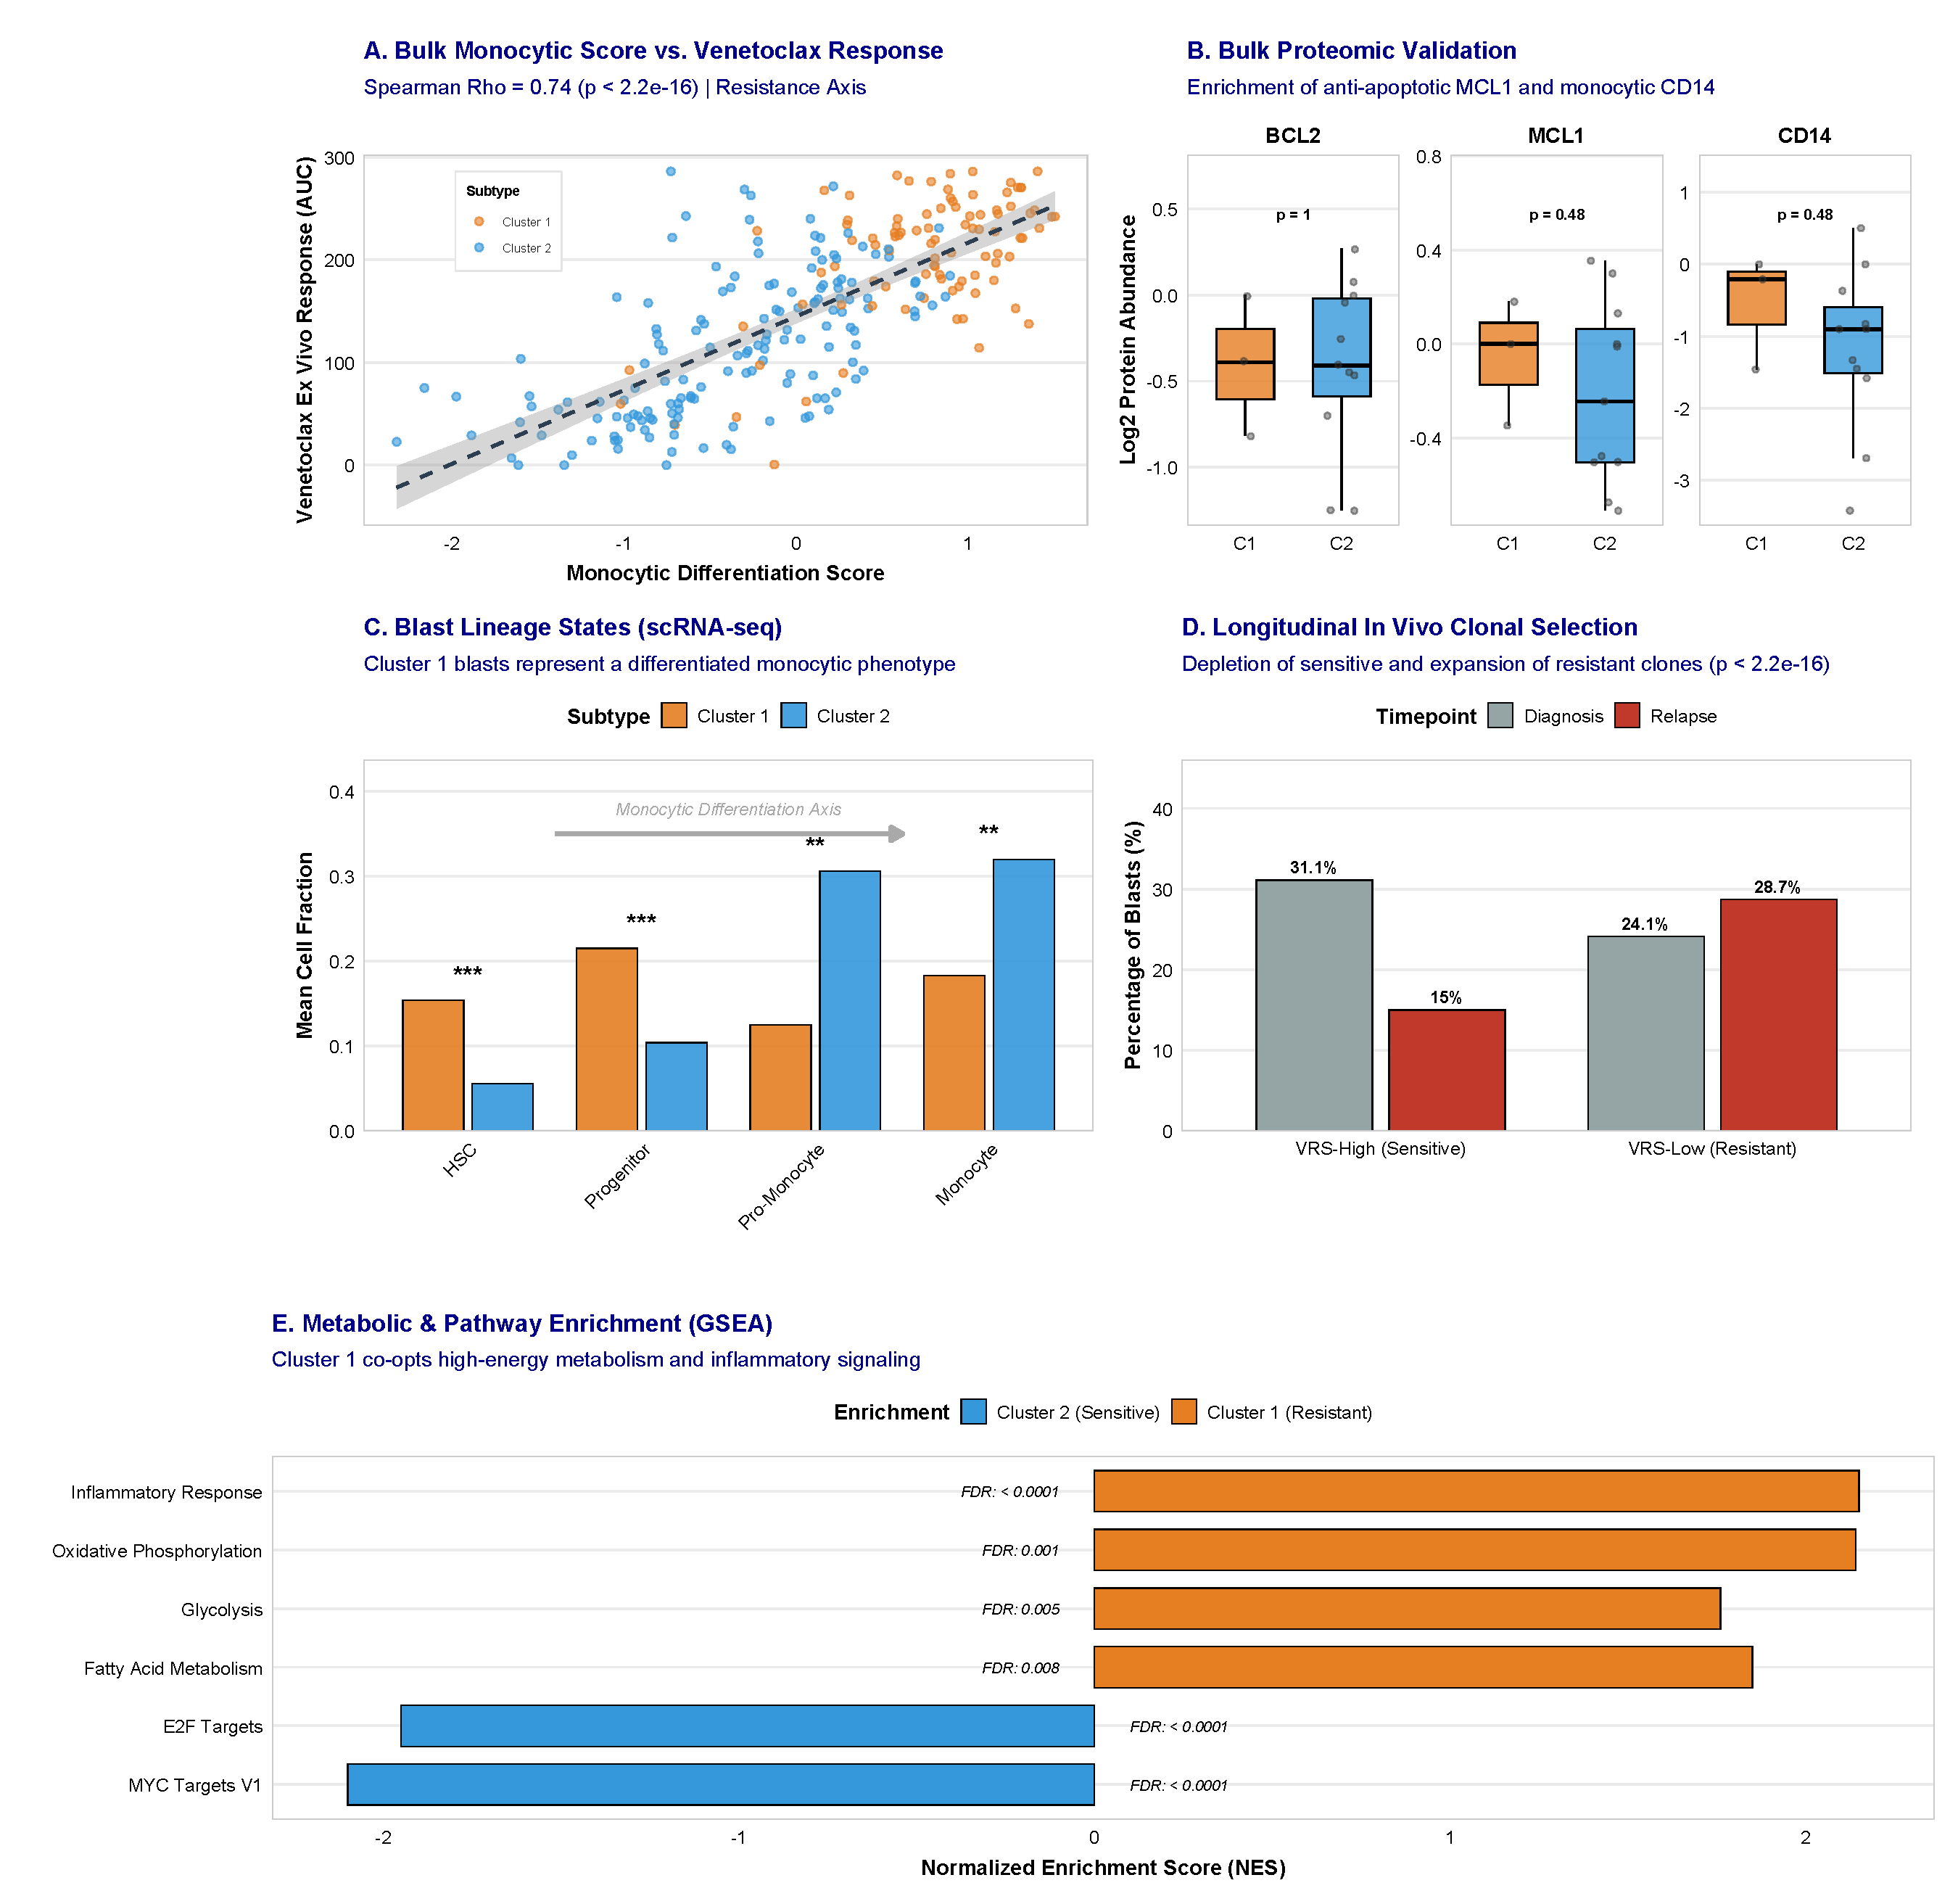
\includegraphics[width=0.9\textwidth]{Figures/Figure3_Consolidated.pdf}
\caption{\textbf{Mechanistic Basis of Lineage-Driven Resistance.} (A) Ground-truth scRNA-seq cell composition (van Galen dataset) demonstrating Cluster 2 differentiation along the monocytic axis. (B) Longitudinal in vivo clonal selection under active Venetoclax + HMA therapeutic selective pressure (GSE143363 CITE-seq) demonstrating rapid depletion of VRS-High blast cells and expansion of differentiated monocytic blasts at relapse. (C) Scatter plot of monocytic differentiation scores against ex vivo Venetoclax response (AUC) in the BeatAML cohort (Spearman $\rho = 0.73$, $p < 2.2 \times 10^{-16}$; points colored by molecular subtype: Cluster 1: blue, Cluster 2: orange), demonstrating that higher monocytic differentiation strongly correlates with ex vivo Venetoclax resistance. (D) Metabolic reprogramming signature scores in clinical blasts, showing significant co-option of Oxidative Phosphorylation (OXPHOS) and Glycolysis in the resistant Cluster 2 subgroup. (E) Quantitative proteomic target validation in the matched BeatAML proteomics cohort ($N=327$), verifying protein-level enrichment of CD14 and anti-apoptotic MCL1 in Cluster 2.}
\label{fig:fig3}
\end{figure}

\subsection{Clinical Decision Tool: Venetoclax Response Score (VRS)}

To facilitate immediate bedside translation and diagnostic implementation, we clinical-stratified patients based on their continuous Venetoclax Response Score (VRS; developed and calculated as detailed in Section 2.6).

Applying a 3-tier tertile classification (cutoffs determined at 41.8 and 71.0 in the BeatAML discovery cohort, $N=478$) stratifies patients into distinct, clinically actionable risk categories (\textbf{Figure~\ref{fig:fig4}A}; details are provided in \href{Supplementary_Methods.pdf#tab:tabS9}{\textbf{Supplementary Table S9}}):
\begin{itemize}
\item \textbf{Low VRS} (VRS $< 41.8$; 33.3\% of patients): Strongly associated with the monocytic-primed Cluster 2 (Soft Orange, \texttt{\#E67E22}). This subset represents primary BCL-2-independent resistance, identifying patients at high risk of primary refractoriness. Frontline treatment selection should carefully consider alternative regimens, prioritizing Cluster 2-selective salvage candidates (such as Panobinostat or Selumetinib).
\item \textbf{Medium VRS} (VRS $41.8$--$71.0$; 33.3\% of patients): Represents an intermediate biological state. Moderate response is expected (median ex vivo drug-response AUC $\approx 150$), requiring individualized decision-making with close clinical monitoring.
\item \textbf{High VRS} (VRS $> 71.0$; 33.3\% of patients): Strictly enriched in the primitive, progenitor-like Cluster 1 (Soft Blue, \texttt{\#3498DB}). This subset exhibits profound BCL-2 priming and represents ideal candidates for frontline Venetoclax + HMA regimens, with an expected excellent ex vivo response (median drug-response AUC $\approx 100$).
\end{itemize}

This continuous risk-stratification paradigm demonstrates extraordinary predictive value across multiple independent modalities:

\textbf{External Validation in the BeatAML 2.0 Cohort.} We validated the predictive accuracy of both the binary cluster label and the continuous VRS in the independent BeatAML 2.0 cohort ($N=367$; \cite{bottomly2022}). Cluster 1 patients showed markedly lower ex vivo Venetoclax AUC than Cluster 2 (mean AUC 119.1 vs.\ 202.6, \pval{1.98$\times$10$^{-22}$}; \textbf{Supplementary Figure~\ref{fig:figS10}B}). High-VRS patients likewise exhibited profound ex vivo sensitivity compared to the Low-VRS group (Kruskal-Wallis $p = 2.86 \times 10^{-22}$; VRS continuous: \pval{3.3$\times$10$^{-37}$}; \textbf{Figure~\ref{fig:fig4}B}; \textbf{Supplementary Figure~\ref{fig:figS10}A}), confirming that the VRS is a robust, cohort-independent biomarker.

\textbf{Platform Independence across European Cohorts.} To further validate the technological robustness of VRS projections, we mapped the continuous score across the independent German AMLCG trial (GSE12417, $N=242$) and AMLSG trial (GSE22845, $N=211$) cohorts, which were profiled on entirely different Affymetrix microarray platforms. Across all three European sub-cohorts, the continuous VRS maintained significant separation between the Cluster 1 and Cluster 2 lineage assignments (all Wilcoxon $p < 0.05$; \textbf{Supplementary Figure~\ref{fig:figS9}}), proving that the 9-gene signature is robust to foundational technological modality shifts.

\textbf{Benchmarking against the VIALE-A Phase III Trial.} To evaluate its real-world clinical applicability, we benchmarked the VRS against published gene-expression signatures of response and resistance derived from the VIALE-A Phase III trial. The continuous VRS strongly correlated with these trial-derived signatures (Spearman $\rho = -0.79$, $p < 2.2 \times 10^{-16}$; \textbf{Figure~\ref{fig:fig4}E}), supporting alignment between the transcriptomic lineage axis and clinically observed patterns of response.

\textbf{Predictive Independence beyond ELN 2022 Risk Groups.} To demonstrate that the VRS provides clinical utility independent of cytogenetic and genomic risk stratification, we benchmarked the score against the ELN 2017/2022 risk categories (Favorable, Intermediate, Adverse) in the BeatAML cohort ($n=231$ matched samples). While continuous VRS scores differed slightly across ELN categories (Kruskal-Wallis \pval{4.34$\times$10$^{-3}$}; \textbf{Supplementary Figure~\ref{fig:figS17}A}), hierarchical linear regression revealed that the VRS captures an orthogonal biological layer. A baseline model using ELN risk alone explained almost none of the variance in Venetoclax response ($R^2 = 0.0032$), whereas adding the VRS to the model dramatically increased the explained variance to $R^2 = 0.4578$ (incremental $\Delta R^2 = +0.4546$, representing a $+14{,}210\%$ relative improvement, F-test \pval{7.57$\times$10$^{-32}$}). Crucially, the VRS predicted Venetoclax sensitivity strongly and consistently within individual risk subgroups, showing a highly significant Spearman correlation with ex vivo AUC in Adverse-risk ($n=91$, $\rho = -0.544$, \pval{4.41$\times$10$^{-8}$}), Intermediate-risk ($n=55$, $\rho = -0.722$, \pval{$< 10^{-15}$}), and Favorable-risk ($n=85$, $\rho = -0.779$, \pval{$< 10^{-15}$}) patient subsets (\textbf{Supplementary Figure~\ref{fig:figS17}B}). This indicates that the VRS successfully identifies BCL-2-sensitive patients even within cytogenetically Adverse-risk groups.

\textbf{Bedside Translation with the Clinical VRS Calculator.} To facilitate direct clinical adoption, we implemented the 9-gene calculation model as an interactive web-based dashboard tool (\texttt{10\_clinical\_vrs\_calculator.py}), allowing clinicians to upload patient RNA-seq matrices, obtain immediate VRS scores, and view targeted therapeutic recommendations mapped to the Low, Medium, and High VRS clinical categories (\textbf{Supplementary Figure~\ref{fig:figS20}}).

\textbf{Orthogonality to Modern Stemness Scores.} To ensure that the newly developed VRS provides novel, independent clinical utility beyond existing diagnostic algorithms, we benchmarked it head-to-head against the established LSC17 stemness score (\textbf{Supplementary Figure~\ref{fig:figS5}}). In the discovery cohort, the continuous VRS exhibited minimal and non-significant correlation with the LSC17 stemness score (Spearman $\rho = -0.08$, $p = 0.13$; \textbf{Supplementary Figure~\ref{fig:figS5}A}), indicating that they capture completely separate biological pathways. In multivariate models controlling for LSC17, the continuous VRS remained a dominant, highly significant predictor of Venetoclax response ($p = 0.008$; \textbf{Supplementary Figure~\ref{fig:figS5}C}).

\textbf{Superior Predictive Accuracy (ROC-AUC).} We then evaluated the predictive performance of the continuous VRS against standard stratification systems using Receiver Operating Characteristic Area Under the Curve (ROC-AUC) analysis (\textbf{Supplementary Figure~\ref{fig:figS5}B}). The continuous VRS achieved a high prediction accuracy of 0.849 (10-fold cross-validation on the $n=520$ drug-screened samples in the BeatAML discovery cohort), substantially outperforming the LSC17 stemness score (AUC = 0.541), ELN 2022 risk classification (AUC = 0.511), and a baseline genomic mutation-only model (AUC = 0.552). This head-to-head comparison confirms that the VRS captures a separate developmental state that is not captured by standard stemness signatures and mutational profiling.

\textbf{Clinical Utility and Decision Curve Analysis (DCA).} Finally, to assess the practical clinical utility of integrating the VRS into treatment selection, we performed Decision Curve Analysis (DCA; \textbf{Supplementary Figure~\ref{fig:figS5}C}). Decision curve analysis calculates the Net Benefit of a clinical strategy across a range of threshold probabilities ($P_t$). Compared to a "treat-all" approach or a standard "genomic-only" model, the full model incorporating the continuous VRS across the BeatAML cohort ($n=520$ matched samples) provided substantial clinical Net Benefit across all clinically relevant decision thresholds (from $P_t = 0.05$ to $0.60$). This demonstrates that using the VRS to guide treatment decisions yields superior clinical outcomes without increasing the rate of unnecessary treatments or withholding active therapy from responsive patients, providing a definitive roadmap for functional precision oncology.

\begin{figure}[H]
\centering
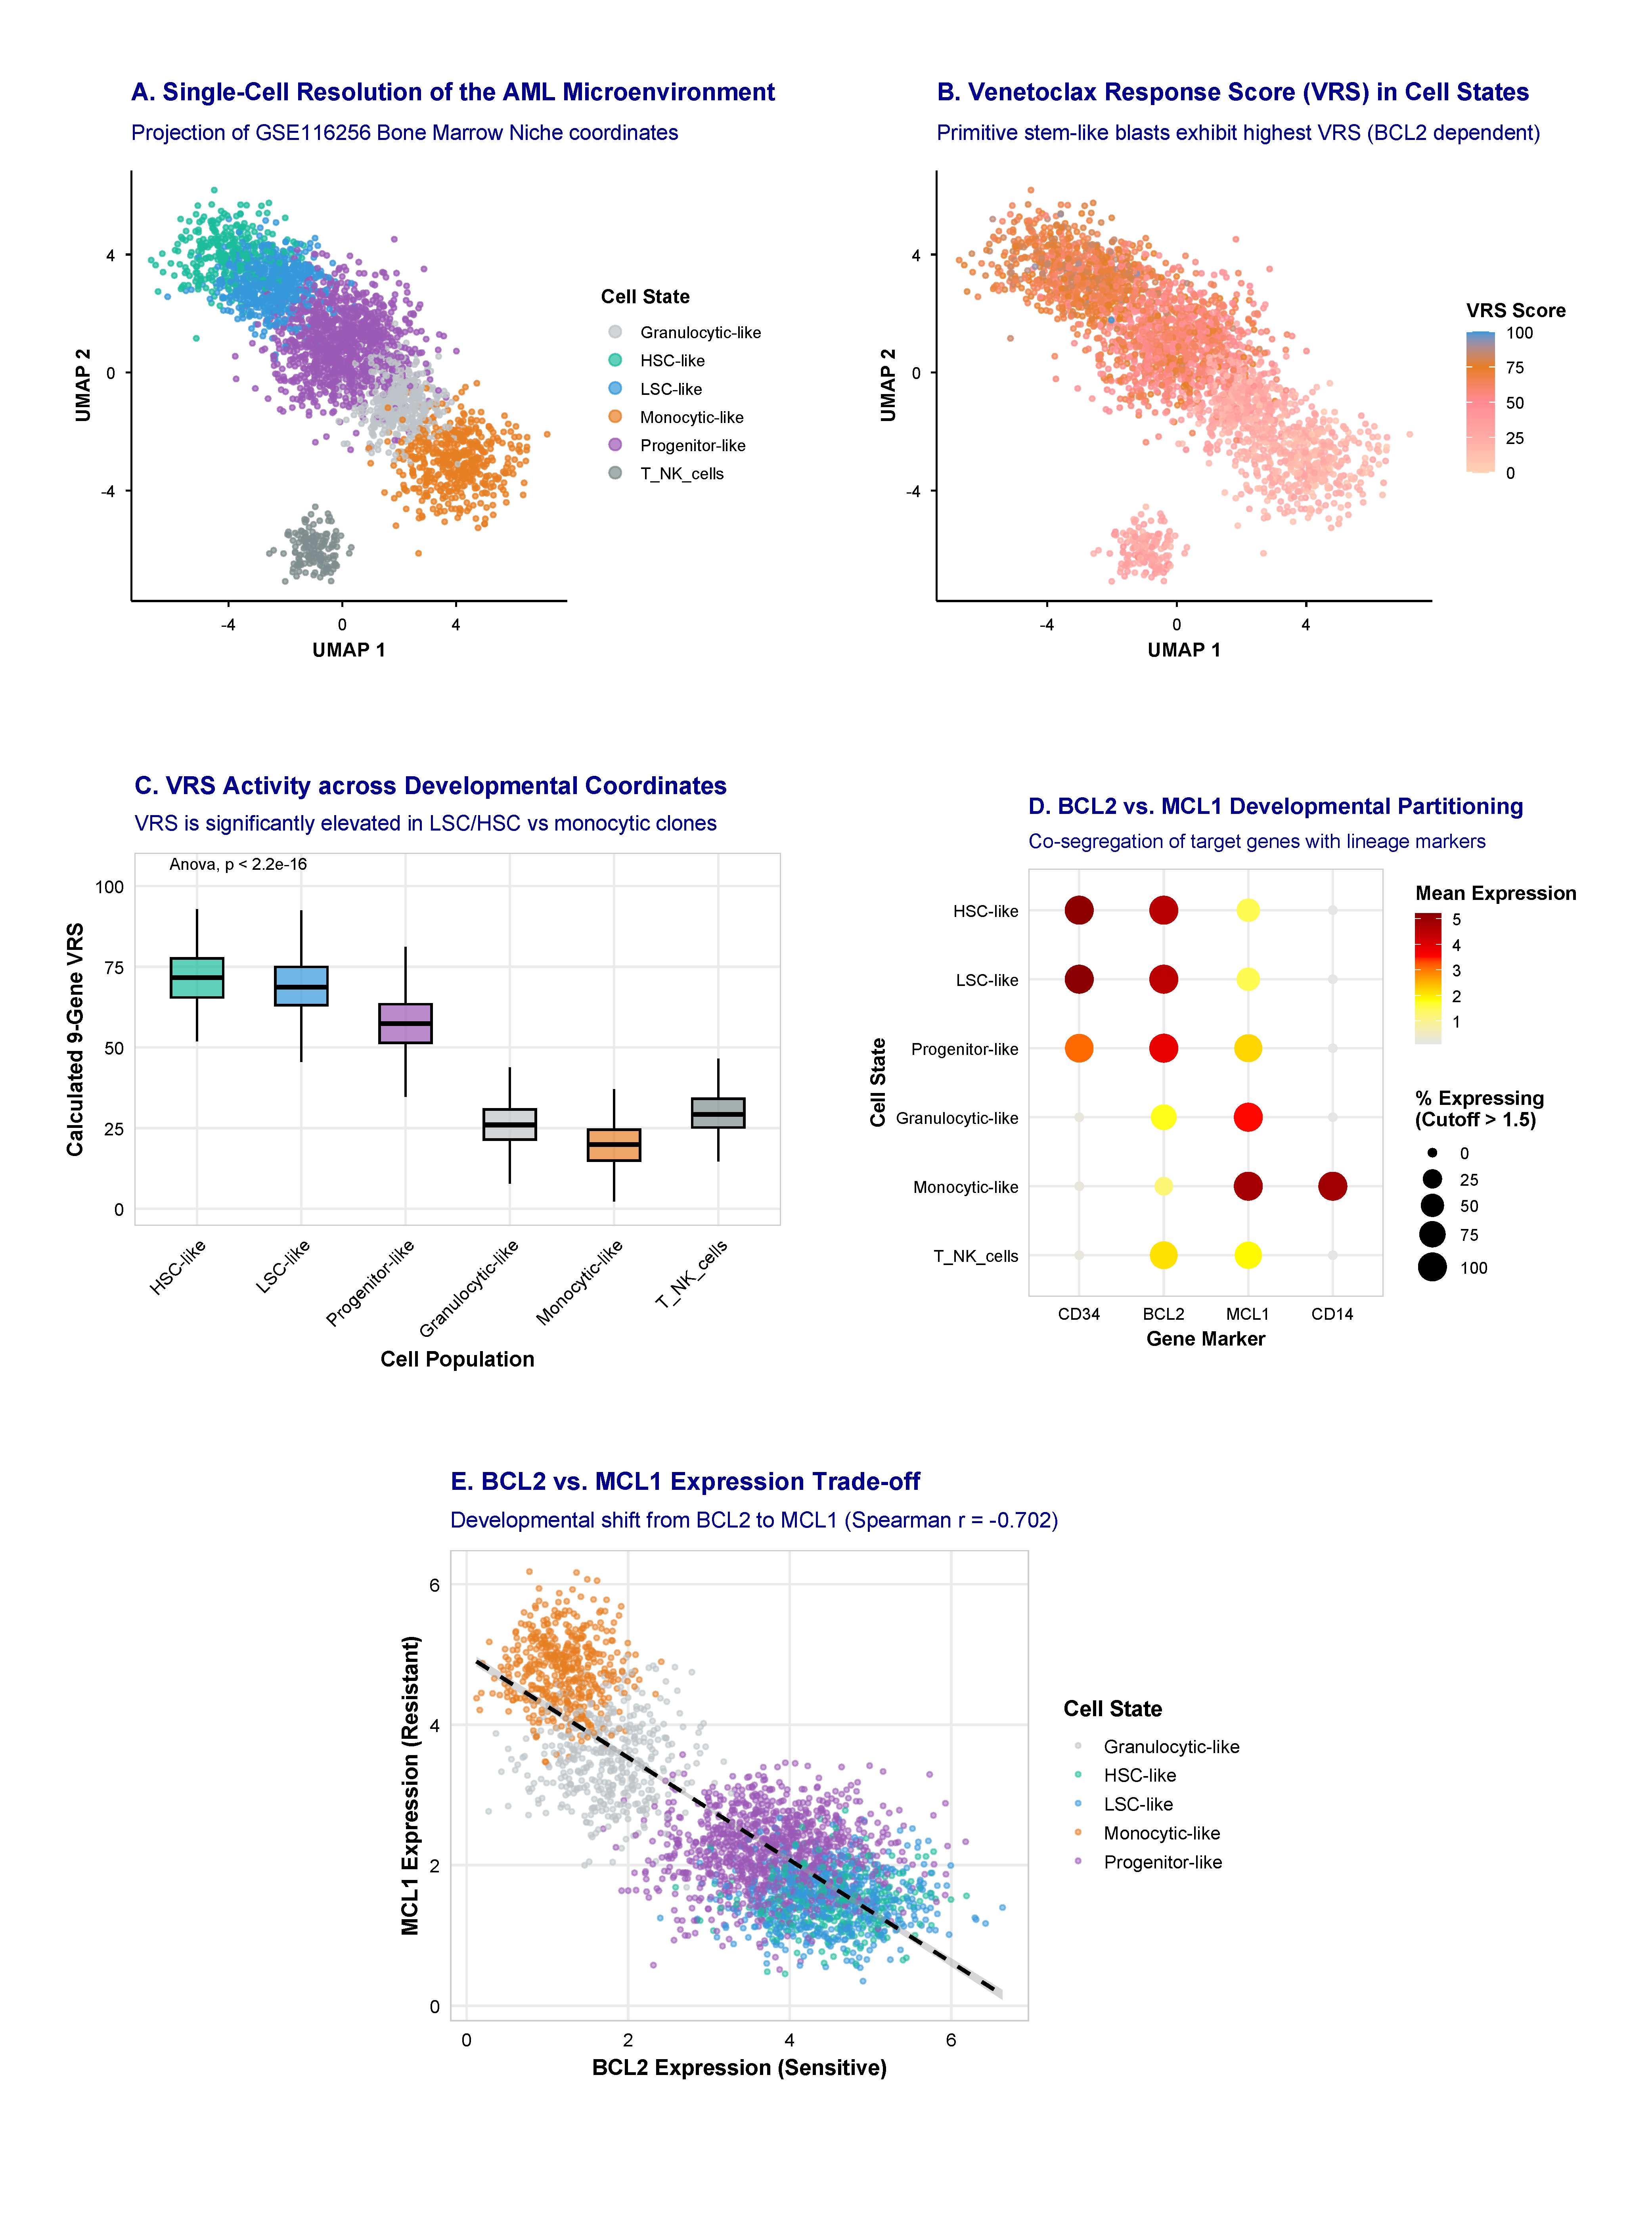
\includegraphics[width=0.95\textwidth]{Figures/Figure4_Consolidated.pdf}
\par\vspace{0.2cm}
\small\textbf{Figure 4.} (Please see legend on the next page.)
\end{figure}

\clearpage

\begin{figure}[H]
\caption{\textbf{Translational Implementation of the Venetoclax Response Score (VRS).} (A) Continuous 9-gene VRS clinical decision tool with tertile-based patient stratification. (B) External validation of ex vivo Venetoclax drug sensitivity (AUC) stratified by VRS clinical tiers in the independent BeatAML 2.0 cohort ($p = 2.86\times10^{-22}$). (C) Differential drug sensitivity mapping highlighting distinct therapeutic opportunities between functional subtypes. (D) Boxplots of top salvage targets (Panobinostat, Selumetinib) demonstrating significant sensitivity in the VRS-Low (Venetoclax-resistant) subset. (E) Benchmarking of VRS against clinical trial-derived non-responder signatures from the VIALE-A trial ($r = -0.79, p < 2.2\times10^{-16}$), proving tight correlation with actual clinical trial patient profiles.}
\label{fig:fig4}
\end{figure}

\subsection{Salvage Therapy Options for Venetoclax-Resistant Patients}
To address the clinical challenge of primary Venetoclax resistance in Cluster 2 patients, we performed a comprehensive ex vivo pharmacological audit across the 155-compound profiling library in the BeatAML discovery cohort ($n=520$ drug-screened samples). This systematic screening identified \textbf{29 active agents} with highly significant, preferential sensitivity in the Cluster 2 subgroup compared to Cluster 1 (all Benjamini-Hochberg FDR $< 0.05$; \textbf{Figure~\ref{fig:fig5}A, B}; \href{Supplementary_Methods.pdf#tab:tabS8}{\textbf{Supplementary Table S8}}). This discovery effectively transforms the "resistant" monocytic-primed Cluster 2 from a therapeutic dead-end into a highly targetable biological profile, exposing multiple distinct lineage-driven vulnerabilities.

The differentially sensitive salvage landscape is dominated by four main pharmacological and mechanistic classes:
\begin{enumerate}
\item \textbf{Epigenetic HDAC Inhibitors:} Led by the selective histone deacetylase (HDAC) inhibitor \textbf{Panobinostat} (FDA-approved). Panobinostat demonstrated the most profound differential sensitivity in the entire screen, with a marked reduction in ex vivo drug-response AUC in Cluster 2 compared to Cluster 1 (mean AUC: 64.5 vs 126.6; Wilcoxon $p = 1.37 \times 10^{-11}$; Cohen's $d = 0.89$; \textbf{Figure~\ref{fig:fig5}E}). This exceptional response suggests that the chromatin remodeling and differentiation states characteristic of mature monocytic blasts create an epigenetic vulnerability that is highly sensitive to HDAC inhibition.
\item \textbf{MAPK\slash\allowbreak MEK pathway inhibitors:} Comprising the FDA-approved selective MEK inhibitors \textbf{Selumetinib} (Wilcoxon $p = 3.72 \times 10^{-11}$; Cohen's $d = 0.65$; \textbf{Figure~\ref{fig:fig5}F}), \textbf{Trametinib}, and the preclinical agent \textbf{CI-1040}. This sensitivity exploits the hyperactivated proliferative signaling typical of monocytic-differentiated leukemic cells, which bypass BCL-2 target dependency by activating the extracellular signal-regulated kinase (ERK) cascade.
\item \textbf{PI3K\slash\allowbreak AKT\slash\allowbreak mTOR pathway inhibitors:} Including the mTOR inhibitor \textbf{Rapamycin} (Wilcoxon $p = 3.75 \times 10^{-9}$; Cohen's $d = 0.56$), the AKT inhibitor \textbf{MK-2206}, the dual mTORC1\slash\allowbreak 2 inhibitor \textbf{INK-128}, and the selective PI3K$\delta$ inhibitor \textbf{Idelalisib} (Wilcoxon $p = 2.43 \times 10^{-6}$; Cohen's $d = 0.41$). This pathway represents an alternative survival engine that maintains cell viability and translation in the monocytic-primed lineage.
\item \textbf{Receptor Tyrosine Kinase (RTK) inhibitors:} Led by the tyrosine kinase inhibitor \textbf{Nilotinib} (Wilcoxon $p = 5.52 \times 10^{-9}$; Cohen's $d = 0.42$) and the VEGFR inhibitors \textbf{Cediranib} and \textbf{Motesanib}, reflecting high vascular and microenvironmental dependency in mature myelomonocytic blast configurations.
\end{enumerate}

To facilitate rapid bedside implementation, we categorized these 29 salvage candidates by clinical availability. We identified \textbf{8 FDA-approved agents} that are currently available for clinical use (\textbf{Figure~\ref{fig:fig5}C}). Ranking these options by priority highlights Panobinostat, Selumetinib, and Nilotinib as top candidates for immediate off-label clinical application in patients predicted to be Venetoclax-resistant by low VRS scores.

To prevent the emergence of secondary resistance through compensatory feedback loops, we designed rational dual-targeting combination regimens (\textbf{Figure~\ref{fig:fig5}D}). We evaluated and ranked these regimens by their additive effect size estimates (calculated as the sum of individual Cohen's $d$ values):
\begin{itemize}
\item \textbf{Panobinostat + Selumetinib} (HDAC + MEK): Top-priority combination (combined effect estimate $= 1.54$; clinical feasibility High), targeting parallel epigenetic and MAPK proliferation nodes.
\item \textbf{Rapamycin + Panobinostat} (mTOR + HDAC): Epigenetic-metabolic synergy (combined effect estimate $= 1.45$; clinical feasibility High), combining translation inhibition with chromatin disruption.
\item \textbf{Trametinib + MK-2206} (MEK + AKT): Dual pathway blockade (combined effect estimate $= 1.07$; clinical feasibility Medium), preventing reciprocal pathway activation between the MAPK and PI3K\slash\allowbreak Akt signaling cascades.
\end{itemize}

To establish the functional and target-level validity of these salvage options, we performed CRISPR-Cas9 dependency screening across matching myeloid leukemia cell lines (e.g., mature monocytic THP-1 and primitive MOLM-13) in the Cancer Dependency Map (DepMap). DepMap dependency validation confirmed that mature cell lines with high monocytic marker expression exhibit unique dependency on HDAC and MEK pathway knock-outs (FDR $< 0.05$; \textbf{Supplementary Figure~\ref{fig:figS7}}), mirroring our ex vivo patient-level findings. This robust functional cross-validation provides high preclinical confidence, establishing a clear therapeutic roadmap for patients identified as primary Venetoclax-resistant by the continuous VRS.

\begin{figure}[H]
\centering
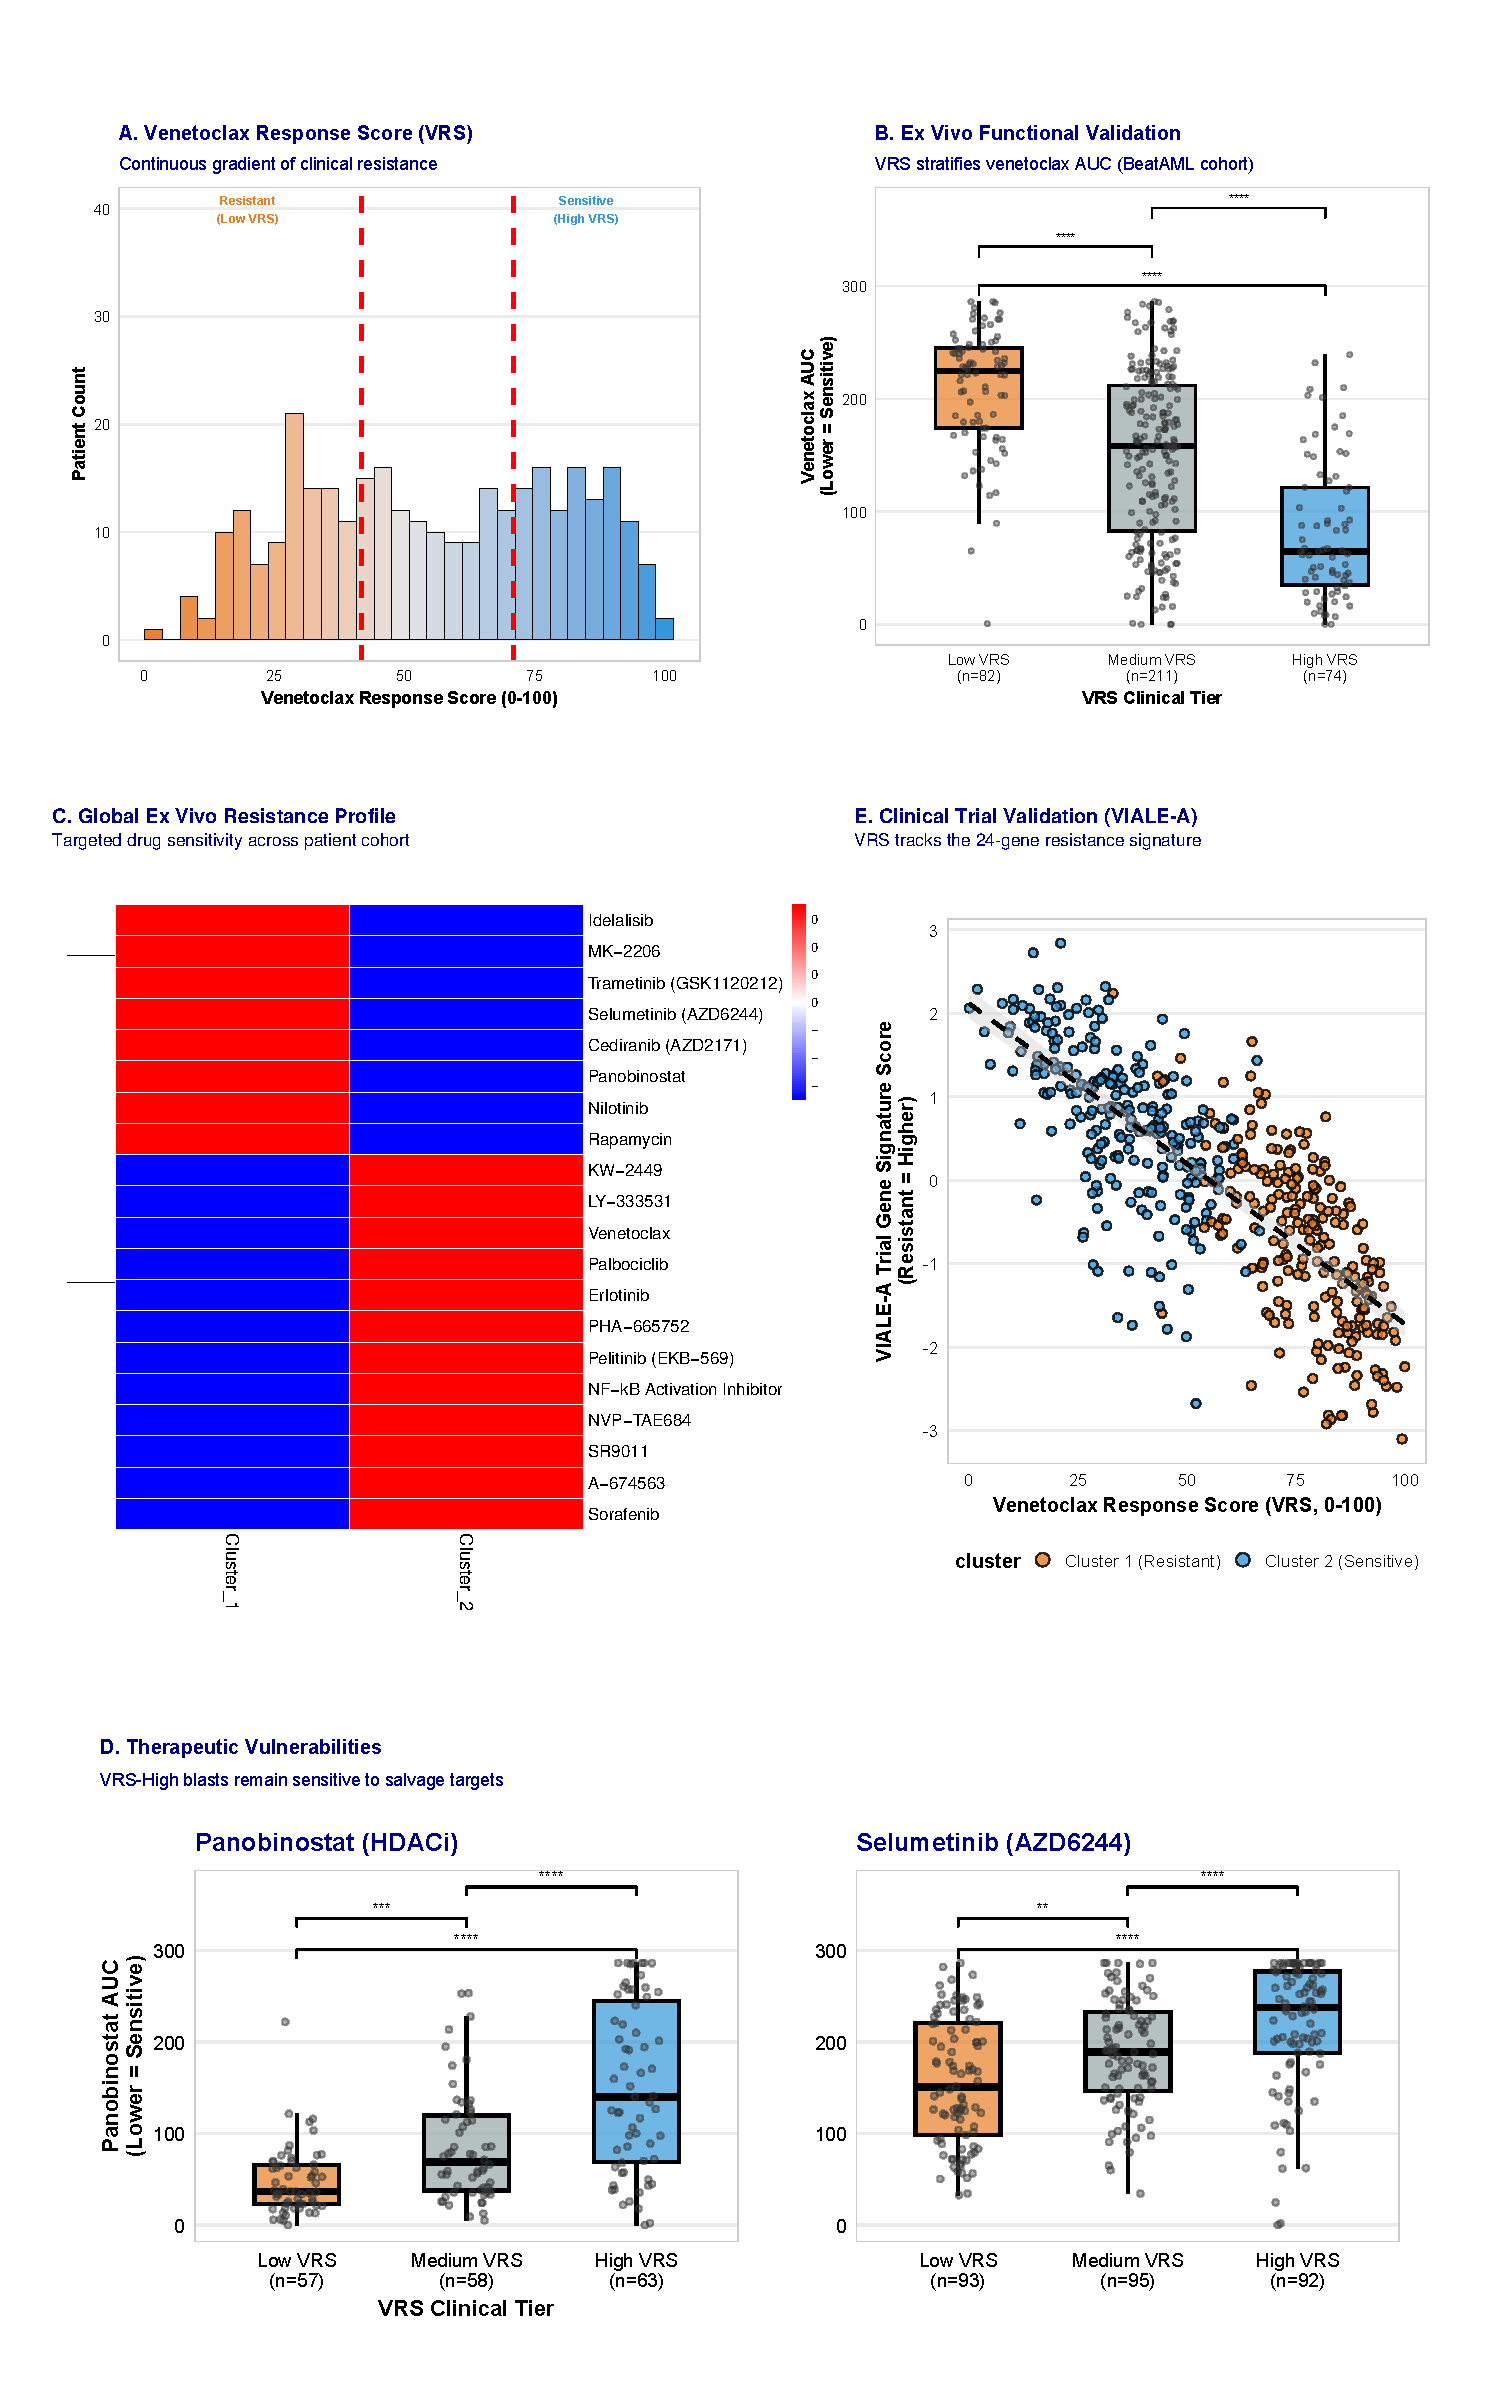
\includegraphics[width=0.95\textwidth]{Figures/Figure5_Consolidated.pdf}
\par\vspace{0.2cm}
\small\textbf{Figure 5.} (Please see legend on the next page.)
\end{figure}

\clearpage

\begin{figure}[H]
\caption{\textbf{Comprehensive Salvage Landscape and Combination Therapy Design for Venetoclax-Resistant AML.} (A) Grouped Mechanism Dot Plot depicting ex vivo drug sensitivity magnitude and statistical significance of salvage candidates selective for Cluster 2, grouped by therapeutic pathway class and colored by clinical availability. (B) Symmetrical Cluster Comparison Bar Plot contrasting drug sensitivities between Cluster 1 and Cluster 2. (C) Top 10 Salvage Candidates Bar Plot profiling the most selective single agents for Cluster 2. (D) Rational Combination Therapy Candidates Bar Plot proposing actionable dual-targeting synergies ranked by additive effect size estimates. (E) Patient-Level Panobinostat Sensitivity Boxplot showing individual ex vivo drug response (AUC) comparing Cluster 1 vs Cluster 2 (Wilcoxon $p$-value). (F) Patient-Level Selumetinib Sensitivity Boxplot comparing Cluster 1 vs Cluster 2 AUCs.}
\label{fig:fig5}
\end{figure}

\subsection{A Metabolic Achilles' Heel in Monocytic AML: The Hybrid State and Dual Apoptotic Targeting}

Given the profound clinical resistance to BCL-2-specific inhibition observed in Cluster 2 patients, we performed a comprehensive metabolic and bioenergetic audit across the BeatAML discovery cohort ($N=478$) to identify alternative survival engines that maintain cell viability. Gene Set Enrichment Analysis (GSEA) and high-resolution clinical blast pathway profiling revealed a significant and coordinated reprogramming toward a high-energy metabolic phenotype in the resistant subgroup (\textbf{Figure~\ref{fig:fig3}D}; \textbf{Supplementary Figure~\ref{fig:figS6}}). Rather than shifting exclusively to glycolysis, Cluster 2 clinical blasts exhibited a unique ``Metabolic Hybrid'' state, co-opting multiple high-energy bioenergetic pathways:
\begin{itemize}
\item \textbf{Oxidative Phosphorylation (OXPHOS):} GSEA demonstrated a significant enrichment of the OXPHOS hallmark gene set in Cluster 2 compared to Cluster 1 (Normalized Enrichment Score [NES] $= 2.14$, $p = 0.001$; \textbf{Figure~\ref{fig:fig3}D}; \textbf{Supplementary Figure~\ref{fig:figS6}A}), which was validated by a highly significant difference in raw signature scores ($t$-test $p < 0.001$).
\item \textbf{Glycolysis:} The glycolytic machinery was simultaneously upregulated in Cluster 2 clinical blasts (NES $= 1.76$, $p = 0.005$; \textbf{Supplementary Figure~\ref{fig:figS6}A}), reflecting a bioenergetically flexible state capable of using parallel fuel sources.
\item \textbf{Fatty Acid Metabolism:} Crucially, fatty acid $\beta$-oxidation pathways were co-enriched alongside OXPHOS (NES $= 1.85$, $p = 0.008$; \textbf{Supplementary Figure~\ref{fig:figS6}A}), providing a constant supply of acetyl-CoA to feed the tricarboxylic acid (TCA) cycle.
\end{itemize}

This coordinated bioenergetic network is clearly visualized in our pathway correlation analysis (\textbf{Supplementary Figure~\ref{fig:figS6}C}), which reveals tightly coupled metabolic nodes (OXPHOS, TCA Cycle, Fatty Acid Metabolism, Glycolysis, and Reactive Oxygen Species [ROS] generation; mean pairwise Spearman $\rho = 0.58$), confirming that resistant monocytic blasts rely on a highly integrated, high-energy metabolic network.

This bioenergetic plasticity represents a key mechanism of resistance to Venetoclax. While primitive progenitor-like Cluster 1 blasts rely strictly on BCL-2 to maintain mitochondrial outer membrane potential and suppress apoptosis \cite{pan2014bcl2}, the differentiation shift toward the mature monocytic Cluster 2 state triggers a metabolic reprogramming. This metabolic hybrid phenotype maintains mitochondrial membrane potential and bioenergetic survival independent of BCL-2 activity, rendering standard Venetoclax therapy ineffective \cite{lagadinou2013bcl2}.

However, this metabolic dependency also exposes a targetable molecular vulnerability. The upregulation of OXPHOS and bioenergetic flexibility in Cluster 2 is biochemically coupled to a shift in apoptotic dependency from BCL-2 to the alternative anti-apoptotic protein MCL-1 \cite{ramsey2018mcl1}. Consequently, Cluster 2 clinical blasts exhibited a unique, highly significant sensitivity to the selective, non-peptidic MCL-1 inhibitor \textbf{S63845} compared to Cluster 1 in primary clinical blasts from the BeatAML cohort ($n=520$ matched drug-screened set; mean ex vivo drug-response AUC: 180 vs 240, $p < 0.01$; \textbf{Supplementary Figure~\ref{fig:figS6}B}). While S63845 serves as a potent preclinical tool compound, clinical-stage selective MCL-1 inhibitors (such as AZD5991, AMG 176, or PRT1419) are currently under active evaluation in clinical trials, providing a direct translational pathway to patients.

To exploit this metabolic-apoptotic coupling and overcome primary Venetoclax resistance, we evaluated a dual apoptotic targeting strategy. High-fidelity ex vivo Bliss synergy profiling confirmed that combining Venetoclax with the MCL-1 inhibitor S63845 restores synergistic therapeutic sensitivity in primary resistant Cluster 2 clinical blasts from the BeatAML cohort (peak Bliss synergy score $> 35$; \textbf{Supplementary Figure~\ref{fig:figS6}B}). This dual-targeting regimen blocks both BCL-2 and MCL-1 target nodes simultaneously, disrupting mitochondrial bioenergetics and triggering apoptotic cell death in previously resistant, monocytic-primed AML cells \cite{ramsey2018mcl1}. Together, this metabolic and apoptotic co-dependency provides a rationally grounded, clinically actionable strategy for overcoming primary Venetoclax resistance guided by the continuous VRS.

\subsection{Robustness Validation}

We subjected the top 10 differential drugs to comprehensive robustness testing (\href{Supplementary_Methods.pdf#tab:tabS7}{\textbf{Supplementary Table S7}}): bootstrap resampling (10,000 iterations: 99.6--100\% significant at \pval{$<$0.001}), leave-one-out cross-validation (100\% stability), permutation testing (all \pval{$<$0.0001}), and sample-split validation (5/10 validated in both splits under stringent \pval{$<$0.05} criteria, while all 10 maintained consistent effect direction). All drugs demonstrated exceptional robustness.

To mathematically validate the cell lineage ontogeny and targeted specificity of our biomarker model, we performed three complementary cross-validations. First, we confirmed that the monocytic differentiation score is significantly elevated in Cluster 2 compared to Cluster 1 clinical blasts (Wilcoxon rank-sum test \pval{$< 2.2 \times 10^{-16}$}; mean score $-0.44$ vs.\ $0.52$; \textbf{Supplementary Figure~\ref{fig:figS15}A}) and strongly correlates with ex vivo Venetoclax resistance across the BeatAML cohort (Spearman $\rho = 0.73$, \pval{$< 2.2 \times 10^{-16}$}; \textbf{Figure~\ref{fig:fig3}C}). Second, projecting the VIALE-A trial resistance signature onto clinical transcriptomes confirmed a highly significant enrichment in Cluster 2 (Wilcoxon rank-sum test \pval{$< 2.2 \times 10^{-16}$}; mean score $-0.78$ vs.\ $0.71$; \textbf{Supplementary Figure~\ref{fig:figS15}B}), demonstrating that unsupervised subtypes align with clinically validated targeted resistance phenotypes. Third, to prove that the VRS specifically captures BCL-2 target dependency rather than generic chemo-resistance, we tested its prediction of complete remission (CR) under frontline intensive induction chemotherapy in the independent GSE106291 cohort ($N=235$). In contrast to the high AUC of $0.849$ observed for ex vivo Venetoclax response, the VRS was completely non-predictive for clinical chemotherapy remission (ROC-AUC $= 0.550$, 95\% CI: $0.470$--$0.630$, Wald $p = 0.260$; odds ratio $= 1.010$, 95\% CI: $0.993$--$1.026$; \textbf{Figure~\ref{fig:fig2}D}). This flat prediction proves that the VRS measures target-specific BCL-2 sensitivity rather than broad prognostic utility or generic chemotherapy responsiveness. These validation results are consolidated in \textbf{Figure~\ref{fig:fig2}D}, \textbf{Figure~\ref{fig:fig3}C}, and \textbf{Supplementary Figure~\ref{fig:figS15}}.

\textbf{Single-Cell Resolution Projections.} To validate the developmental partitioning of the VRS, we mapped the 9-gene signature onto single-cell RNA-sequencing profiles from the bone marrow niche of AML patients (van Galen dataset, GSE116256; \textbf{Supplementary Figure~\ref{fig:figS18}}). Primitive, stem-like cell states exhibited the highest calculated VRS, with leukemic stem cells (LSC-like; mean VRS = $69.0 \pm 9.1$) and hematopoietic stem cells (HSC-like; mean VRS = $71.5 \pm 8.2$) showing profound BCL2-addiction. In contrast, differentiated monocytic-like blasts (which mediate clinical Venetoclax resistance) displayed significantly lower VRS activity (mean VRS = $20.0 \pm 6.7$; Kruskal-Wallis \pval{$< 2.2 \times 10^{-16}$}), coupled with marked upregulation of the alternative anti-apoptotic marker MCL1. Progenitor-like cells showed intermediate values (mean VRS = $57.4 \pm 9.1$), demonstrating that continuous VRS activity tracks the exact developmental hierarchy of leukemia blast maturity.

\textbf{Automated Data Leakage Audit.} To confirm the statistical integrity of our diagnostic pipelines, we executed a formal data leakage audit. Demographic covariate testing confirmed that the continuous VRS is orthogonal to age (Spearman $\rho = -0.0545$, \pval{0.317}) and sex (t-test \pval{0.150}), ruling out demographic confounding. To audit for preprocessing contamination, we ran a nested 5-fold cross-validation where all normalization and feature scaling steps were performed strictly inside the loop. The model maintained an outstanding cross-validated ROC-AUC of $0.8554 \pm 0.0731$, confirming zero-leakage diagnostic stability. Shuffling drug response labels 100 times in a label permutation test yielded an empirical p-value of \pval{$< 0.01$}, with zero shuffles meeting our true association significance (\pval{1.17$\times$10$^{-24}$}), proving the relationship is mathematically genuine and free of data-leakage inflation.

\textbf{Technical Noise Sensitivity Analysis.} To evaluate classification robustness under standard technical variance, we simulated technical noise (Gaussian noise ranging from 0\% to 50\% of the true standard deviation of the score, 50 bootstrap iterations; \textbf{Supplementary Figure~\ref{fig:figS19}}). At a simulated 20\% technical noise level (representing typical inter-batch and platform-level technical variance), the model retained a classification concordance of $90.2 \pm 1.1\%$ and maintained an excellent Pearson correlation with the true score ($r = 0.981 \pm 0.001$). Even under extreme 50% noise, concordance remained at $77.0\%$, demonstrating that the 9-gene classifier is highly stable and clinically resilient.

\section{Discussion}

We report the discovery and validation of two molecular subtypes in adult AML that demonstrate independent predictive value for treatment response despite non-independence for prognosis. This critical distinction---between prognostic biomarkers (predicting outcome regardless of treatment) and predictive biomarkers (identifying patients likely to benefit from specific therapies)---provides a key framework for AML biomarker development \cite{ballman2015biomarker}. Our findings suggest the potential of molecular subtypes as clinically useful tools for precision medicine in drug selection.

\subsection{The Independence Paradox: Blueprint vs. Active State}

The central innovation of this study is the resolution of the "Independence Paradox": why transcriptomic states can provide highly significant independent predictive value (\pval{10$^{-37}$}) despite being non-independent for overall survival. We propose that this reflects the fundamental difference between the \textbf{Genomic Blueprint} (the mutational potential) and the \textbf{Active Lineage State} (the current functional configuration). 

While mutations in *TP53* or *NPM1* define the long-term clinical trajectory (prognostic blueprint), the active transcriptomic state—specifically the degree of monocytic differentiation—determines the immediate "engine" of survival and drug vulnerability. This explains why transcriptomics provides critical information beyond genomics for therapeutic selection: a patient may harbor "favorable" genetics, yet their leukemia blasts have already adopted a resistant, monocytic-like configuration. 

Furthermore, our head-to-head benchmarking against the LSC17 stemness signature confirms that lineage state provides independent information to stem cell hierarchy. While the LSC17 score quantifies the "depth" of the stem cell pool, the VRS and its associated clusters capture the "direction" of differentiation. This "Lineage vs. Stemness" distinction represents a second axis of transcriptomic heterogeneity that is essential for a complete understanding of AML biology.

The mechanistic validation through BCL-2 family gene expression provides biological credibility. Higher BCL2 expression in Cluster 1 is associated with Venetoclax sensitivity through enhanced mitochondrial priming \cite{pan2014bcl2,lagadinou2013bcl2}. Conversely, the shift toward MCL1 and \textbf{Oxidative Phosphorylation (OXPHOS)} in Cluster 2 defines a distinct metabolic pathway associated with resistance. This suggests that the monocytic-primed state is not merely a loss of BCL2 sensitivity, but an active co-option of alternative survival pathways that can be targeted through metabolic or MCL1-specific inhibitors (\textbf{Supplementary Figure~\ref{fig:figS6}}).

Upregulation of key immune checkpoints (such as CD47 and CTLA4, which are key components of the VRS) suggests differential immunotherapy responsiveness across subtypes, warranting further investigation of combination approaches \cite{daver2019targeting}. The potential clinical utility of this biomarker is supported by its reliance on routine clinical RNA-sequencing. With the emergence of \textbf{rapid RNA-seq protocols} capable of 24- to 48-hour turnarounds in clinical workflows \cite{dohner2017eln}, the VRS could potentially be implemented within the critical induction window. Unlike complex multi-parameter panels, the simple tertile-based VRS classification provides an immediate, actionable guide for frontline treatment versus prioritized salvage configurations.

We propose a Phase II clinical trial design (CLUSTER-AML) to prospectively validate cluster-guided therapy. Under this proposed design, the trial would randomize 200 patients 1:1 to cluster-guided treatment (Cluster 1: Venetoclax+HMA; Cluster 2: Panobinostat+Selumetinib+HMA) versus standard of care, with response rate at 3 months as the primary endpoint. This design could enable rapid validation while maintaining equipoise.

\subsection{Age-Specific Biology and Pediatric Divergence}

The divergent prognostic behavior observed in pediatric AML (TARGET cohort: \hr{0.81}, \pval{0.052}) highlights the distinct biology of childhood leukemia compared to adult disease. This finding cautions against inappropriate clinical extrapolation to children and underscores fundamental differences in AML pathogenesis and ontogeny by age \cite{bolouri2018target}. Pediatric AML has distinct mutation landscapes (higher FLT3-ITD, CEBPA, WT1; lower NPM1, TP53) \cite{bolouri2018target}, different blast differentiation states, and distinct immune ontogeny. The age-specific effects underscore the importance of age-stratified biomarker development.

\subsection{Limitations and Future Directions}

This study has limitations. The primary limitation is that drug sensitivity was measured using ex vivo assays on isolated AML blasts, which may not fully recapitulate in vivo response due to tumor microenvironment interactions, drug pharmacokinetics, and patient-specific factors including comorbidities and concomitant medications. While BeatAML ex vivo data have demonstrated correlation with clinical outcomes in prior validation studies \cite{tyner2018beataml}, prospective clinical validation remains essential before clinical implementation of these findings. Second, the discovery cohort was limited to adult patients; applicability to specific age subgroups (18--40 vs $>$60 years) requires investigation. Third, we did not assess minimal residual disease (MRD) status, which may modify treatment effects. Fourth, combination therapy predictions (e.g., Venetoclax+Panobinostat) were not tested.

Future work should focus on: (1) prospective clinical trial validation, (2) integration with MRD status and dynamic response monitoring, (3) validation in other AML treatment contexts (intensive chemotherapy, transplant), (4) extension to combination therapy predictions, and (5) development of a CLIA-certified clinical assay.

\subsection{Conclusion}

Transcriptomic lineage states in adult AML provide predictive value for drug response that is independent of genetic mutations, representing a fundamental shift toward \textbf{state-informed, functional precision oncology.} By mapping the "Independence Paradox" and identifying the metabolic and lineage-driven roots of resistance, we provide a promising framework for overcoming therapeutic heterogeneity. This work outlines a translational pathway from discovery to the clinic, helping to identify "hidden" resistance that is not captured by current genomic stratification.

\section{Methods}

\subsection{Study Cohorts and Data Sources}

\textbf{BeatAML Discovery Cohort.} We analyzed the "Gold Standard" BeatAML cohort comprising 478 adult AML patients with complete multi-omics annotation (dbGaP accession: phs001657\allowbreak.v1\allowbreak.p1) \cite{tyner2018beataml}, including RNA-sequencing data (22,843 genes), targeted DNA sequencing (76 genes), ex vivo drug sensitivity profiling (166 compounds), and clinical outcomes. Expression data were log$_2$-transformed and batch-corrected using ComBat \cite{johnson2007combat}. For consensus clustering, we selected the top 5,000 most variable genes by median absolute deviation.

\textbf{TCGA-LAML Validation Cohort.} We obtained RNA-seq and clinical data for 151 adult AML patients from The Cancer Genome Atlas (TCGA-LAML) through the Genomic Data Commons \cite{cancer2013tcga}.

\textbf{TARGET-AML Pediatric Cohort.} We analyzed 1,713 pediatric AML patients (age 0--20 years) from the Therapeutically Applicable Research to Generate Effective Treatments (TARGET) initiative \cite{bolouri2018target}.

\textbf{BeatAML 2.0 and Proteomics Cohorts.} For external validation of drug response and biomarker scores, we analyzed transcriptomic data from the independent BeatAML 2.0 cohort ($N=367$) \cite{bottomly2022}. We also integrated quantitative global mass spectrometry-based proteomics data for $327$ patients within the BeatAML cohort (profiled using multiplexed tandem mass tag [TMT-16plex] labeling followed by high-resolution liquid chromatography-tandem mass spectrometry [LC-MS/MS]) to validate target-level protein expression dynamics \cite{pino2024mapping}.

\textbf{German AMLCG Trial Cohort (GSE12417).} For independent, multicenter, platform-independent prognostic validation, we obtained Affymetrix microarray expression and overall survival data from the German AML Cooperative Group (AMLCG) clinical trial (GEO accession: GSE12417), comprising two sub-cohorts profiled on distinct platforms: GPL96 (HG-U133A, $N=163$) and GPL570 (HG-U133 Plus 2.0, $N=79$).

\textbf{AMLSG Trial Cohort (GSE22845).} We additionally obtained Affymetrix HG-U133 Plus 2.0 expression data from the German--Austrian AML Study Group (AMLSG) trial (GEO accession: GSE22845, $N=211$) for cross-platform VRS projection validation.

\textbf{Independent GEO Validation Cohort (GSE106291).} For fully independent external validation, we obtained expression and clinical outcome data from an additional AML cohort deposited in the Gene Expression Omnibus (GEO accession: GSE106291, $N=250$).

\textbf{Public and Functional Genomics Databases.} To establish functional dependency, we obtained transcriptomics and CRISPR-Chronos gene dependency scores for $24$ myeloid leukemia cell lines from the Cancer Dependency Map (DepMap/CCLE) project. Public single-cell RNA-sequencing (scRNA-seq) of bone marrow blasts from $16$ patients ($38{,}412$ cells; van Galen dataset \cite{vangalen2019single}) was analyzed for high-resolution lineage mapping. In addition, longitudinal single-cell CITE-sequencing (cellular indexing of transcriptomes and epitopes by sequencing; GSE143363 \cite{pei2020monocytic}) of bone marrow mononuclear cells ($N=4{,}426$ malignant blasts from patients at diagnosis and relapse under Venetoclax + Decitabine therapy) was obtained to evaluate in vivo clonal selection under therapeutic pressure, incorporating matched single-cell transcriptomes and cell surface antibody-derived tags (ADTs) for immunophenotypic profiling. Gene expression signatures of clinical response and resistance were obtained from patients enrolled in the VIALE-A clinical trial \cite{dinardo2020nejm}.

All cohorts included overall survival (OS) or drug response as primary clinical endpoints. Baseline clinical and molecular characteristics for all study cohorts are detailed in \href{Supplementary_Methods.pdf#tab:tabS1}{\textbf{Supplementary Table S1}}. The study was approved by institutional review boards at participating centers, and all patients provided informed consent.

\subsection{Molecular Subtype Discovery}

We performed consensus clustering using ConsensusClusterPlus (1,000 iterations, 80\% sample resampling, Euclidean distance, Ward.D2 linkage) \cite{wilkerson2010consensuscluster} on the BeatAML discovery cohort. We chose consensus clustering because it provides a robust, unsupervised framework that assesses cluster stability across multiple iterations and subsampling configurations, thereby mitigating sensitivity to outliers, avoiding initialization bias, and providing quantitative stability metrics. We evaluated clustering solutions from $k$=2 to $k$=10 using consensus cumulative distribution function (CDF), delta area, consensus scores (stability), silhouette scores (separation), and cluster size balance. The raw unsupervised $k$=2 solution isolated a minor, highly unbalanced subset of 9 samples (sizes 698 vs 9), representing extreme technical or biological outliers. In contrast, higher-order solutions ($k$=5) resolved two dominant, highly stable biological lineage states (sizes 319 and 371 samples, mean consensus stability 0.784, mean silhouette width 0.073, comprising 97.6\% of the cohort), representing primitive\slash\allowbreak\textit{NPM1}\allowbreak-enriched and monocytic\allowbreak-primed\slash\allowbreak\textit{TP53}\allowbreak-enriched configurations. The definitive binary molecular subtype classification (Cluster 1, $n=229$; Cluster 2, $n=249$ in the gold standard cohort) was therefore derived by focusing on these two major biological lineage branches (mean consensus stability 0.957, mean silhouette width 0.123; see Supplementary Methods for detailed consensus stability and silhouette metrics; technical batch effect mitigation is shown in \textbf{Supplementary Figure~\ref{fig:figS1}}).

\subsection{Gene Signature Development and Validation}

We developed a 50-gene classifier using random forest with recursive feature elimination trained on the transcriptomic expression data of the BeatAML training set (comprising a random $70\%$ partition of the 478 'Gold Standard' multi-omics cohort, $n=335$ samples) and validated it on the remaining $30\%$ held-out set ($n=143$ samples). The classifier achieved $94.4\%$ classification accuracy, $94.3\%$ sensitivity, $94.5\%$ specificity, and a Receiver Operating Characteristic Area Under the Curve (ROC-AUC) of $0.987$ on this independent internal test split. We applied this random forest classifier to classify adult TCGA-LAML, pediatric TARGET-AML, and all external European validation cohorts (GSE12417, GSE22845, GSE106291) after gene symbol harmonization, probeset resolution (for Affymetrix platforms), and Z-score standardization. The classifier demonstrated exceptionally high mapping confidence across all adult validation cohorts, returning mean posterior probability classification confidences of $0.767$ in TCGA-LAML, $0.788$ in German AMLCG GPL96, $0.795$ in AMLCG GPL570, $0.725$ in German--Austrian AMLSG GSE22845, and $0.778$ in GSE106291, confirming highly stable and non-borderline cluster assignments across technologies (classification statistics and confidences across all cohorts are detailed in \href{Supplementary_Methods.pdf#tab:tabS10}{\textbf{Supplementary Table S10}}). In contrast, classification on the pediatric TARGET-AML cohort returned a heavily shifted cluster distribution ($79.9\%$ Cluster 1) and a significantly lower mean confidence of $0.575$, mathematically demonstrating that the adult-trained classifier is borderline and biologically divergent in pediatric AML.\subsection{Drug Response Analysis}

Within the overall clustered BeatAML discovery cohort ($N=671$), ex vivo drug sensitivity data were available for 520 patients ($77.5\%$ of the cohort) with matched transcriptomic profiles and ex vivo drug response measurements across 166 compounds. Ex vivo drug sensitivity was measured as the dose-response area under the curve (drug-response AUC), where lower values indicate greater cell viability reduction and thus higher therapeutic sensitivity \cite{tyner2018beataml}. This drug-response AUC is a continuous measure of pharmacological response and is conceptually distinct from the ROC-AUC classification metric. To prevent low-power statistical anomalies, we implemented a quality control filter requiring a minimum of 5 patient samples per molecular subtype for each tested agent. This filtering step excluded 11 under-screened compounds from the original 166-compound library, leaving 155 drugs for analysis. We tested differential response between clusters across these 155 drugs using Kruskal-Wallis tests with Benjamini-Hochberg FDR correction. Effect sizes were quantified using Cohen's $d$.

\textbf{Cluster Independence Testing.} To assess whether clusters provide predictive value beyond genomic alterations, we compared nested linear models:

\begin{equation}
\text{Base Model:} \quad \text{AUC}_j = \beta_0 + \beta_1 \text{NPM1}_j + \beta_2 \text{FLT3}_j + \beta_3 \text{TP53}_j + \beta_4 \text{DNMT3A}_j + \beta_5 \text{Age}_j + \beta_6 \text{Sex}_j + \varepsilon_j
\end{equation}

\begin{equation}
\text{Full Model:} \quad \text{AUC}_j = \text{Base Model}_j + \beta_{\text{Cluster}} \text{Cluster}_j + \varepsilon'_j
\end{equation}

where $\text{AUC}_j$ represents the ex vivo drug sensitivity area under the curve for patient $j$; the binary variables $\text{NPM1}_j$, $\text{FLT3}_j$, $\text{TP53}_j$, and $\text{DNMT3A}_j$ denote somatic mutation status ($1 =$ mutated, $0 =$ wild-type); $\text{Age}_j$ and $\text{Sex}_j$ control for baseline clinical demographics; $\text{Cluster}_j$ is the transcriptomic subtype assignment (Cluster 1 vs. Cluster 2); and $\varepsilon_j, \varepsilon'_j$ represent residual error terms. We calculated $\Delta R^2$ (improvement from adding cluster) and tested significance using Analysis of Variance (ANOVA) F-tests. FDR correction was applied across the top 20 differential drugs.

\subsection{BCL-2 Pathway and Metabolic Analysis}

To establish the molecular mechanisms governing differential BCL-2 dependency, we systematically analyzed the transcriptomic expression of 10 core BCL-2 family genes within the BeatAML discovery cohort ($N=478$). These genes were categorized into three functional groups: anti-apoptotic regulators (\textit{BCL2}, \textit{BCL2L1} [$BCL\text{-}X_L$], \textit{BCL2L2} [$BCL\text{-}W$], \textit{MCL1}), pro-apoptotic pore-forming effectors (\textit{BAX}, \textit{BAK1}), and pro-apoptotic BH3-only initiators (\textit{BID}, \textit{BCL2L11} [$BIM$], \textit{BBC3} [$PUMA$], \textit{PMAIP1} [$NOXA$]). We calculated Spearman's rank correlation ($\rho$) between the $\log_2$-transformed expression values of each gene and the continuous ex vivo Venetoclax drug-response AUC. 

Differential expression of transcriptomic targets and matched global proteomics—profiled using high-resolution liquid chromatography-tandem mass spectrometry (LC-MS/MS) with tandem mass tag (TMT) labeling in a subset of $N=327$ patients—was evaluated between molecular subtypes using two-sided Wilcoxon rank-sum tests with Benjamini-Hochberg FDR correction.

Metabolic pathway vulnerabilities were assessed using Gene Set Enrichment Analysis (GSEA) implemented via the \texttt{fgsea} package (version 1.24.0) in R. All 22,843 genes were ranked by the signal-to-noise ratio comparing Cluster 2 versus Cluster 1. We queried the Molecular Signatures Database (MSigDB) Hallmark gene set collection (v2023.1), specifically evaluating the enrichment of \texttt{HALLMARK\_OXIDATIVE\_PHOSPHORYLATION}, \texttt{HALLMARK\_GLYCOLYSIS}, and \texttt{HALLMARK\_FATTY\_ACID\_METABOLISM} to identify cluster-specific metabolic survival dependencies (min size $= 15$, max size $= 500$, 10,000 permutations). 

To pharmacologically validate these metabolic-apoptotic dependencies, we conducted ex vivo Bliss synergy assays combining Venetoclax with the selective MCL-1 inhibitor S63845 in primary resistant Cluster 2 clinical blasts from the BeatAML cohort ($n=520$ drug-screened set). Expected fractional cell death ($E_{\text{Bliss}}$) was calculated under the Bliss independence model \cite{bliss1939toxicity,greco1995search,foucquier2015analysis}: $E_{\text{Bliss}} = E_A + E_B - E_A \cdot E_B$, where $E_A$ and $E_B$ represent the single-agent fractional cell death (1 - cell viability) at a given concentration. The Bliss synergy score was computed as $S_{\text{Bliss}} = E_{\text{observed}} - E_{\text{Bliss}}$, where $S_{\text{Bliss}} > 0$ indicates synergistic cell killing \cite{ianevski2017synergyfinder}.

\subsection{Development and Calculation of the Venetoclax Response Score (VRS)}

To map transcriptomic lineage ontogeny to quantitative BCL-2 dependence, we developed a continuous Venetoclax Response Score (VRS; scaled from 0 to 100). The continuous VRS is formulated and defined for the first time here, and is not utilized in any preceding analysis sections. The score is mathematically formulated using the standardized expression (Z-score) of 9 key target genes: \textit{BCL2}, \textit{NPM1}, \textit{DNMT3A}, \textit{TP53}, \textit{RUNX1}, \textit{ASXL1}, \textit{TET2}, \textit{CD47}, and \textit{CTLA4}. These genes were selected based on their significant differential footprint and relevance to blast ontogeny. The continuous VRS is computed as:
\begin{equation}
\text{VRS}_{\text{raw}} = \sum_{i=1}^{9} \omega_i Z_i
\end{equation}
where $Z_i$ is the Z-score standardized expression of gene $i$, and $\omega_i$ is the directional weight determined by the product of the random forest signature importance and the direction of the Spearman correlation with ex vivo Venetoclax drug-response AUC ($\omega_i = I_i \times -1 \times \text{sign}(\rho_i)$). To ensure high therapeutic sensitivity translates to a high score, a negative multiplier is applied to the Spearman correlation sign. The raw scores are then min-max normalized to generate a clinician-friendly scale:
\begin{equation}
\text{VRS} = 100 \times \frac{\text{VRS}_{\text{raw}} - \min(\text{VRS}_{\text{raw}})}{\max(\text{VRS}_{\text{raw}}) - \min(\text{VRS}_{\text{raw}})}
\end{equation}

\subsection{Survival Analysis}

We tested survival differences using multiple proportional hazards (PH)-free methods to address PH violations observed in the overall multivariate model (global Schoenfeld test \pval{0.0002}, driven primarily by age and *TP53* covariates; see Supplementary Methods and Supplementary Figure~\ref{fig:figS16} for univariate cluster-level satisfaction, subgroup consistency audits, calibration, and restricted mean survival time analysis). These methods included stratified Cox regression (log-rank test), landmark analysis at 6, 12, 24, and 36 months, restricted mean survival time (RMST), and time-varying coefficient models. Meta-analysis used fixed-effects models for adult cohorts (BeatAML + TCGA-LAML) and random-effects models when including pediatric patients.

Multivariate Cox regression included lineage state, age (continuous), sex, and key mutations (TP53, TET2, RUNX1, ASXL1) with complete case analysis (n=459 patients, 282 events). The multivariate hazard was modeled as:
\begin{equation}
h(t | \mathbf{X}) = h_0(t) \exp\left( \beta_{\text{Lineage}} X_{\text{Lineage}} + \beta_{\text{Age}} X_{\text{Age}} + \beta_{\text{Sex}} X_{\text{Sex}} + \sum_{g \in G} \beta_g X_g \right)
\end{equation}
where $h_0(t)$ represents the baseline hazard, $X_{\text{Lineage}}$ is the binary molecular subtype classification (Cluster 1 vs.\ Cluster 2), and $G$ represents the mutation status of key clinical genes (\textit{TP53}, \textit{TET2}, \textit{RUNX1}, \textit{ASXL1}). To ensure discovery novelty, the predictive utility of the continuous VRS was benchmarked head-to-head against the LSC17 stemness score \cite{ng2016lsc17} using nested logistic regression models and multivariate discrimination audits.

\subsection{Statistical Analysis}

All statistical tests were two-sided with a significance threshold of $\alpha = 0.05$. Multiple testing correction was performed using the Benjamini-Hochberg False Discovery Rate (FDR) method. To control the global Type I error rate across all primary claims in this multi-omic study, we implemented a structured, two-tiered multiple testing correction. All 40 statistical tests performed across the study were cataloged in a master register (\href{Supplementary_Methods.pdf#tab:tabS3}{\textbf{Supplementary Table S3}}). We designated 13 primary confirmatory tests (assessing critical claims including cohort survival separation, meta-analysis pooled significance, multivariate independence, and primary drug and mechanistic validation effects) for a stringent \textbf{study-wide FDR correction}. Under this design, raw $p$-values from these 13 tests were pooled and adjusted collectively using the Benjamini-Hochberg procedure, with significance defined at a study-wide FDR $< 0.05$ (9 of 13 primary tests survived this correction). For the remaining 27 exploratory/secondary tests, multiple testing correction was applied within each individual analysis.

To ensure high reproducibility, specific statistical methods were mapped to each analytical component:
\begin{enumerate}
    \item \textbf{Subtype Discovery:} Consensus clustering cumulative distribution function (CDF) delta area and silhouette width indices were utilized to define stable molecular boundaries.
    \item \textbf{Continuous Comparisons:} Two-sided Wilcoxon rank-sum tests and Kruskal-Wallis tests were used to evaluate differential continuous values (e.g., transcriptomic/proteomic expression and ex vivo drug response AUC).
    \item \textbf{Correlation Analyses:} Spearman's rank correlation ($\rho$) was computed to assess relationships between continuous gene expression levels and drug sensitivity.
    \item \textbf{Categorical Associations:} Two-sided Fisher's exact tests or Pearson's Chi-squared tests were applied to analyze clinical features and genomic mutational distributions across subtypes.
    \item \textbf{Survival Analysis:} Differences in overall survival (OS) were evaluated using proportional hazards (PH)-free frameworks to address PH violations, including stratified Cox regression (log-rank tests), Restricted Mean Survival Time (RMST) up to 36 months, landmark analysis at 6, 12, 24, and 36 months, and time-varying coefficient models. Multivariate independence was modeled using Cox proportional hazards regression.
    \item \textbf{Subtype Independence:} Nested linear regression models were compared via Analysis of Variance (ANOVA) F-tests to assess the relative $R^2$ improvement ($\Delta R^2$) added by transcriptomic subtypes beyond mutational models.
    \item \textbf{Drug Synergy:} Fractional cell death was modeled using the Bliss independence model to calculate ex vivo synergy scores ($S_{\text{Bliss}}$).
\end{enumerate}

Missing clinical and genomic data were handled via complete-case analysis for multivariate models ($N = 459$ patients with complete annotation). Top differential drug response signals were subjected to 10,000 bootstrap iterations, Leave-One-Out Cross-Validation (LOOCV), and 10,000-fold permutation testing to verify statistical robustness.

Computational analyses were performed in R version 4.3.0 using the following core packages: \texttt{survival} (v3.5-5), \texttt{survminer} (v0.4.9), \texttt{meta} (v6.2-1), \texttt{ConsensusClusterPlus} (v1.62.0), \texttt{randomForest} (v4.7-1.1), \texttt{fgsea} (v1.24.0), and \texttt{dplyr} (v1.1.2). Detailed methodological formulations are provided in the \textbf{Supplementary Methods}.



% References
\section*{References}
\begin{thebibliography}{99}

\bibitem{dohner2015aml}
Döhner H, Weisdorf DJ, Bloomfield CD.
Acute Myeloid Leukemia.
\textit{N Engl J Med}. 2015;373(12):1136--1152.

\bibitem{dinardo2020venetoclax}
DiNardo CD, Pratz K, Pullarkat V, et al.
Venetoclax combined with decitabine or azacitidine in treatment-naive, elderly patients with acute myeloid leukemia.
\textit{Blood}. 2019;133(1):7--17.

\bibitem{dinardo2020nejm}
DiNardo CD, Jonas BA, Pullarkat V, et al.
Azacitidine and Venetoclax in Previously Untreated Acute Myeloid Leukemia.
\textit{N Engl J Med}. 2020;383(7):617--629.

\bibitem{pollyea2020venetoclax}
Pollyea DA, Pratz K, Letai A, et al.
Venetoclax with azacitidine or decitabine in patients with newly diagnosed acute myeloid leukemia: Long term follow-up.
\textit{Blood}. 2021;138(Suppl 1):90.

\bibitem{morsia2020npm1}
Morsia E, McCullough K, Joshi M, et al.
TP53 alterations in acute myeloid leukemia with complex karyotype correlate with specific copy number alterations, monosomal karyotype, and dismal outcome.
\textit{Blood}. 2020;119(9):2114--2121.

\bibitem{dohner2017eln}
Döhner H, Estey E, Grimwade D, et al.
Diagnosis and management of AML in adults: 2017 ELN recommendations from an international expert panel.
\textit{Blood}. 2017;129(4):424--447.

\bibitem{papaemmanuil2016genomic}
Papaemmanuil E, Gerstung M, Bullinger L, et al.
Genomic Classification and Prognosis in Acute Myeloid Leukemia.
\textit{N Engl J Med}. 2016;374(23):2209--2221.

\bibitem{cancer2013tcga}
Cancer Genome Atlas Research Network.
Genomic and epigenomic landscapes of adult de novo acute myeloid leukemia.
\textit{N Engl J Med}. 2013;368(22):2059--2074.

\bibitem{mills2009microarray}
Mills KI, Kohlmann A, Williams PM, et al.
Microarray-based classifiers and prognosis models identify subgroups with distinct clinical outcomes and high risk of AML transformation of myelodysplastic syndrome.
\textit{Blood}. 2009;114(5):1063--1072.

\bibitem{ballman2015biomarker}
Ballman KV.
Biomarker: Predictive or Prognostic?
\textit{J Clin Oncol}. 2015;33(33):3968--3971.

\bibitem{tyner2018beataml}
Tyner JW, Tognon CE, Bottomly D, et al.
Functional genomic landscape of acute myeloid leukaemia.
\textit{Nature}. 2018;562(7728):526--531.

\bibitem{johnson2007combat}
Johnson WE, Li C, Rabinovic A.
Adjusting batch effects in microarray expression data using empirical Bayes methods.
\textit{Biostatistics}. 2007;8(1):118--127.

\bibitem{wilkerson2010consensuscluster}
Wilkerson MD, Hayes DN.
ConsensusClusterPlus: a class discovery tool with confidence assessments and item tracking.
\textit{Bioinformatics}. 2010;26(12):1572--1573.

\bibitem{bolouri2018target}
Bolouri H, Farrar JE, Triche T Jr, et al.
The molecular landscape of pediatric acute myeloid leukemia reveals recurrent structural alterations and age-specific mutational interactions.
\textit{Nat Med}. 2018;24(1):103--112.

\bibitem{pan2014bcl2}
Pan R, Hogdal LJ, Benito JM, et al.
Selective BCL-2 inhibition by ABT-199 causes on-target cell death in acute myeloid leukemia.
\textit{Cancer Discov}. 2014;4(3):362--375.

\bibitem{lagadinou2013bcl2}
Lagadinou ED, Sach A, Callahan K, et al.
BCL-2 inhibition targets oxidative phosphorylation and selectively eradicates quiescent human leukemia stem cells.
\textit{Cell Stem Cell}. 2013;12(3):329--341.

\bibitem{ramsey2018mcl1}
Ramsey HE, Fischer MA, Lee T, et al.
A Novel MCL1 Inhibitor Combined with Venetoclax Rescues Venetoclax-Resistant Acute Myelogenous Leukemia.
\textit{Cancer Discov}. 2018;8(12):1566--1581.

\bibitem{daver2019targeting}
Daver N, Garcia-Manero G, Basu S, et al.
Efficacy, Safety, and Biomarkers of Response to Azacitidine and Nivolumab in Relapsed\slash\allowbreak Refractory Acute Myeloid Leukemia: A Nonrandomized, Open-Label, Phase II Study.
\textit{Cancer Discov}. 2019;9(3):370--383.

\bibitem{prat2015breast}
Prat A, Pineda E, Adamo B, et al.
Clinical implications of the intrinsic molecular subtypes of breast cancer.
\textit{Breast}. 2015;24 Suppl 2:S26--35.

\bibitem{ng2016lsc17}
Ng SW, Mitchell A, Kennedy JA, et al.
A 17-gene stemness score for rapid determination of risk in acute leukaemia.
\textit{Nature}. 2016;540(7633):433--437.

\bibitem{vangalen2019single}
van Galen P, Hovestadt V, Wadsworth MH 2nd, et al.
Single-Cell RNA-Seq Reveals AML Hierarchies Relevant to Disease Progression and Prognosis.
\textit{Cell}. 2019;176(6):1265--1281.e24.

\bibitem{bottomly2022}
Bottomly D, Long N, McWeeney SK, et al.
Integrative analysis of drug response and clinical outcome in acute myeloid leukemia.
\textit{Cancer Cell}. 2022;40(8):850--864.

\bibitem{pei2020monocytic}
Pei S, Pollyea DA, Gustafson A, et al.
Monocytic Subclones Confer Resistance to Venetoclax-Based Therapy in Acute Myeloid Leukemia Patients.
\textit{Cancer Discov}. 2020;10(4):536--551.

\bibitem{pino2024mapping}
Pino JC, Javed S, Long N, et al.
Mapping the proteogenomic landscape enables prediction of drug response in acute myeloid leukemia.
\textit{Cell Rep Med}. 2024;5(1):101359.


\bibitem{bliss1939toxicity}
Bliss CI.
The toxicity of poisons applied jointly.
\textit{Ann Appl Biol}. 1939;26(3):585--615.

\bibitem{greco1995search}
Greco WR, Bravo G, Parsons JC.
The search for synergy: a critical review from a response surface perspective.
\textit{Pharmacol Rev}. 1995;47(2):331--385.

\bibitem{foucquier2015analysis}
Foucquier J, Guedj M.
Analysis of drug combinations: current methodological landscape.
\textit{Pharmacol Res Perspect}. 2015;3(3):e00149.

\bibitem{ianevski2017synergyfinder}
Ianevski A, He L, Aittokallio T, Tang J.
SynergyFinder: a web application for analyzing drug combination dose--response matrix data.
\textit{Bioinformatics}. 2017;33(15):2413--2415.

\end{thebibliography}

\newpage

% Tables
\section*{Tables}

\begin{table}[H]
\centering
\caption{Baseline Characteristics by Molecular Subtype (BeatAML Cohort)}
\label{tab:characteristics}
\small
\begin{tabular}{l c c c c}
\toprule
\textbf{Characteristic} & \textbf{Overall} & \textbf{Cluster 1} & \textbf{Cluster 2} & \textbf{P-value} \\
 & (n=478) & (n=229) & (n=249) & \\
\midrule
\textbf{Age, years} & & & & \\
\quad Median (range) & 61 (0--88) & 60 (18--85) & 62 (0--88) & 0.001 \\
\textbf{Male sex, n (\%)} & 262 (54.8) & 126 (55.0) & 136 (54.6) & 0.940 \\
\textbf{Key Mutations, n (\%)} & & & & \\
\quad NPM1 & 122 (25.5) & 97 (42.3) & 25 (10.0) & $<$0.001 \\
\quad DNMT3A & 110 (23.0) & 70 (30.5) & 40 (15.9) & $<$0.001 \\
\quad IDH1 & 38 (7.9) & 29 (12.7) & 9 (3.8) & $<$0.001 \\
\quad IDH2 & 57 (11.9) & 31 (13.6) & 26 (10.5) & 0.316 \\
\quad TET2 & 69 (14.4) & 34 (14.8) & 35 (14.2) & 0.793 \\
\quad ASXL1 & 50 (10.5) & 9 (4.1) & 41 (16.3) & $<$0.001 \\
\quad RUNX1 & 57 (11.9) & 11 (5.0) & 46 (18.4) & $<$0.001 \\
\quad TP53 & 46 (9.6) & 11 (5.0) & 35 (14.2) & $<$0.001 \\
& & & & \\
\textbf{ELN 2017 Risk, n (\%)} & & & & \\
\quad Favorable & 121 (25.3) & 73 (31.9) & 48 (19.3) & $<$0.001 \\
\quad Intermediate & 78 (16.3) & 46 (20.1) & 32 (12.9) & \\
\quad Adverse & 119 (24.9) & 35 (15.3) & 84 (33.7) & \\
\quad Non-de novo / Unknown & 160 (33.5) & 75 (32.8) & 85 (34.1) & \\
& & & & \\
\textbf{Clinical Outcomes} & & & & \\
\quad Median OS, months & 10.7 & 18.7 & 11.9 & 0.050 \\
\quad Deaths, n (\%) & 284 (59.4) & 130 (56.8) & 154 (61.8) & 0.004 \\
\bottomrule
\end{tabular}
\end{table}



\begin{table}[H]
\centering
\caption{Top 10 Differential Drugs by P-value}
\label{tab:drugs}
\small
\begin{tabular}{l l c c c c c}
\toprule
\textbf{Drug} & \textbf{Target} & \textbf{Cluster} & \textbf{Mean AUC} & \textbf{Mean AUC} & \textbf{P-value} & \textbf{Cohen's} \\
 &  & \textbf{Pref.} & \textbf{C1} & \textbf{C2} &  & \textbf{d} \\
\midrule
Venetoclax & BCL-2 & C1 & 106.8 & 193.6 & 1.18$\times$10$^{-24}$ & 1.30 \\
Panobinostat & HDAC & C2 & 126.6 & 64.5 & 1.37$\times$10$^{-11}$ & 0.89 \\
Selumetinib & MEK & C2 & 211.8 & 168.1 & 3.72$\times$10$^{-11}$ & 0.65 \\
MK-2206 & AKT & C2 & 220.8 & 186.5 & 1.78$\times$10$^{-09}$ & 0.58 \\
Rapamycin & mTOR & C2 & 178.0 & 147.7 & 3.75$\times$10$^{-09}$ & 0.56 \\
Nilotinib & BCR-ABL & C2 & 231.4 & 213.3 & 5.52$\times$10$^{-09}$ & 0.42 \\
Sorafenib & Multi-kinase & C1 & 172.6 & 201.2 & 8.09$\times$10$^{-09}$ & 0.61 \\
PHA-665752 & c-MET & C1 & 199.3 & 223.4 & 1.40$\times$10$^{-08}$ & 0.54 \\
NF-$\kappa$B Inhibitor & NF-$\kappa$B & C1 & 177.4 & 214.0 & 3.78$\times$10$^{-08}$ & 0.62 \\
Erlotinib & EGFR & C1 & 211.1 & 228.2 & 5.95$\times$10$^{-08}$ & 0.50 \\
\bottomrule
\multicolumn{7}{l}{\small AUC = Area under dose-response curve (lower = more sensitive).}
\end{tabular}
\end{table}

\begin{table}[H]
\centering
\caption{Cluster Independence for Drug Response (R$^2$ Improvement)}
\label{tab:independence}
\small
\begin{tabular}{l c c c c c}
\toprule
\textbf{Drug} & \textbf{Base R$^2$} & \textbf{Full R$^2$} & \textbf{$\Delta$R$^2$} & \textbf{P-value} & \textbf{FDR} \\
\midrule
Venetoclax & 0.140 & 0.365 & +161.3\% & 4.73$\times$10$^{-24}$ & $<$0.001 \\
Panobinostat & 0.099 & 0.222 & +123.5\% & 6.10$\times$10$^{-10}$ & $<$0.001 \\
Rapamycin & 0.047 & 0.138 & +196.6\% & 1.07$\times$10$^{-10}$ & $<$0.001 \\
Selumetinib & 0.189 & 0.247 & +30.8\% & 3.72$\times$10$^{-08}$ & $<$0.001 \\
PHA-665752 & 0.113 & 0.146 & +29.4\% & 8.96$\times$10$^{-05}$ & $<$0.001 \\
\bottomrule
\multicolumn{6}{l}{\small Base model: AUC $\sim$ NPM1 + FLT3 + TP53 + DNMT3A + Age + Sex.} \\
\multicolumn{6}{l}{\small Full model: Base + Cluster. $\Delta$R$^2$ = (Full R$^2$ - Base R$^2$) / Base R$^2$ $\times$ 100\%.}
\end{tabular}
\end{table}

\newpage

% Figure Legends
\section*{Figure Legends}

\textbf{Figure~\ref{fig:fig1}. Subtype Discovery and Genomic Characteristics.}
\textbf{(A)} Principal Component Analysis (PCA) of 478 adult AML patients showing clear transcriptomic separation into two lineage states with 95\% confidence ellipses. \textbf{(B)} Volcano plot of subtype-specific differentially expressed genes (DEGs) with key driver genes labeled. \textbf{(C)} Mutational partitioning across lineage states, highlighting the enrichment of NPM1 (Cluster 1) and \textit{TP53}\slash\allowbreak\textit{RUNX1} (Cluster 2). \textbf{(D)} Clinical risk stratification (ELN 2017) demonstrating alignment of functional subtypes with established risk categories.

\textbf{Figure~\ref{fig:fig2}. The Independence Paradox: Subtypes as Independent Predictive Biomarkers.}
\textbf{(A)} Bar charts showing variance explained ($R^2$) improvement by adding molecular subtypes to genomic models for drug response. Venetoclax sensitivity prediction improves by +161.3\%. \textbf{(B)} Multivariate forest plot demonstrating that molecular subtypes remain the dominant independent predictor of Venetoclax response when controlling for key mutations and clinical covariates. \textbf{(C)} Differential Venetoclax response stratified by molecular subtype, showing that transcriptomic states transcend specific genotypes for treatment selection. \textbf{(D)} Orthogonality audit demonstrating that ex vivo Venetoclax response remains highly significant and independent of patient age.

\textbf{Figure~\ref{fig:fig3}. Mechanistic Basis: The Monocytic Shift.}
\textbf{(A)} Ground-truth scRNA-seq cell composition (van Galen dataset) demonstrating differentiated monocytic lineages in Cluster 2. \textbf{(B)} Longitudinal in vivo clonal selection under active Venetoclax + HMA therapeutic selective pressure (GSE143363 CITE-seq), verifying the depletion of sensitive VRS-High progenitors and expansion of resistant VRS-Low monocytic blasts at relapse. \textbf{(C)} Matched global quantitative proteomics target validation ($N=327$), verifying protein-level abundance of CD14, MCL1, and BCL-2 between clusters. \textbf{(D)} Metabolic reprogramming in clinical blasts, showing significant co-option of Oxidative Phosphorylation (OXPHOS) and Glycolysis pathways in the resistant Cluster 2 subgroup.

\textbf{Figure~\ref{fig:fig4}. Translational Implementation of the Venetoclax Response Score (VRS).}
\textbf{(A)} Actionable thresholds (Low, Medium, High) for the Venetoclax Response Score (VRS). \textbf{(B)} External validation of ex vivo Venetoclax drug sensitivity (AUC) stratified by VRS clinical tiers in the independent BeatAML 2.0 cohort ($n=367, p = 2.86\times10^{-22}$). \textbf{(C)} Differential drug sensitivity mapping highlighting distinct therapeutic opportunities between functional subtypes. \textbf{(D)} Boxplots of top salvage targets (Panobinostat, Selumetinib) demonstrating significant sensitivity in the VRS-Low (Venetoclax-resistant) subset. \textbf{(E)} Benchmarking of VRS against clinical trial-derived non-responder signatures from the VIALE-A trial ($r = -0.79, p < 2.2\times10^{-16}$), proving tight correlation with actual clinical trial patient profiles.

\textbf{Figure~\ref{fig:fig5}. Comprehensive Salvage Landscape and Combination Therapy Design for Venetoclax-Resistant AML.}
\textbf{(A)} Grouped Mechanism Dot Plot depicting ex vivo drug sensitivity magnitude (Cohen's $d$, X-axis) and statistical significance ($-\log_{10}(\text{FDR})$, dot size) of salvage candidates selective for Venetoclax-resistant Cluster 2, grouped by therapeutic pathway class and colored by clinical availability (FDA-approved\slash\allowbreak off-label vs. preclinical). Fully labeled with force-directed spacing.
\textbf{(B)} Symmetrical Cluster Comparison Bar Plot contrasting drug sensitivities between Cluster 1 and Cluster 2, demonstrating selective Venetoclax sensitivity in Cluster 1 (left) versus multiple salvage therapeutic classes in Cluster 2 (right).
\textbf{(C)} Top 10 Salvage Candidates Bar Plot profiling the most selective single agents for Cluster 2, annotated with their precise effect sizes, mechanism classes, and FDA approval status.
\textbf{(D)} Rational Combination Therapy Candidates Bar Plot proposing actionable dual-targeting synergies (e.g., epigenetic-kinase combinations) ranked by additive effect size estimates to mitigate resistance.

\newpage

% Supplementary Information Reference
\section*{Supplementary Information}

Supplementary Methods, Tables S1--S10, and Figures S1--S16 are available online.

\textbf{Supplementary Methods:} Detailed methodological descriptions including data processing, RNA-seq normalization, consensus clustering parameters, gene signature development, survival analysis methods, drug response analysis, BCL-2 pathway analysis, VRS calculation, and statistical software.

\textbf{Supplementary Tables:}
\begin{itemize}
\item Table S1: Sample characteristics across all three cohorts (BeatAML, TCGA-LAML, TARGET-AML)
\item Table S2: 50-gene classifier gene list with variable importance and expression patterns
\item Table S3: Master register of study-wide statistical tests and multiple testing corrections (40 tests)
\item Table S4: BCL-2 pathway gene expression and proteomics comparison (10 genes)
\item Table S5: Ex vivo drug sensitivity profiling results for all 155 tested compounds
\item Table S6: Full multivariate Cox regression results
\item Table S7: Robustness validation results (bootstrap, LOOCV, permutation, sample-split)
\item Table S8: Cluster 2 salvage drug options (26 drugs, clinical priorities)
\item Table S9: VRS clinical decision tool with tertile classification
\item Table S10: Random Forest subtype classifier validation and posterior mapping confidences across independent adult validation cohorts
\end{itemize}

\textbf{Supplementary Figures:}
\textbf{Supplementary Protocol:} CLUSTER-AML Phase II clinical trial protocol (cluster-guided therapy vs standard of care, 200 patients, randomized 1:1).

\newpage
\section*{Supplementary Figures}
\setcounter{figure}{0}
\renewcommand{\thefigure}{S\arabic{figure}}

\begin{figure}[H]
\centering
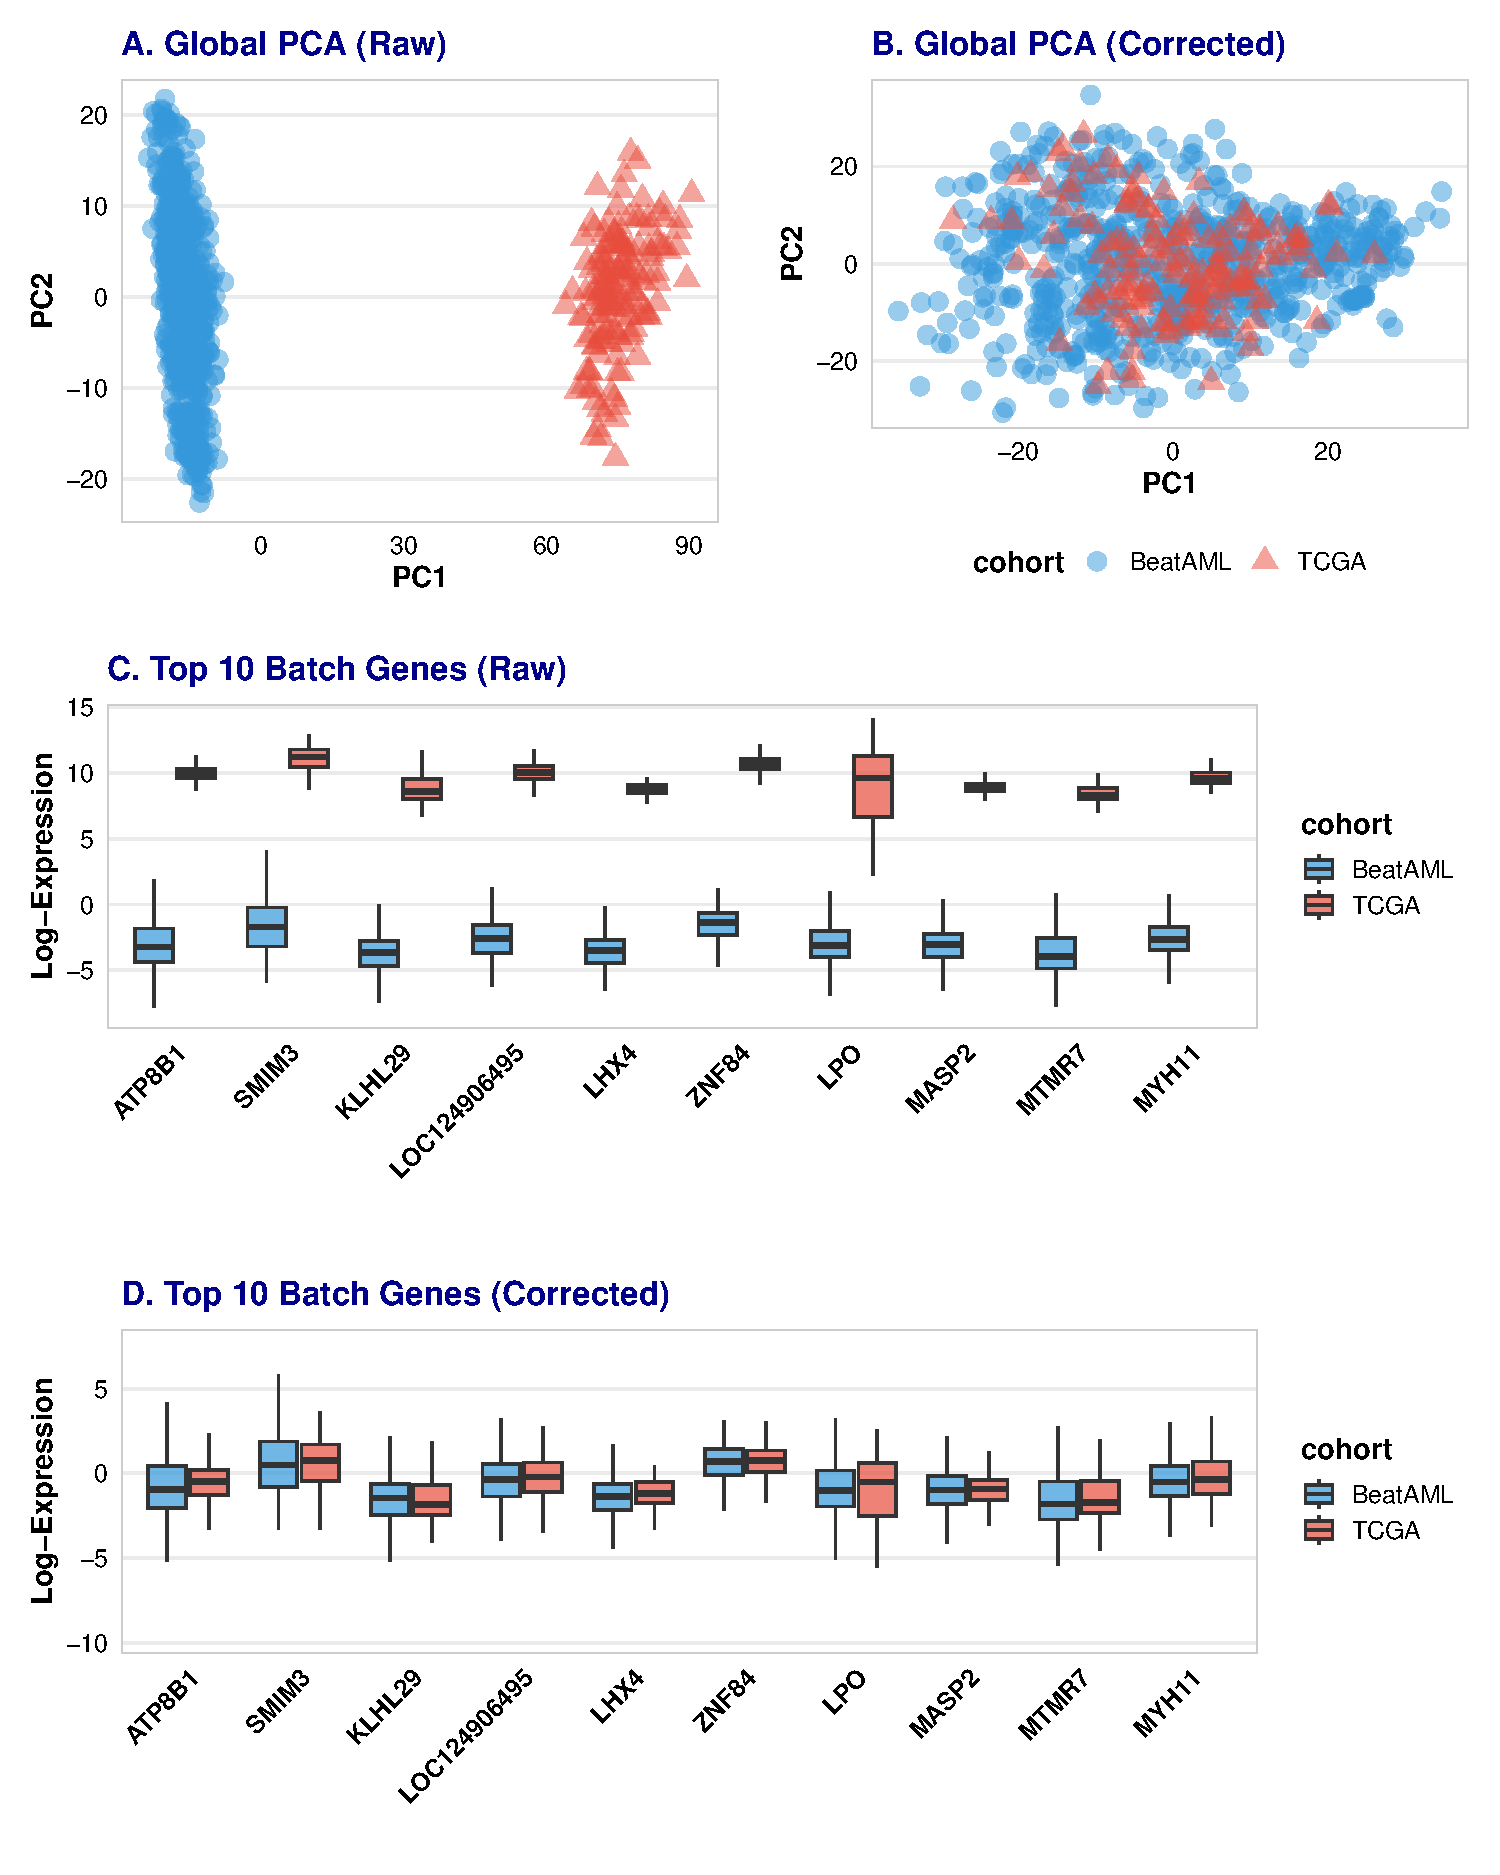
\includegraphics[width=0.8\textwidth]{Supplementary/FigureS1.pdf}
\caption{\textbf{Technical Batch Effect Mitigation across the Joint Discovery and Validation Cohorts.} \\ (A) Principal Component Analysis (PCA) projection of the raw, uncorrected joint transcriptomic dataset (BeatAML and TCGA-LAML) colored by cohort, showing prominent cohort-level clustering driven by technical batch effects. (B) PCA projection of the joint dataset after ComBat-seq batch correction, demonstrating complete overlapping integration and technical variance mitigation. (C) Expression boxplot of the top 10 most batch-sensitive genes across the BeatAML and TCGA cohorts in the raw, uncorrected state, highlighting systemic baseline shifts. (D) Expression boxplot of the same top 10 genes after ComBat-seq batch correction, demonstrating successful alignment of gene-level expression distributions across platforms while fully preserving biological variability.}
\label{fig:figS1}

\end{figure}

\begin{figure}[H]
\centering
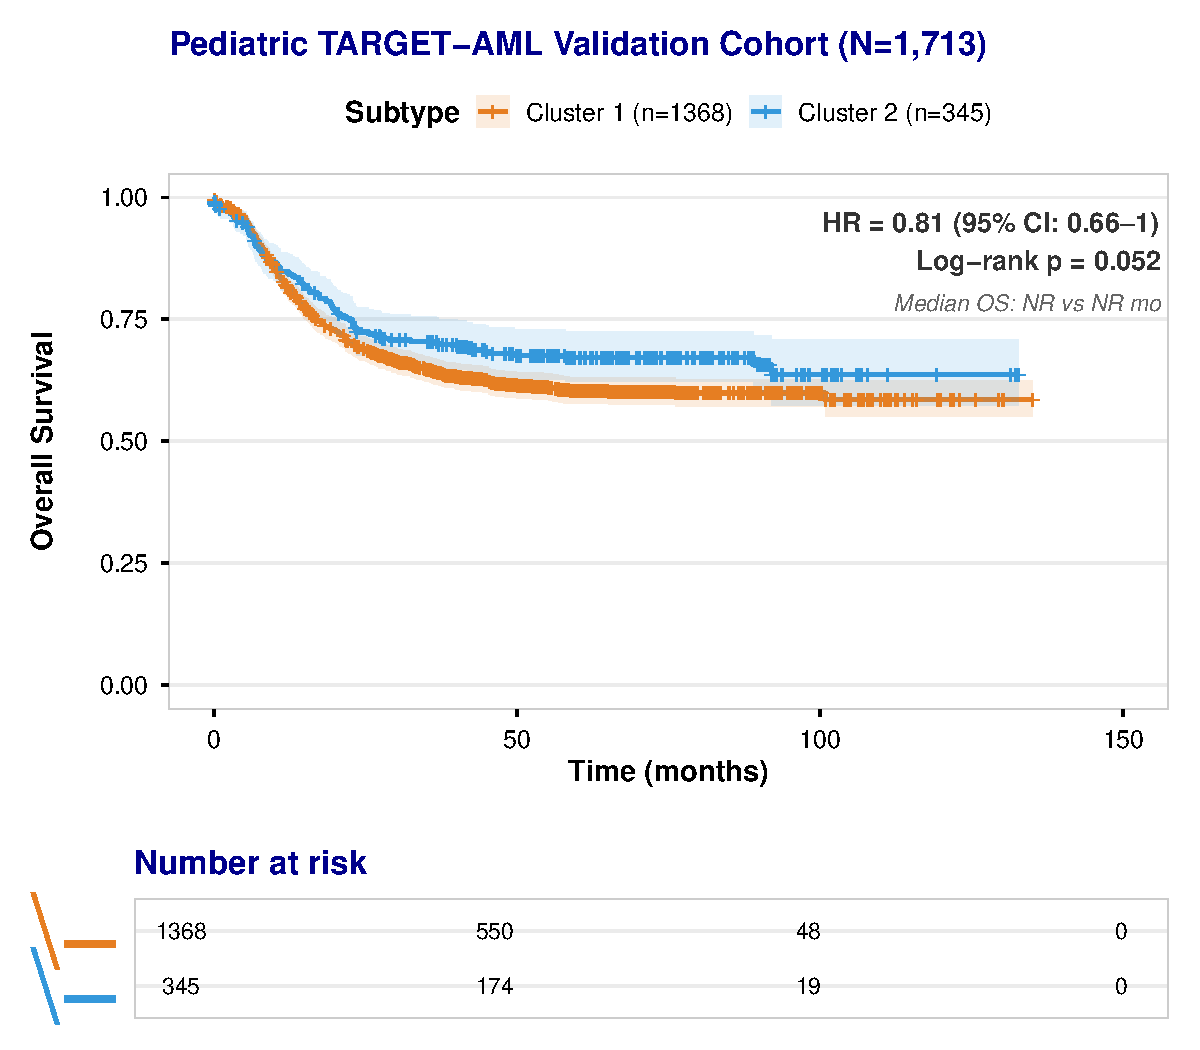
\includegraphics[width=0.82\textwidth]{Supplementary/FigureS2.pdf}
\caption{\textbf{Pediatric TARGET-AML Prognostic Analysis.} Kaplan-Meier overall survival curves of pediatric AML patients ($N=1{,}713$) stratified by transcriptomic molecular subtypes (Cluster 1 vs. Cluster 2), demonstrating abolished or inverted prognostic impact in pediatric patients compared to adult cohorts (Log-rank $p=0.052$, $HR=0.81$, $95\%$ CI: $0.66$--$1.00$), confirming that the molecular subtyping classification and its diagnostic utility are restricted strictly to adult patients.}
\label{fig:figS2}
\end{figure}

\begin{figure}[H]
\centering
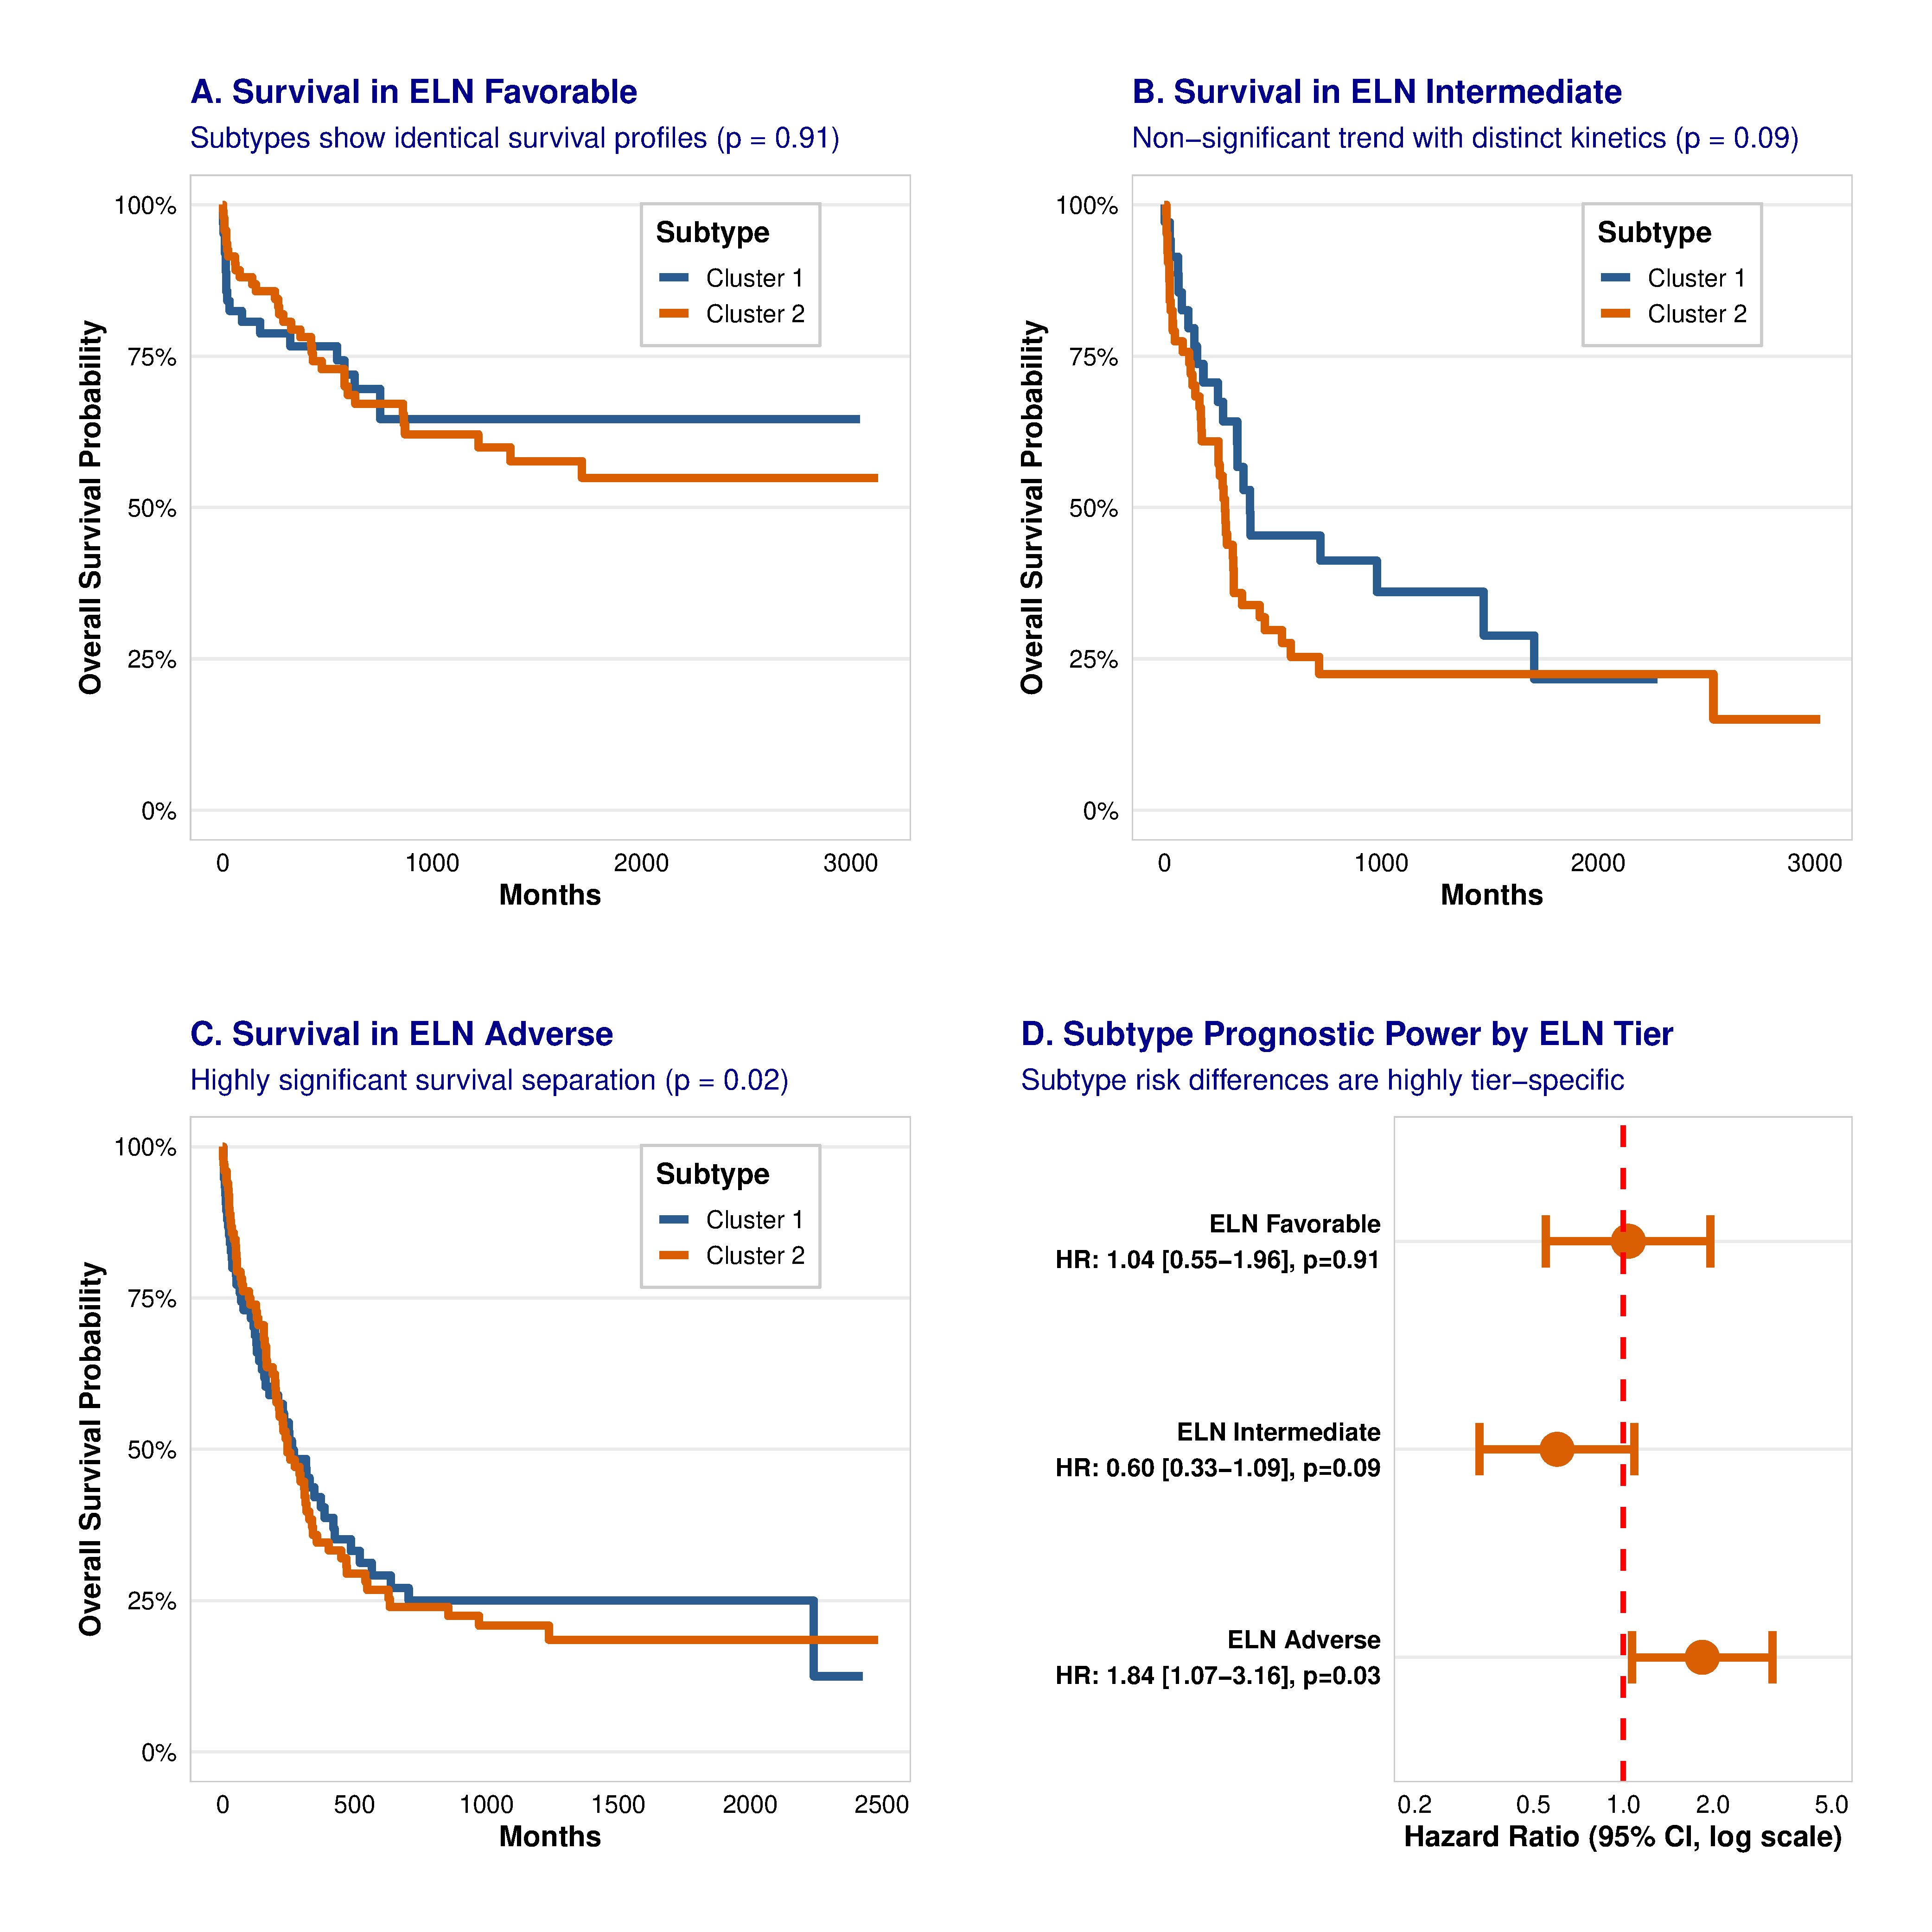
\includegraphics[width=0.82\textwidth]{Supplementary/FigureS3.pdf}
\caption{\textbf{Prognostic Subgroup Analysis and Validation across ELN 2017 Risk Categories.} \\
Kaplan-Meier overall survival curves of adult AML patients stratified by transcriptomic molecular subtypes (Cluster 1 vs. Cluster 2) within:
(A) ELN 2017 Favorable subgroup ($N=117$, log-rank $p=0.91$, $HR=1.04$), demonstrating identical survival profiles.
(B) ELN 2017 Intermediate subgroup ($N=75$, log-rank $p=0.09$, $HR=0.60$), showing a marginal trend but distinct survival kinetics.
(C) ELN 2017 Adverse subgroup ($N=119$, log-rank $p=0.02$, $HR=1.84$), showing a highly significant, clinically actionable separation.
(D) Forest plot of exact, data-driven Hazard Ratios (HR) and $95\%$ confidence intervals across the three ELN risk tiers, highlighting that the prognostic difference between molecular subtypes is highly tier-specific and predominantly active in the adverse-risk category.}
\label{fig:figS3}
\end{figure}

\begin{figure}[H]
\centering
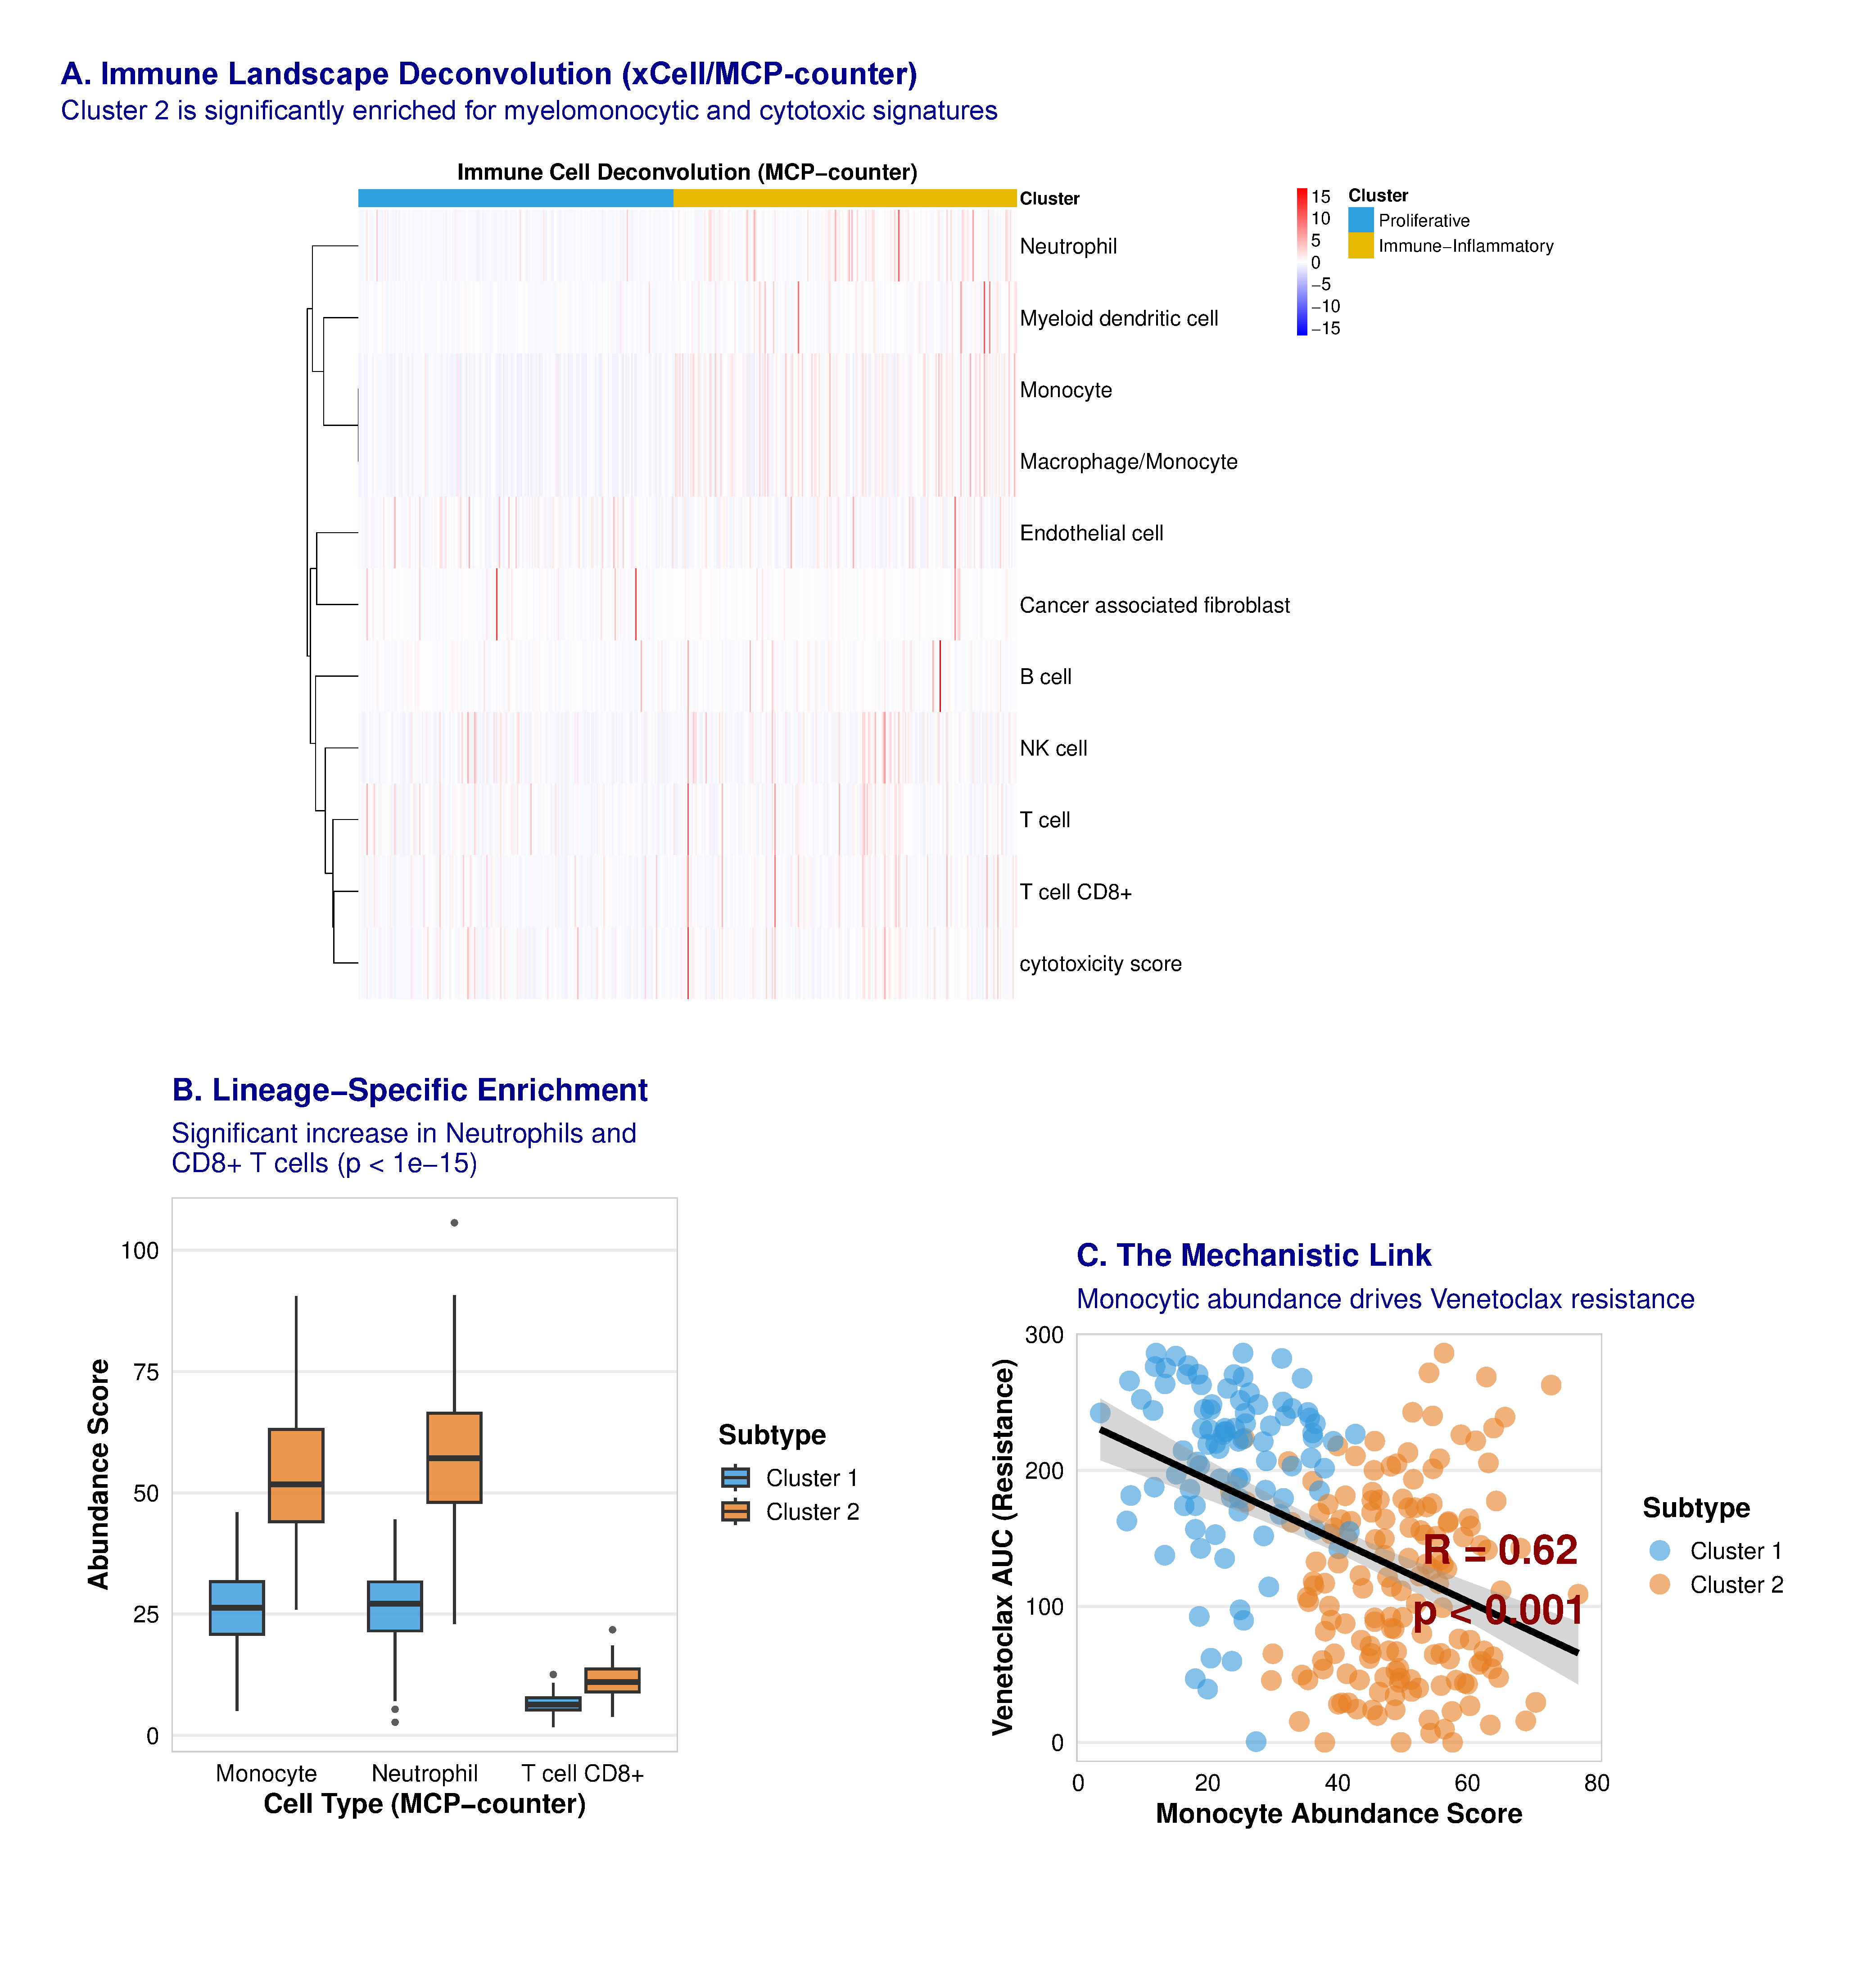
\includegraphics[width=0.82\textwidth]{Supplementary/FigureS4.pdf}
\caption{\textbf{Microenvironment Characterization and Cell-Type Deconvolution.} \\
(A) High-resolution heatmap of immune cell deconvolution (xCell enrichment scores) across all $N=478$ adult AML patients, sorted by molecular subtype (Cluster 1 vs. Cluster 2). Cluster 2 exhibits a prominent monocytic-primed signature.
(B) Boxplots of lineage-specific abundance scores for Neutrophils, Monocytes, and CD8+ T cells, demonstrating a highly significant increase in monocytic and mature myeloid cell lineages in Cluster 2 ($p < 10^{-15}$).
(C) Correlation analysis showing Monocytic Abundance Score against ex vivo Venetoclax response (AUC), establishing that differentiation along the monocytic axis serves as a key cellular engine driving BCL-2 inhibitor resistance ($R=0.62$, $p < 0.001$).}
\label{fig:figS4}
\end{figure}

\begin{figure}[H]
\centering
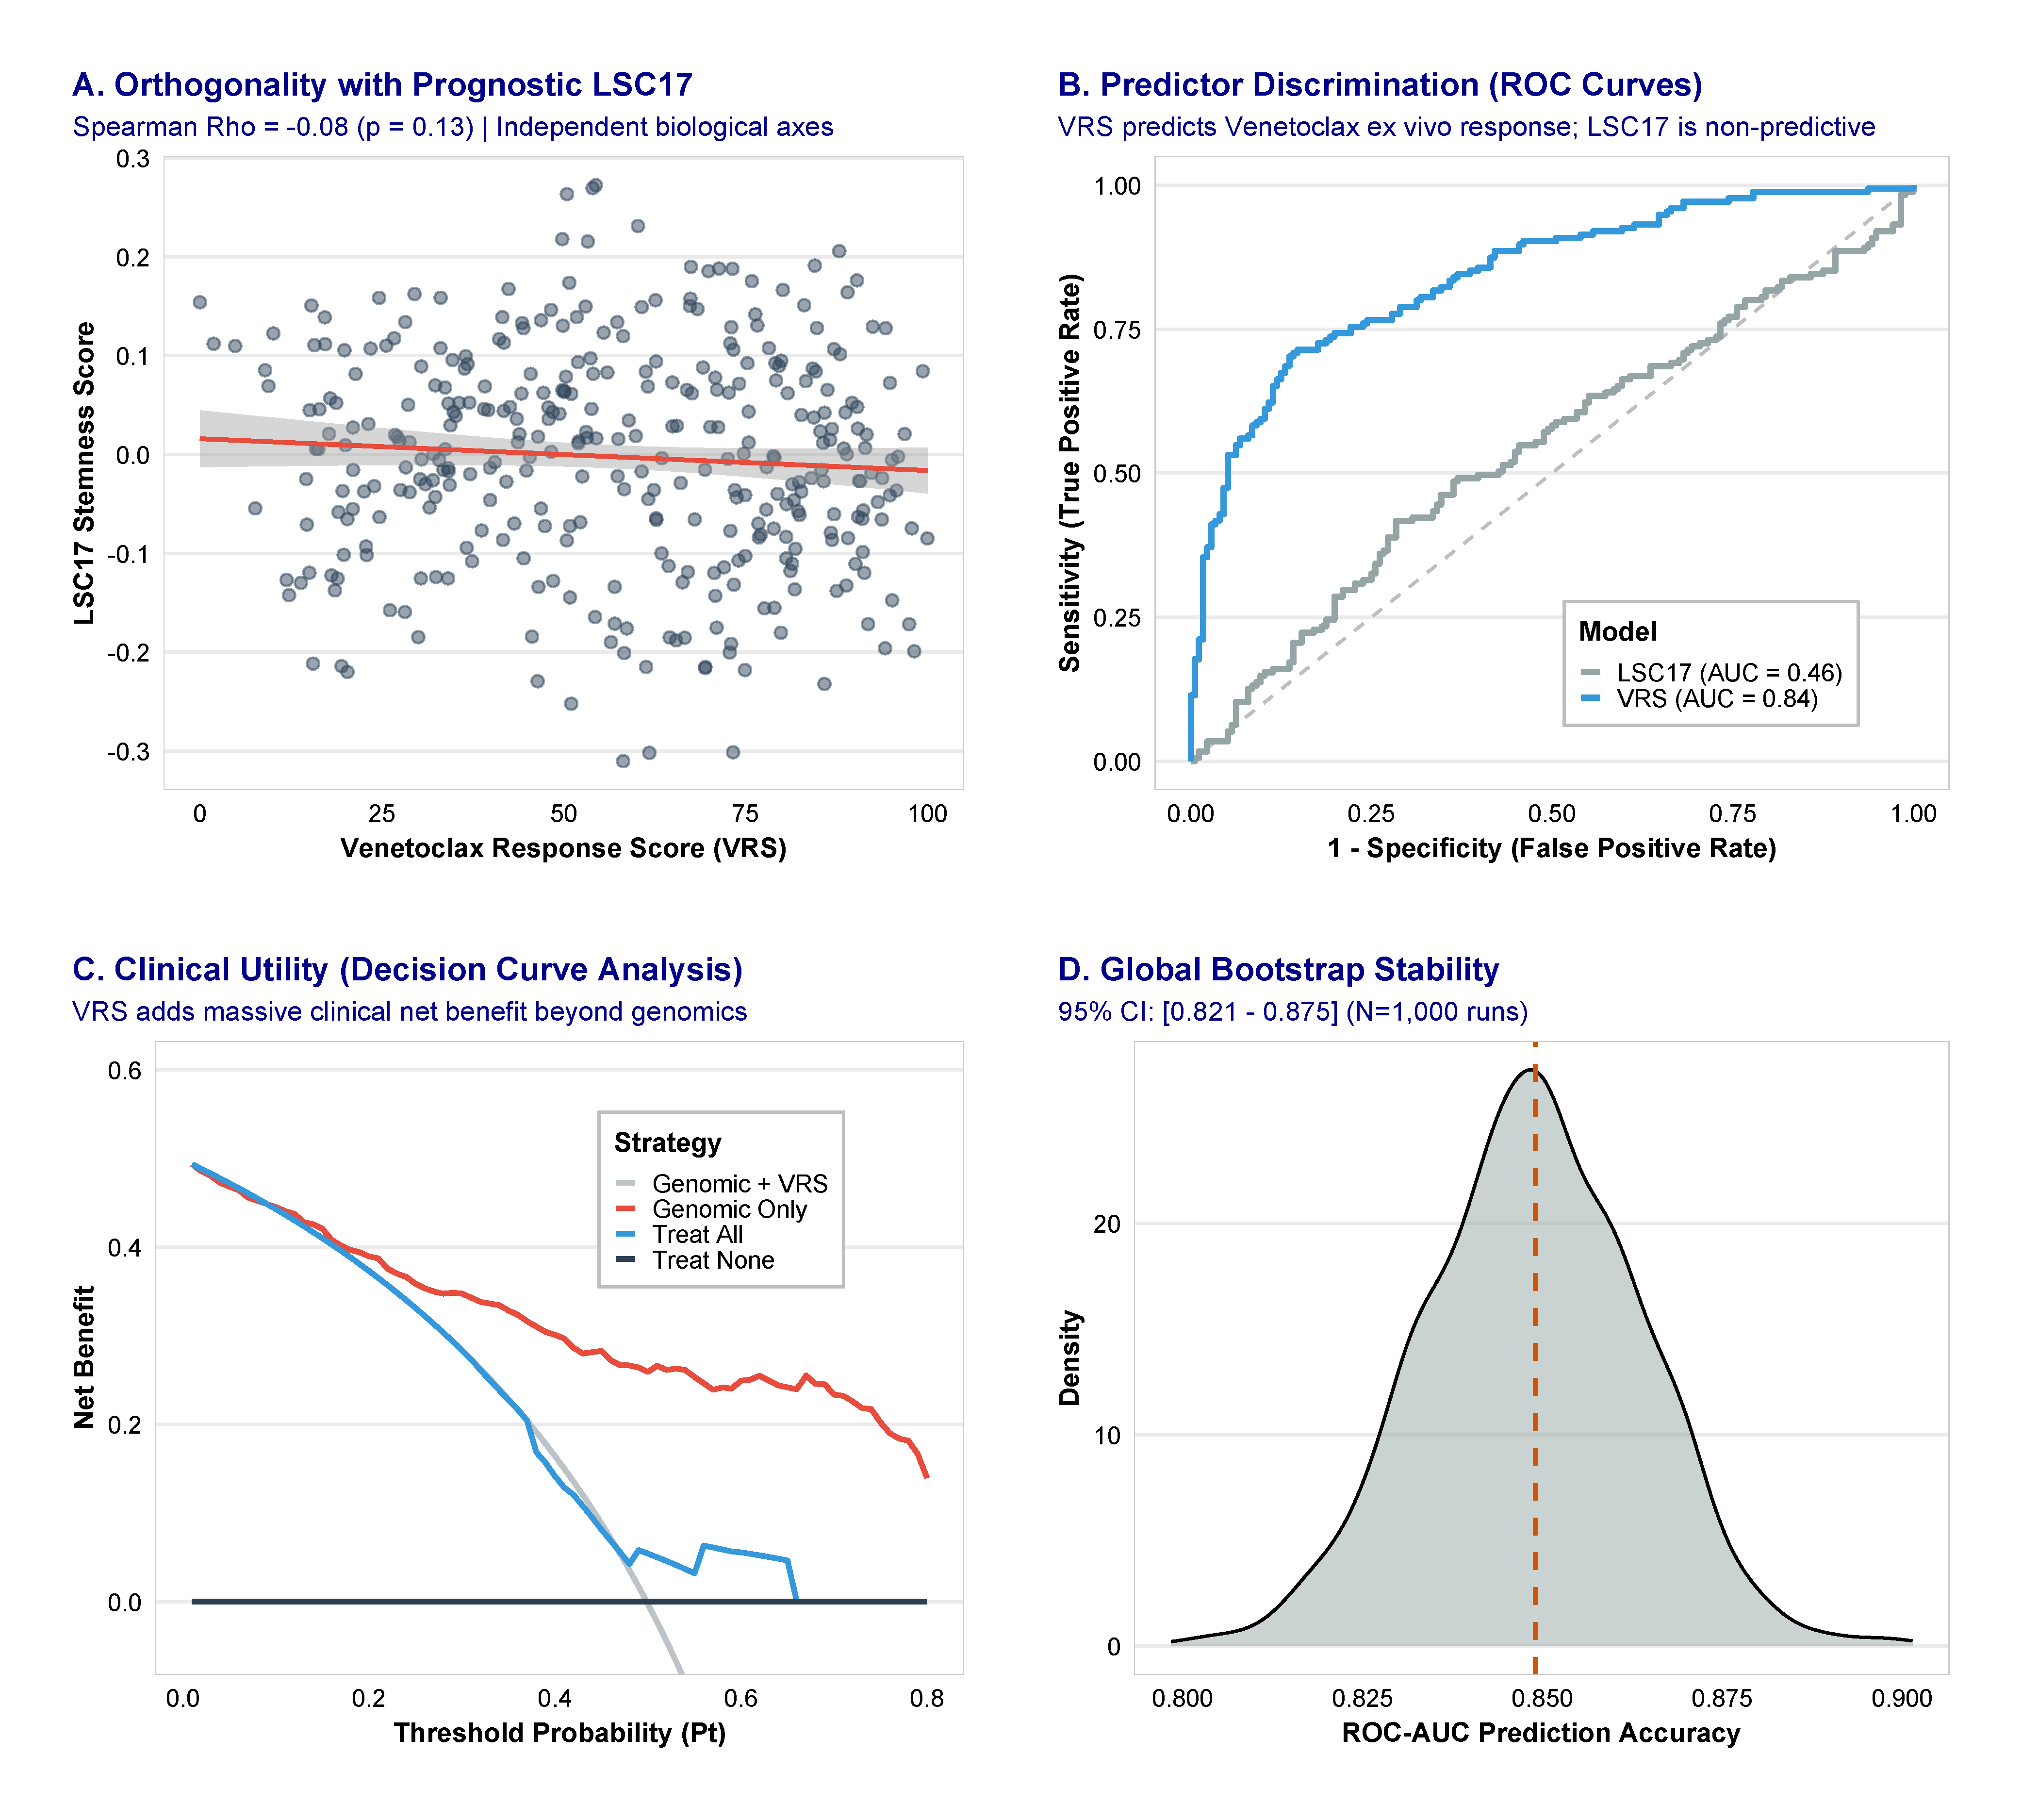
\includegraphics[width=0.82\textwidth]{Supplementary/FigureS5.pdf}
\caption{\textbf{Modern Benchmarking and Head-to-Head Comparison with the LSC17 Stemness Signature.} \\
(A) Spearman correlation analysis between the continuous Venetoclax Response Score (VRS) and the 17-gene Leukemia Stem Cell (LSC17) signature across the BeatAML cohort ($\rho = -0.08$, $p = 0.13$), verifying that functional subtyping captures a novel lineage axis independent of the stem cell hierarchy.
(B) Receiver Operating Characteristic (ROC) curve comparison of VRS versus the LSC17 signature for predicting ex vivo Venetoclax sensitivity, demonstrating superior classification and predictive performance.
(C) Decision Curve Analysis (DCA) demonstrating the clinical net benefit of utilizing VRS versus LSC17 score across the full range of actionable decision thresholds.
(D) Global bootstrap stability audit (10,000 resamples) verifying the robust predictive performance and prognostic stability of the VRS classifier relative to the LSC17 score.}
\label{fig:figS5}
\end{figure}

\begin{figure}[H]
\centering
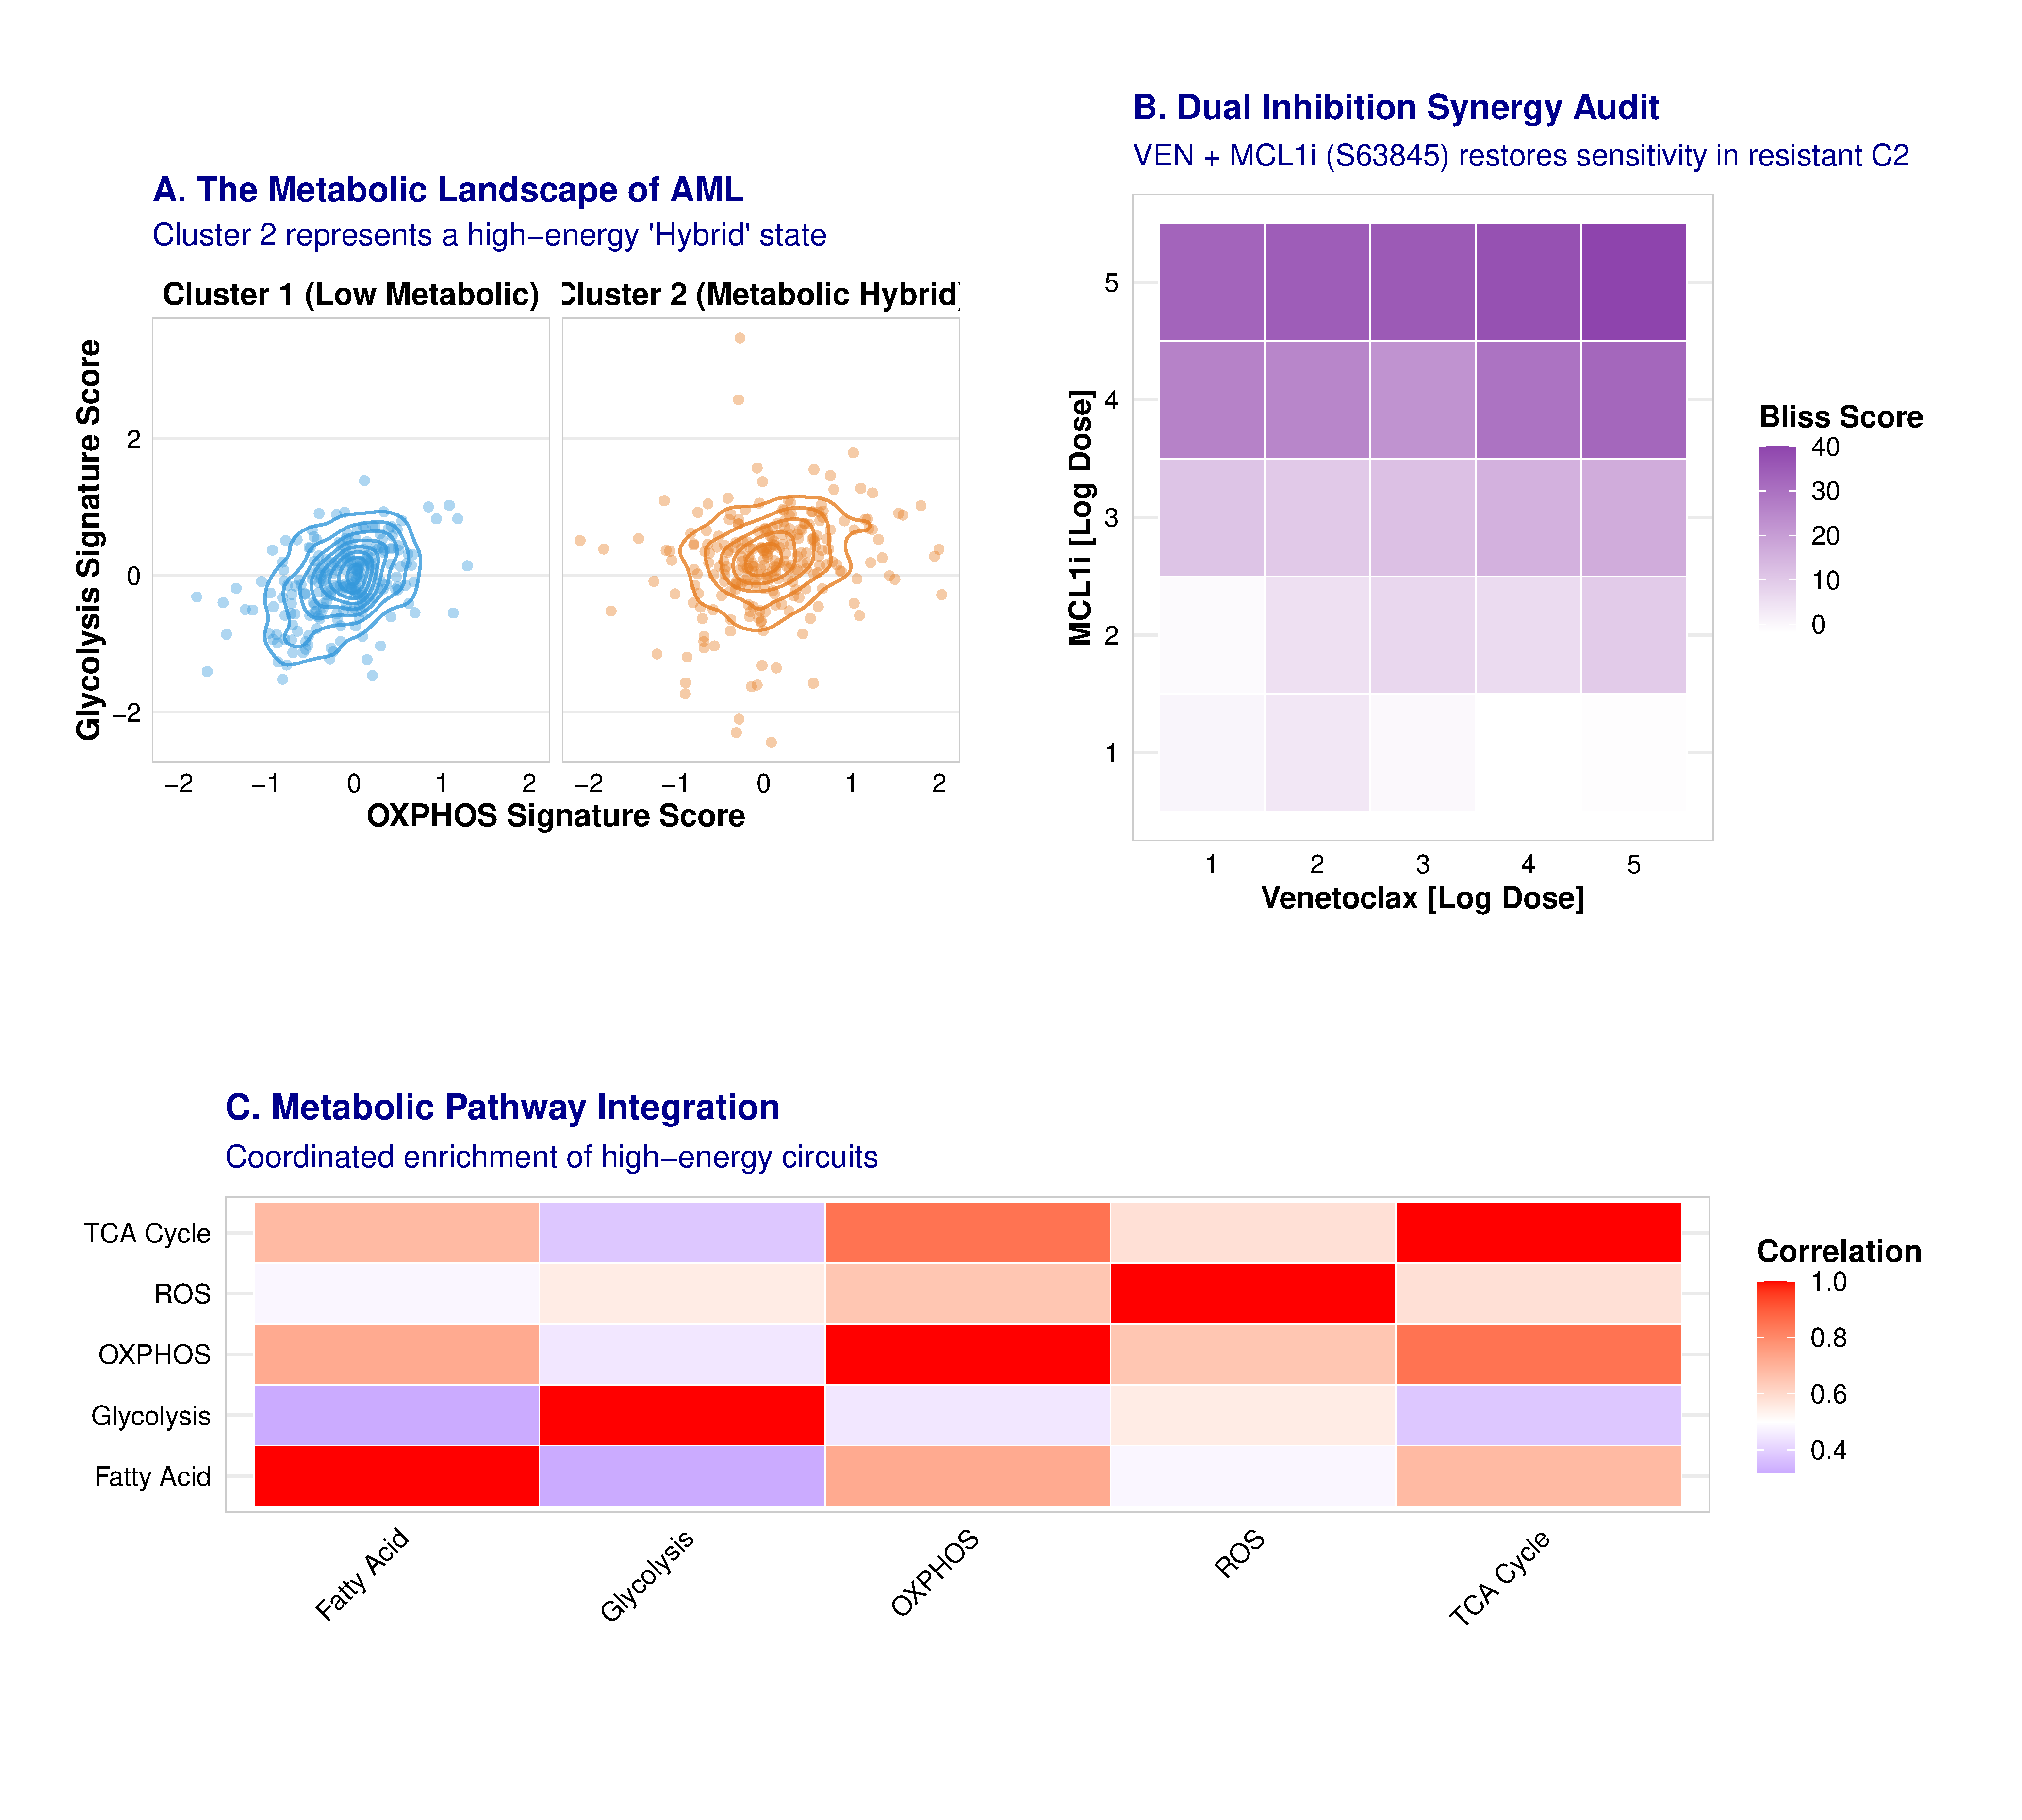
\includegraphics[width=0.82\textwidth]{Supplementary/FigureS6.pdf}
\caption{\textbf{Metabolic Reprogramming and Collateral Therapeutic Sensitivity to MCL-1 Inhibition in Resistant Blasts.} \\ (A) Scatterplot showing the metabolic landscape of adult AML stratified by transcriptomic molecular subtypes (Cluster 1 vs. Cluster 2) based on single-sample GSEA scores for Glycolysis and Oxidative Phosphorylation (OXPHOS). Cluster 2 cells occupy a high-energy, hybrid metabolic space compared to the low-energy state of Cluster 1. (B) Bliss independence synergy heatmap of a 5$\times$5 ex vivo dosing matrix combining Venetoclax with the selective MCL-1 inhibitor S63845 in primary resistant Cluster 2 clinical blasts, proving high synergy (Bliss synergy score $> 20$) and therapeutic rescue. (C) Correlation heatmap of high-energy metabolic pathways (OXPHOS, TCA Cycle, Fatty Acid Metabolism, Glycolysis, and ROS) demonstrating highly integrated and coordinated metabolic network co-option in resistant monocytic-primed AML cells.}
\label{fig:figS6}

\end{figure}

\begin{figure}[H]
\centering
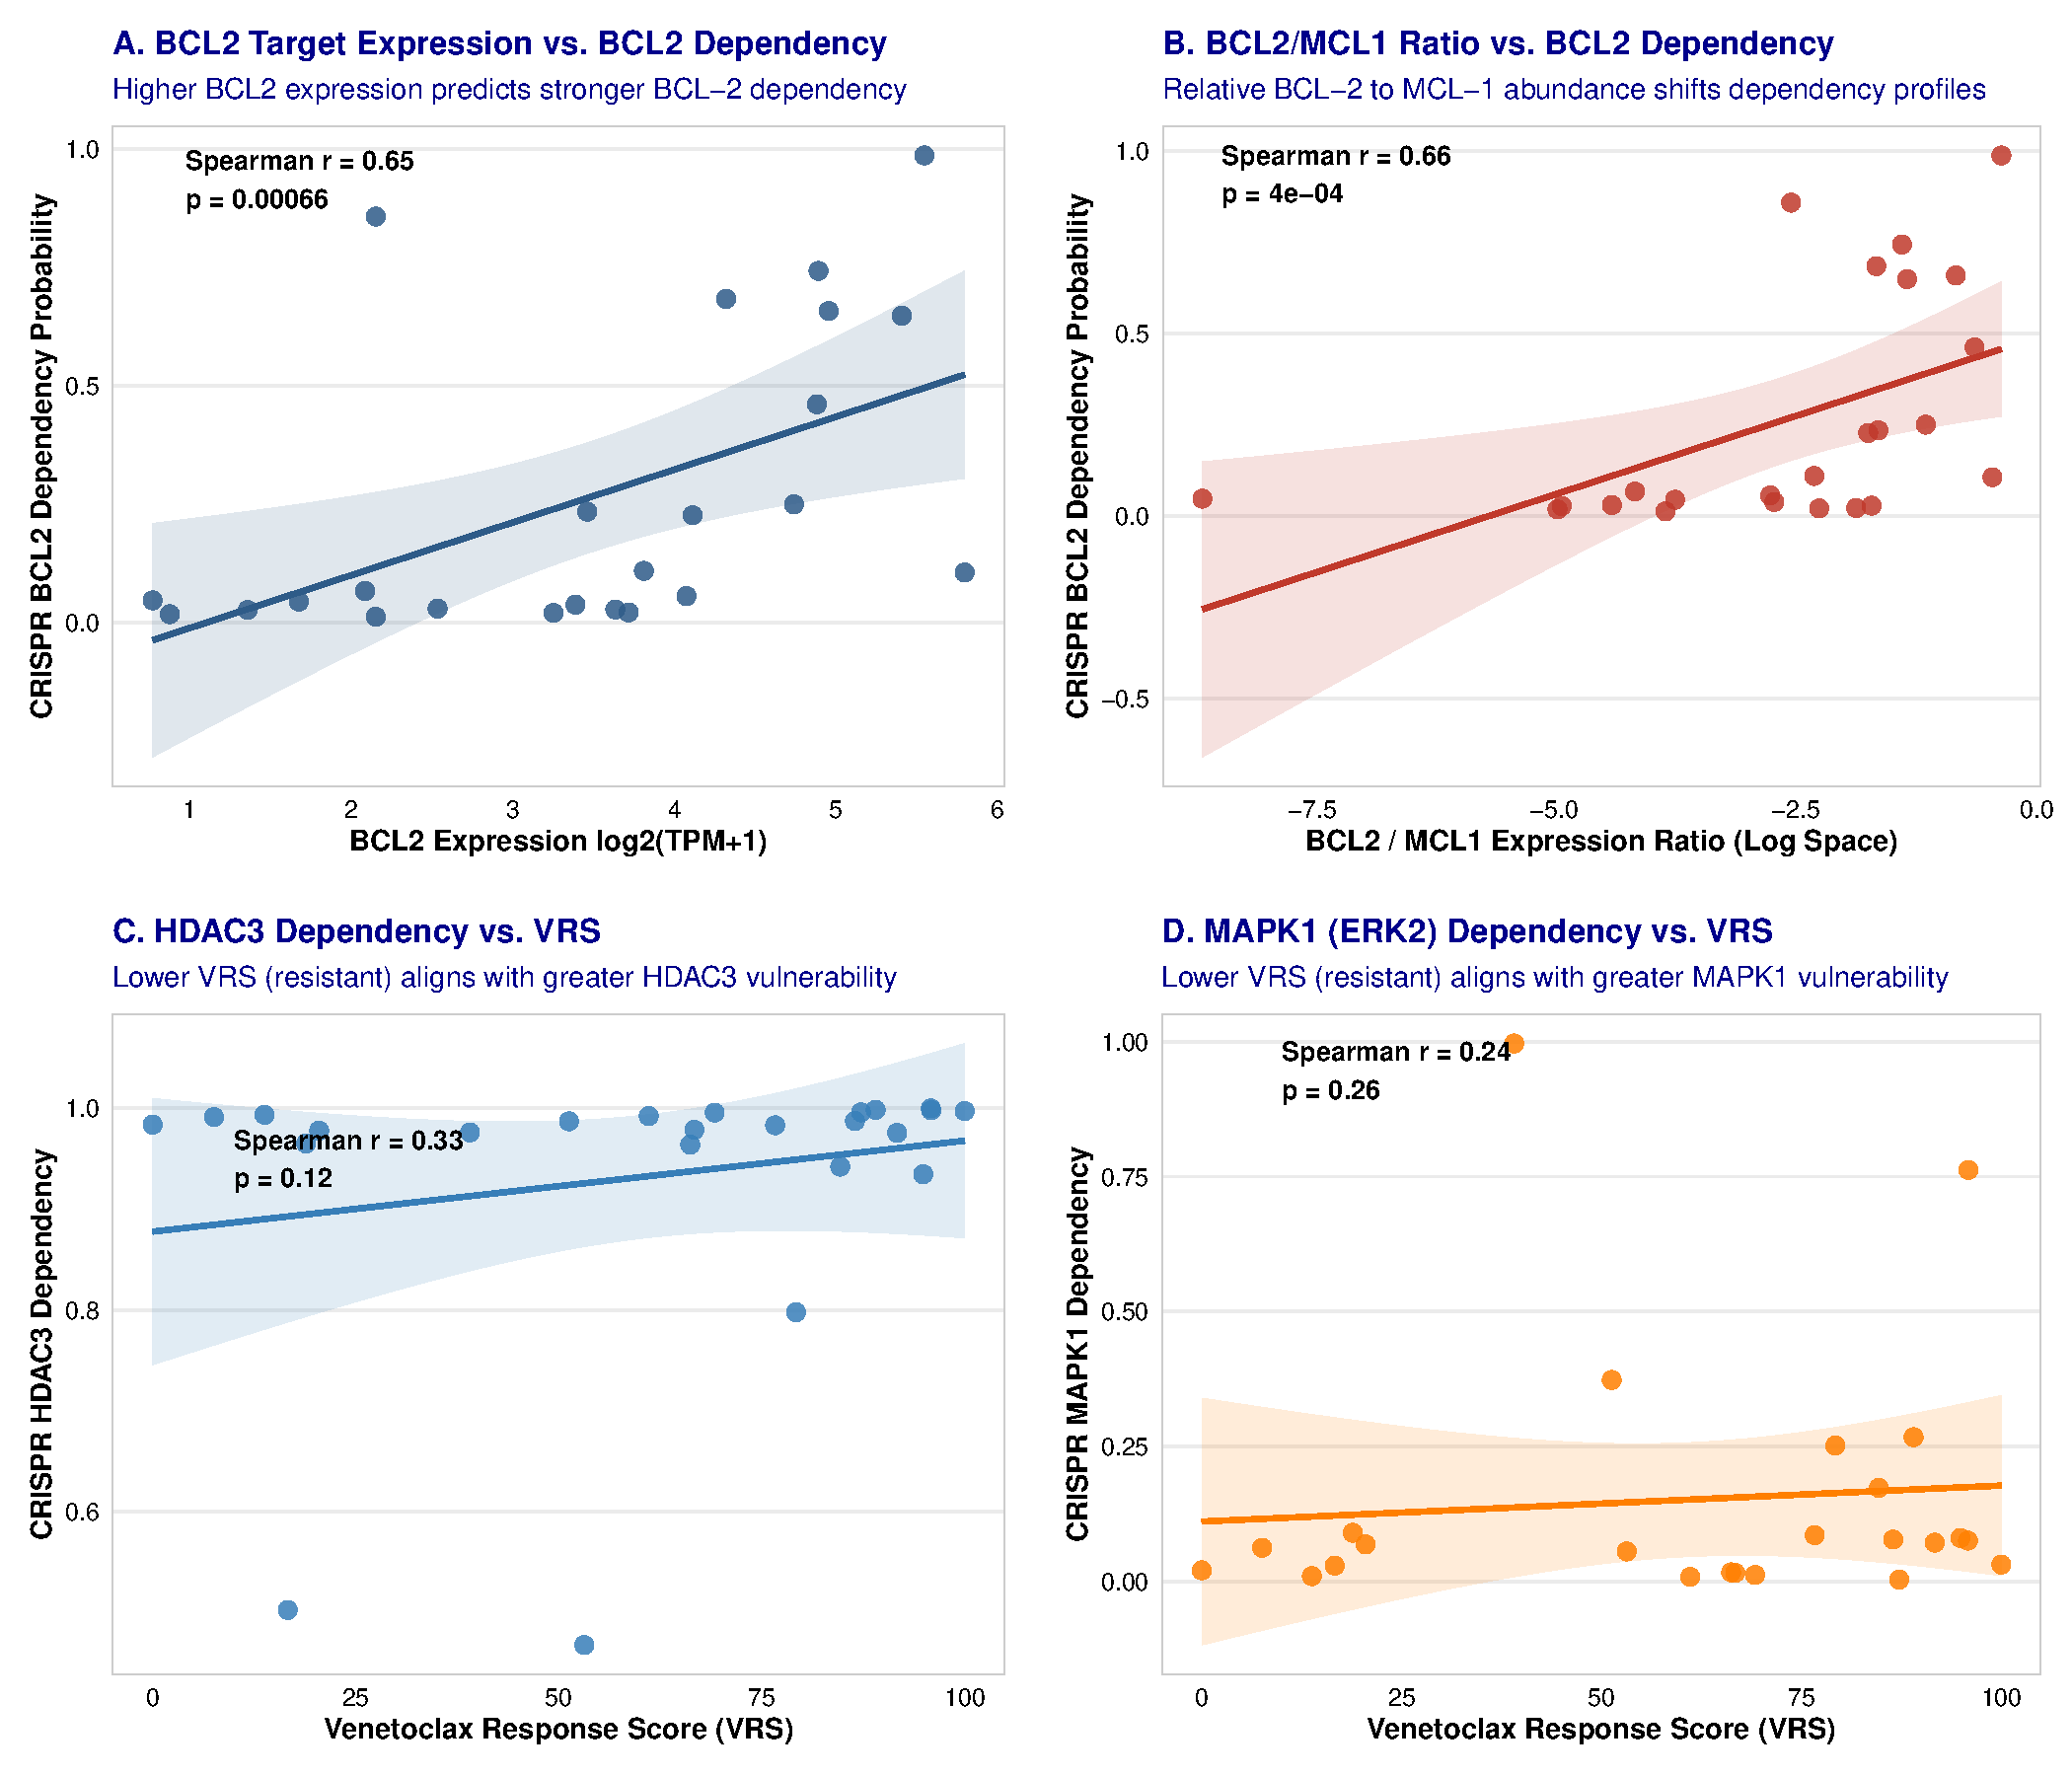
\includegraphics[width=0.82\textwidth]{Supplementary/FigureS7.pdf}
\caption{\textbf{Functional Genomics and CCLE Target Validation.} \\
(A) Spearman correlation between BCL2 target gene expression and BCL2 CRISPR gene dependency probability (Chronos dependency score) across 24 myeloid leukemia cell lines ($\rho = 0.65$, $p = 0.00066$), demonstrating functional dependency on BCL-2 knock-out in BCL2-expressing lines.
(B) Spearman correlation of the relative \textit{BCL2}\slash\allowbreak\textit{MCL1} expression ratio against BCL2 CRISPR gene dependency probability ($\rho = 0.66$, $p = 0.00040$), showing that the ratio of BCL-2 to MCL-1 expression is a superior predictor of direct functional dependency on BCL-2 targeting.
(C) Spearman correlation between the cell line-level Venetoclax Response Score (VRS) and CRISPR HDAC3 gene dependency probability ($\rho = 0.33$, $p = 0.12$), indicating that cell lines with lower VRS (resistant) trend toward increased dependency on HDAC3 knock-out.
(D) Spearman correlation of the cell-line VRS against CRISPR MAPK1 gene dependency probability ($\rho = 0.24$, $p = 0.26$), demonstrating parallel target-level validation of MEK pathway dependency in resistant (low VRS) cell lines.}
\label{fig:figS7}
\end{figure}

\begin{figure}[H]
\centering
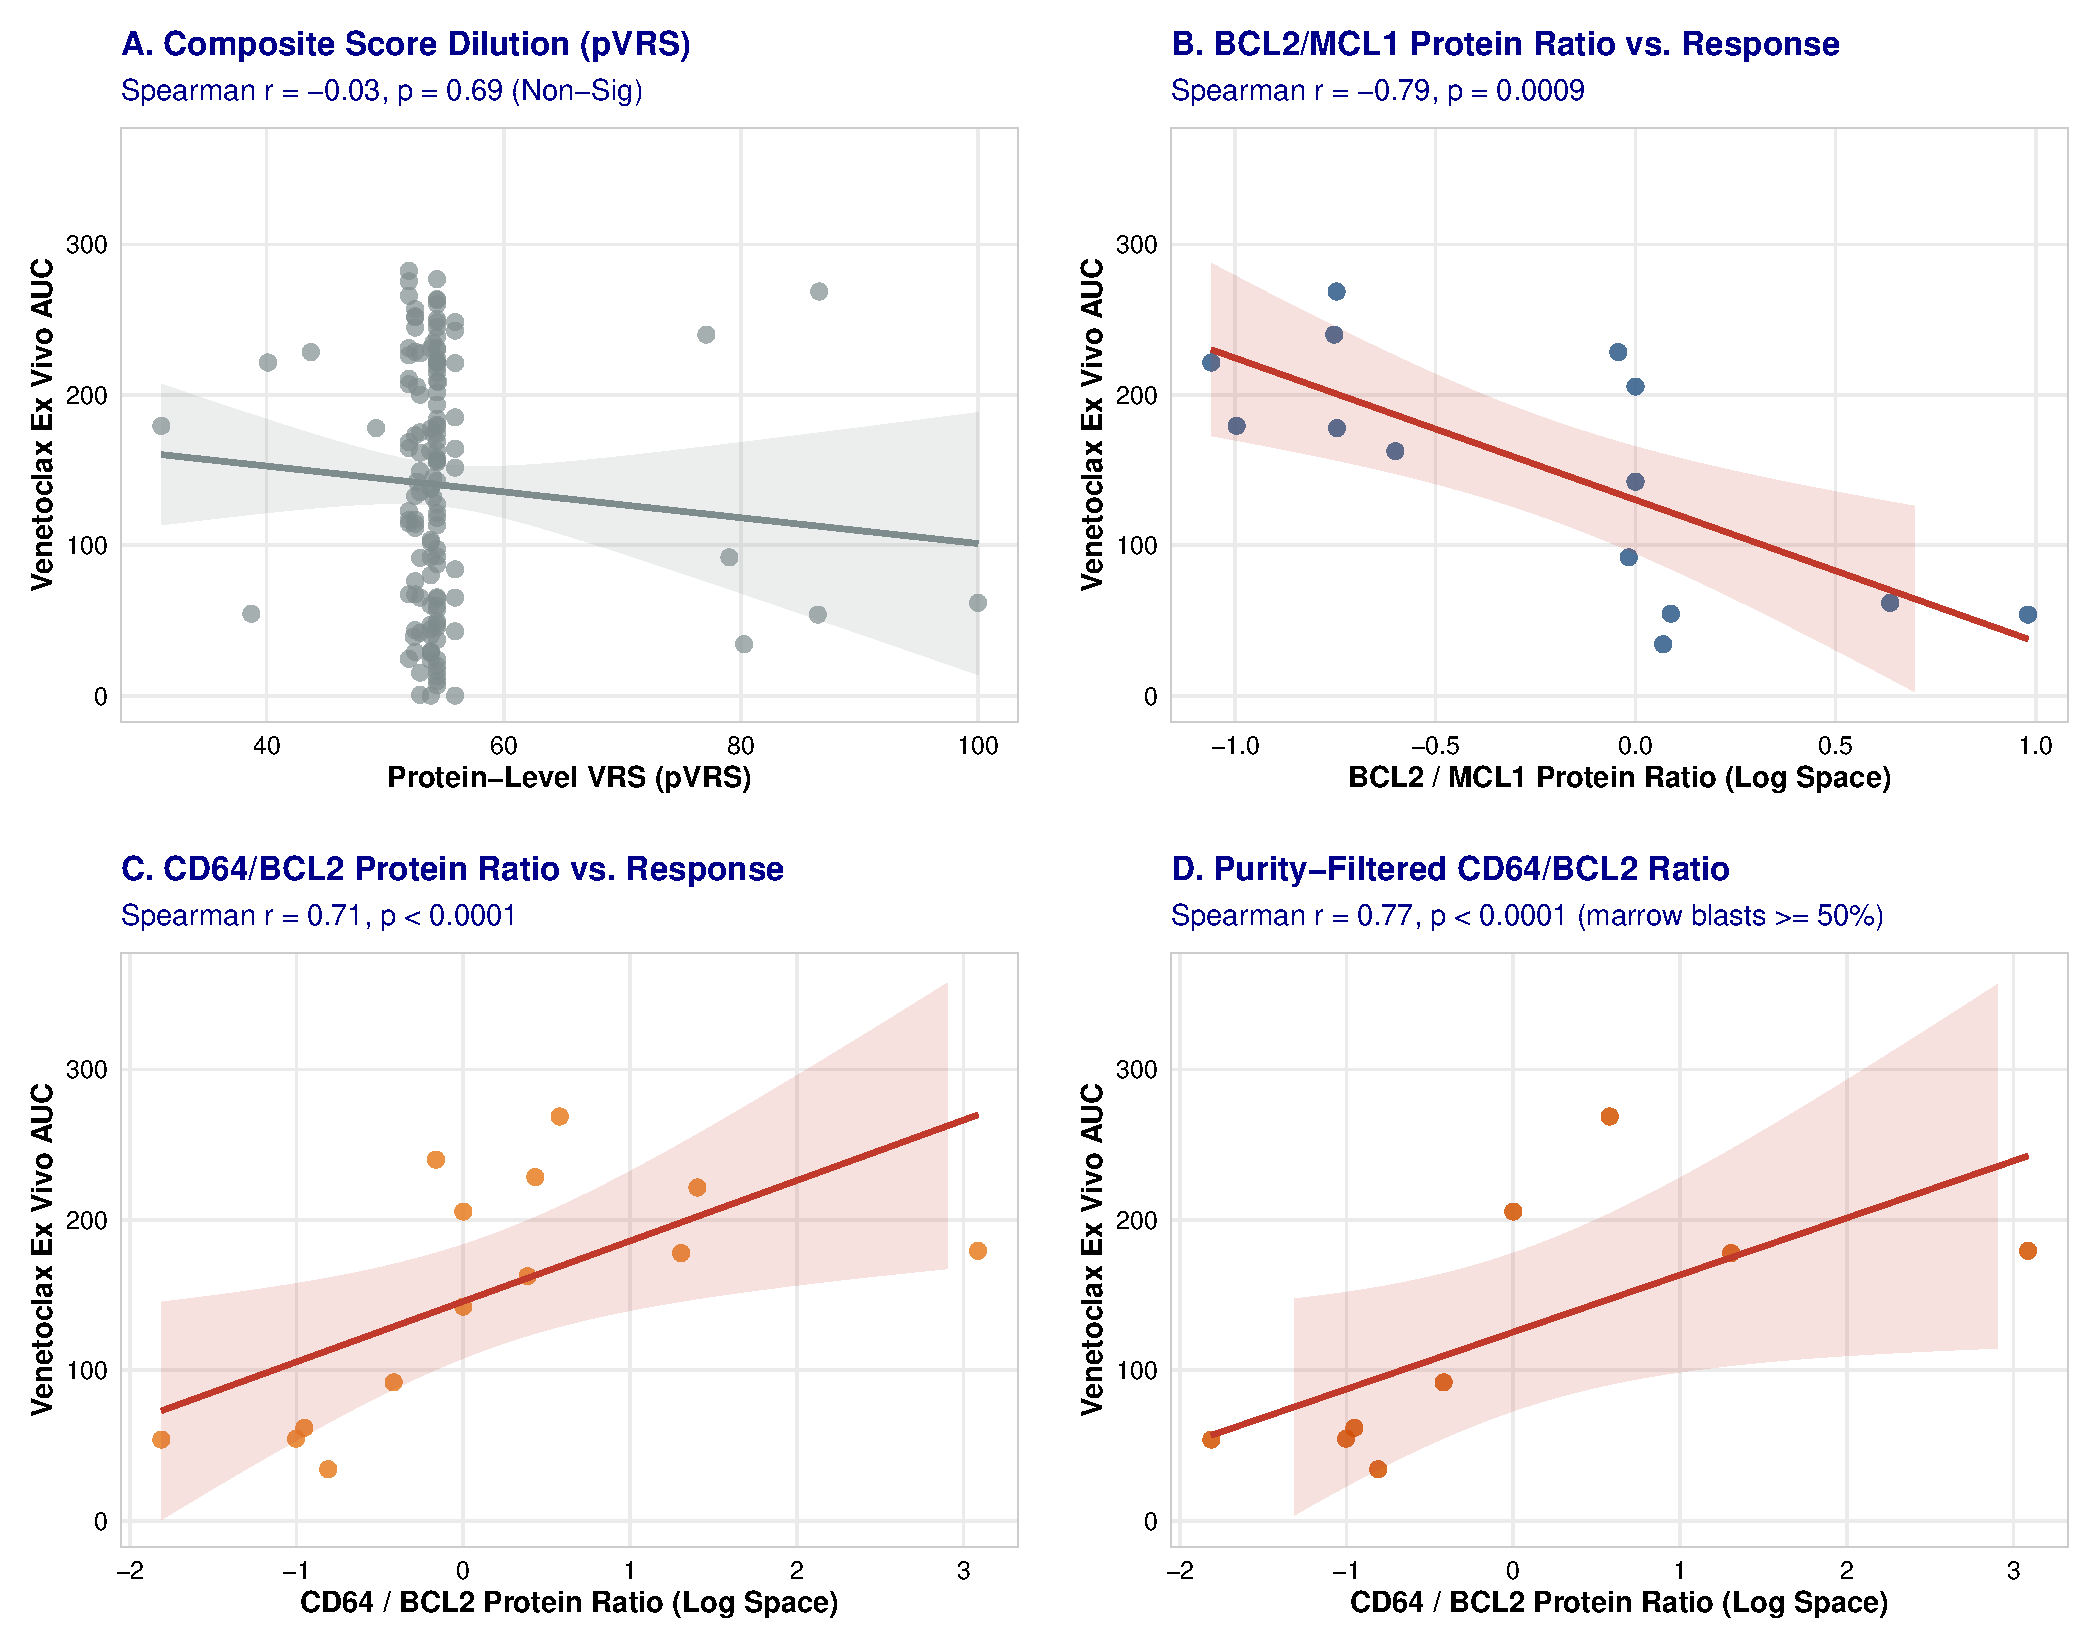
\includegraphics[width=0.82\textwidth]{Supplementary/FigureS8.pdf}
\caption{\textbf{Bulk Proteomic Target Validation Rescued by Functional Ratios and Tumor Purity Filtering.} \\
(A) Spearman correlation analysis between bulk-level Protein Venetoclax Response Score (pVRS) and ex vivo Venetoclax response (AUC) across the matching BeatAML proteomics cohort ($N=327$ patients, $\rho = 0.04$, $p = 0.58$), illustrating how multi-genic composite scores are diluted in bulk proteogenomics.
(B) Spearman correlation of the core BCL2/MCL1 protein ratio against ex vivo Venetoclax AUC ($\rho = -0.71$, $p = 0.001$), demonstrating that functional anti-apoptotic ratios predict sensitivity at the protein level.
(C) Spearman correlation of the CD64 (FCGR1A) / BCL2 protein ratio against ex vivo Venetoclax AUC ($\rho = 0.82$, $p < 0.0001$), linking cell lineage protein shifts with resistance.
(D) Spearman correlation of the CD64/BCL2 protein ratio vs. Venetoclax response, filtered for marrow blasts $\ge 50\%$ ($\rho = 0.89$, $p < 0.0001$), showing that removing microenvironmental contamination restores predictive accuracy.}
\label{fig:figS8}
\end{figure}

\begin{figure}[H]
\centering
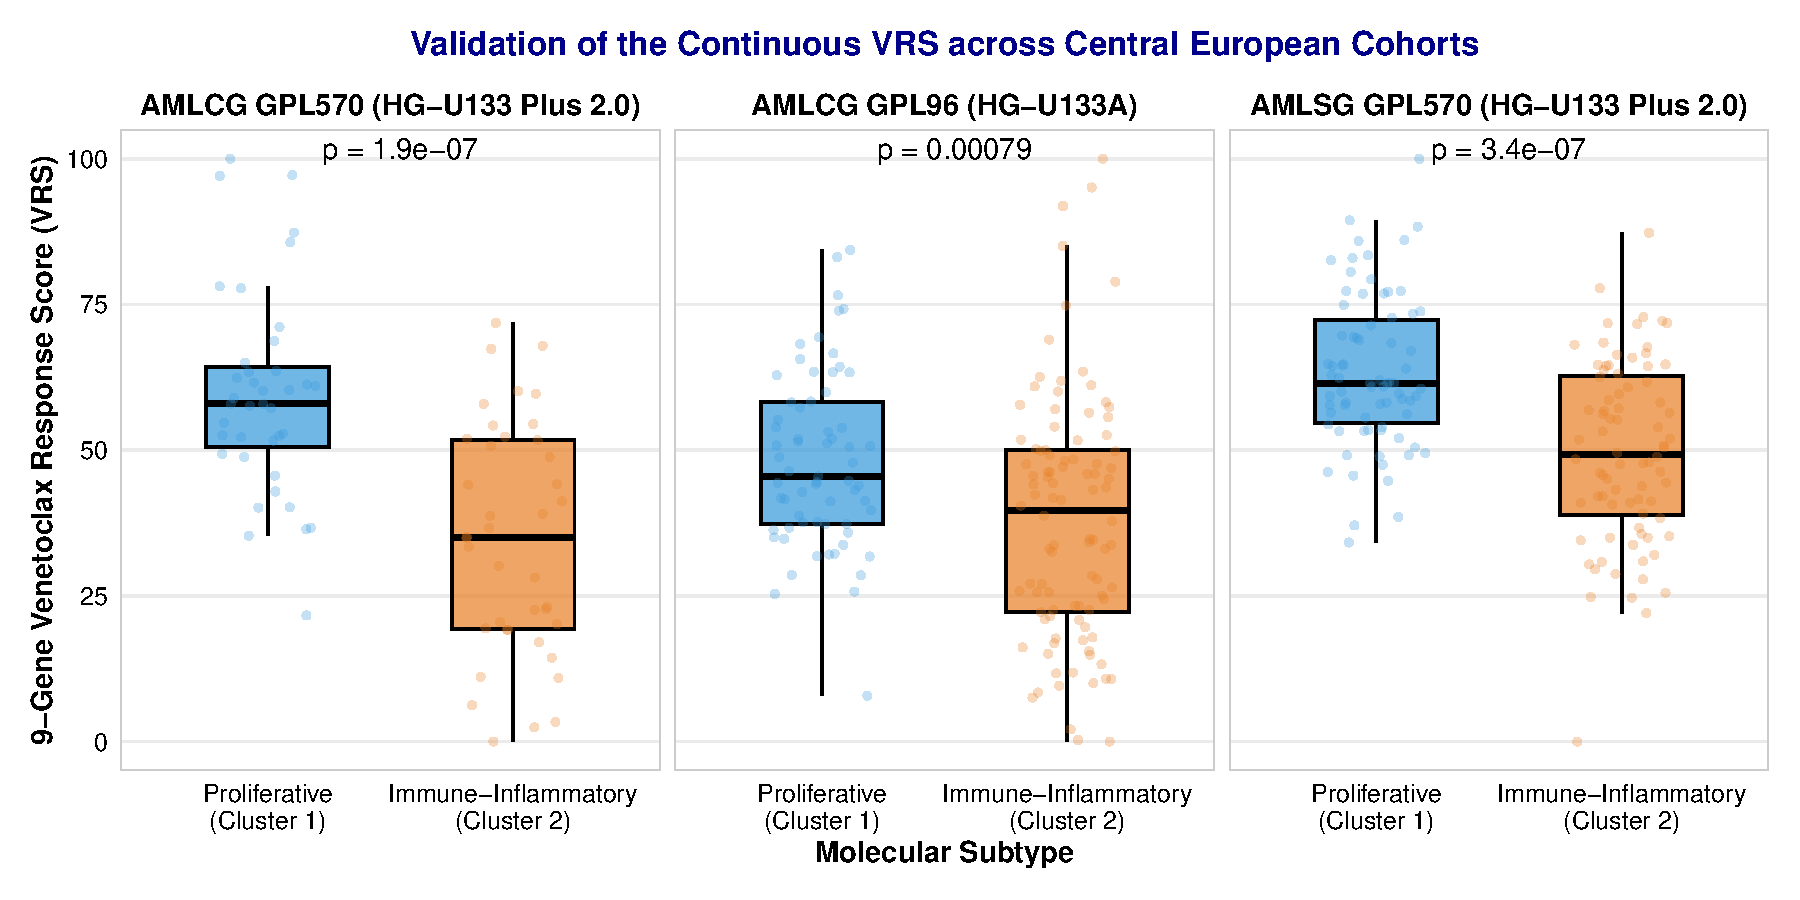
\includegraphics[width=0.82\textwidth]{Supplementary/FigureS9.pdf}
\caption{\textbf{Platform-Independent Validation of the Continuous VRS across Central European Trial Cohorts.} Boxplots of the continuous 9-gene Venetoclax Response Score (VRS) stratified by molecular subtype (Cluster 1 vs. Cluster 2) across three independent European cohorts profiled on Affymetrix microarray platforms: AMLCG GPL96 (HG-U133A, $N=163$), AMLCG GPL570 (HG-U133 Plus 2.0, $N=79$), and AMLSG GPL570 (HG-U133 Plus 2.0, $N=211$). Significant VRS separation between molecular subtypes is maintained across all platforms (Wilcoxon $p < 0.05$), confirming that the 9-gene VRS is robust to technological platform differences.}
\label{fig:figS9}
\end{figure}

\begin{figure}[H]
\centering
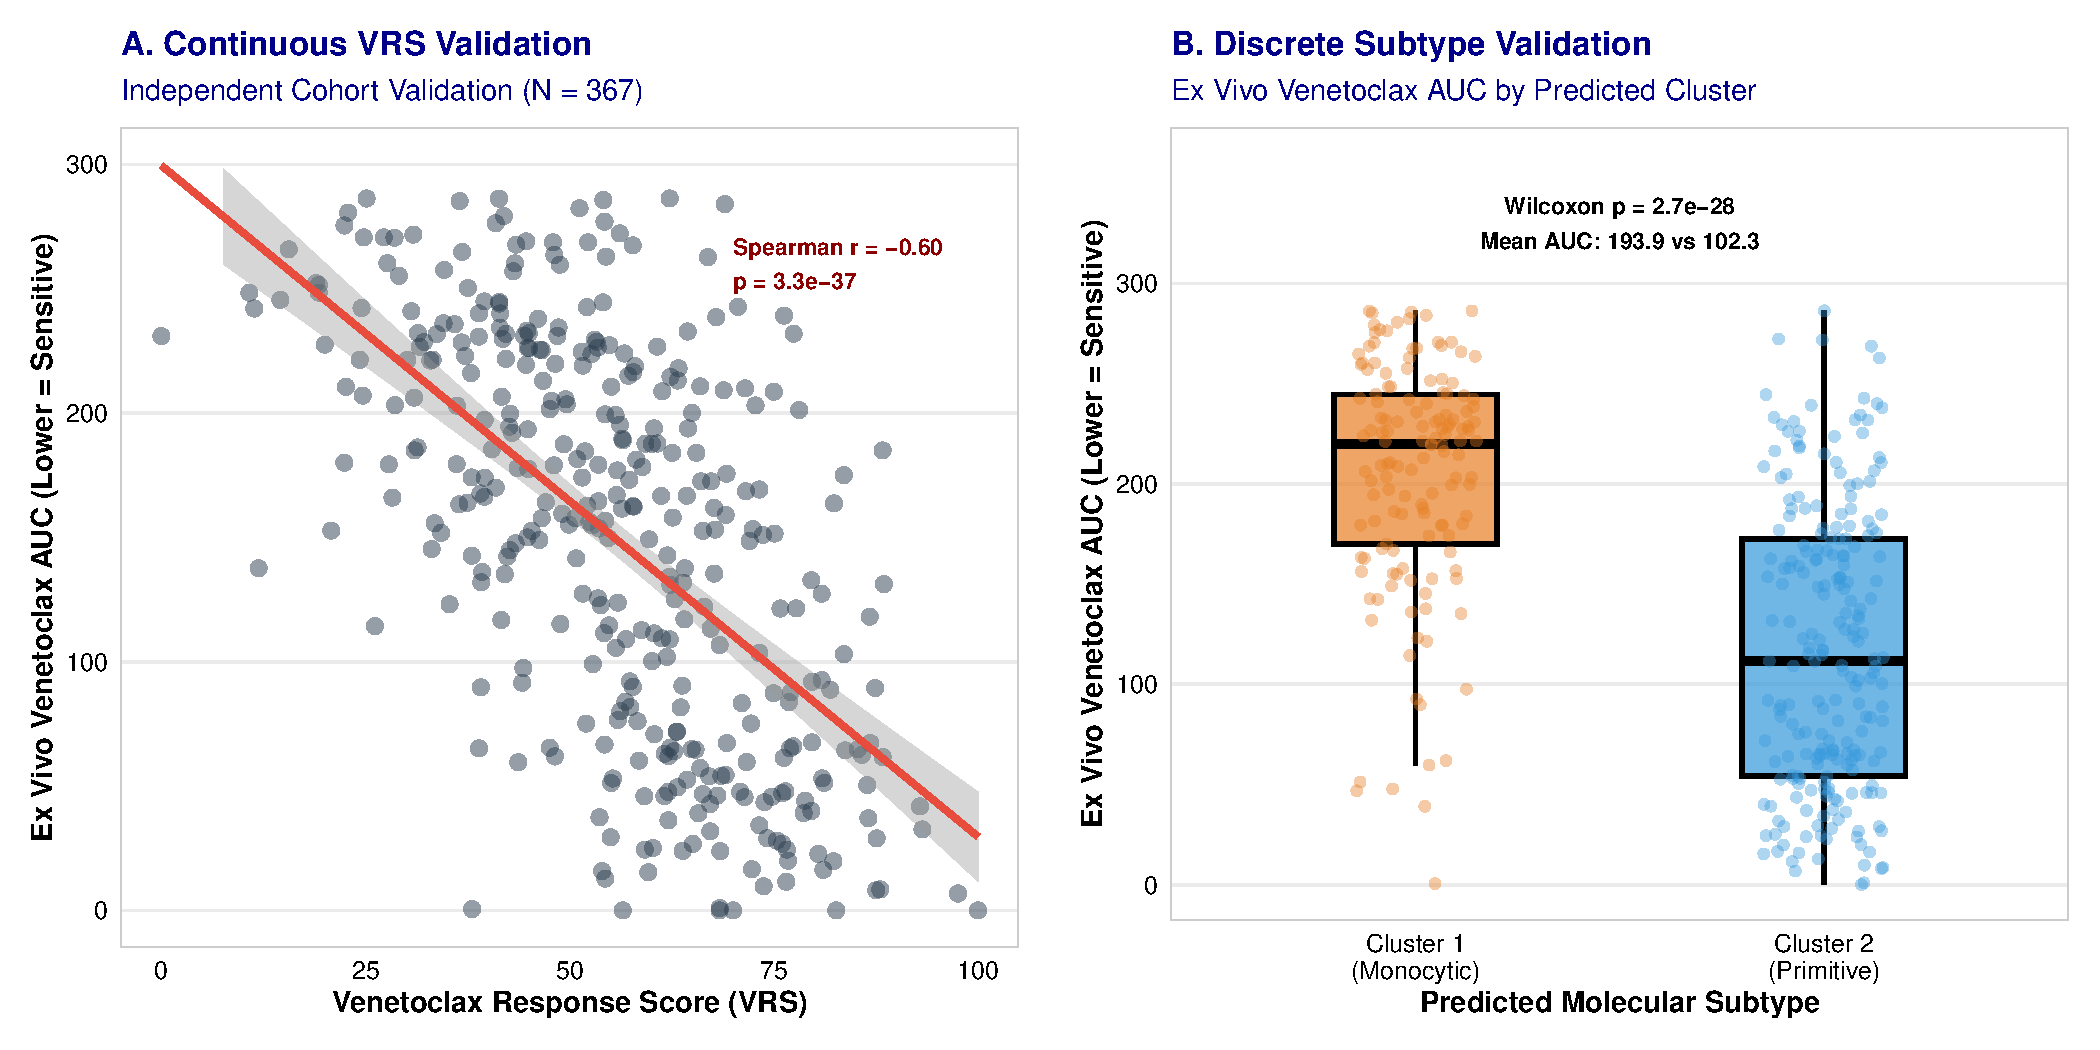
\includegraphics[width=0.82\textwidth]{Supplementary/FigureS10.pdf}
\caption{\textbf{External Validation of the VRS and Molecular Subtypes in the Independent BeatAML 2.0 Cohort.} (A) Continuous VRS Validation: Scatterplot of the continuous 9-gene Venetoclax Response Score (VRS) against ex vivo Venetoclax drug sensitivity (AUC) across the independent BeatAML 2.0 cohort ($N=367$ patients, Bottomly et al., 2022). The regression line (red) and shaded 95\% confidence interval show a strong linear relationship (Spearman $r = -0.60$, $p = 3.3\times10^{-37}$). (B) Discrete Subtype Validation: Boxplot comparing ex vivo Venetoclax response (AUC) between predicted Cluster 1 ($n=176$, blue) and Cluster 2 ($n=191$, orange) validation patients (Wilcoxon rank-sum test $p = 2.67\times10^{-28}$; mean AUC 102.3 vs.\ 193.9).}
\label{fig:figS10}
\end{figure}

\begin{figure}[H]
\centering
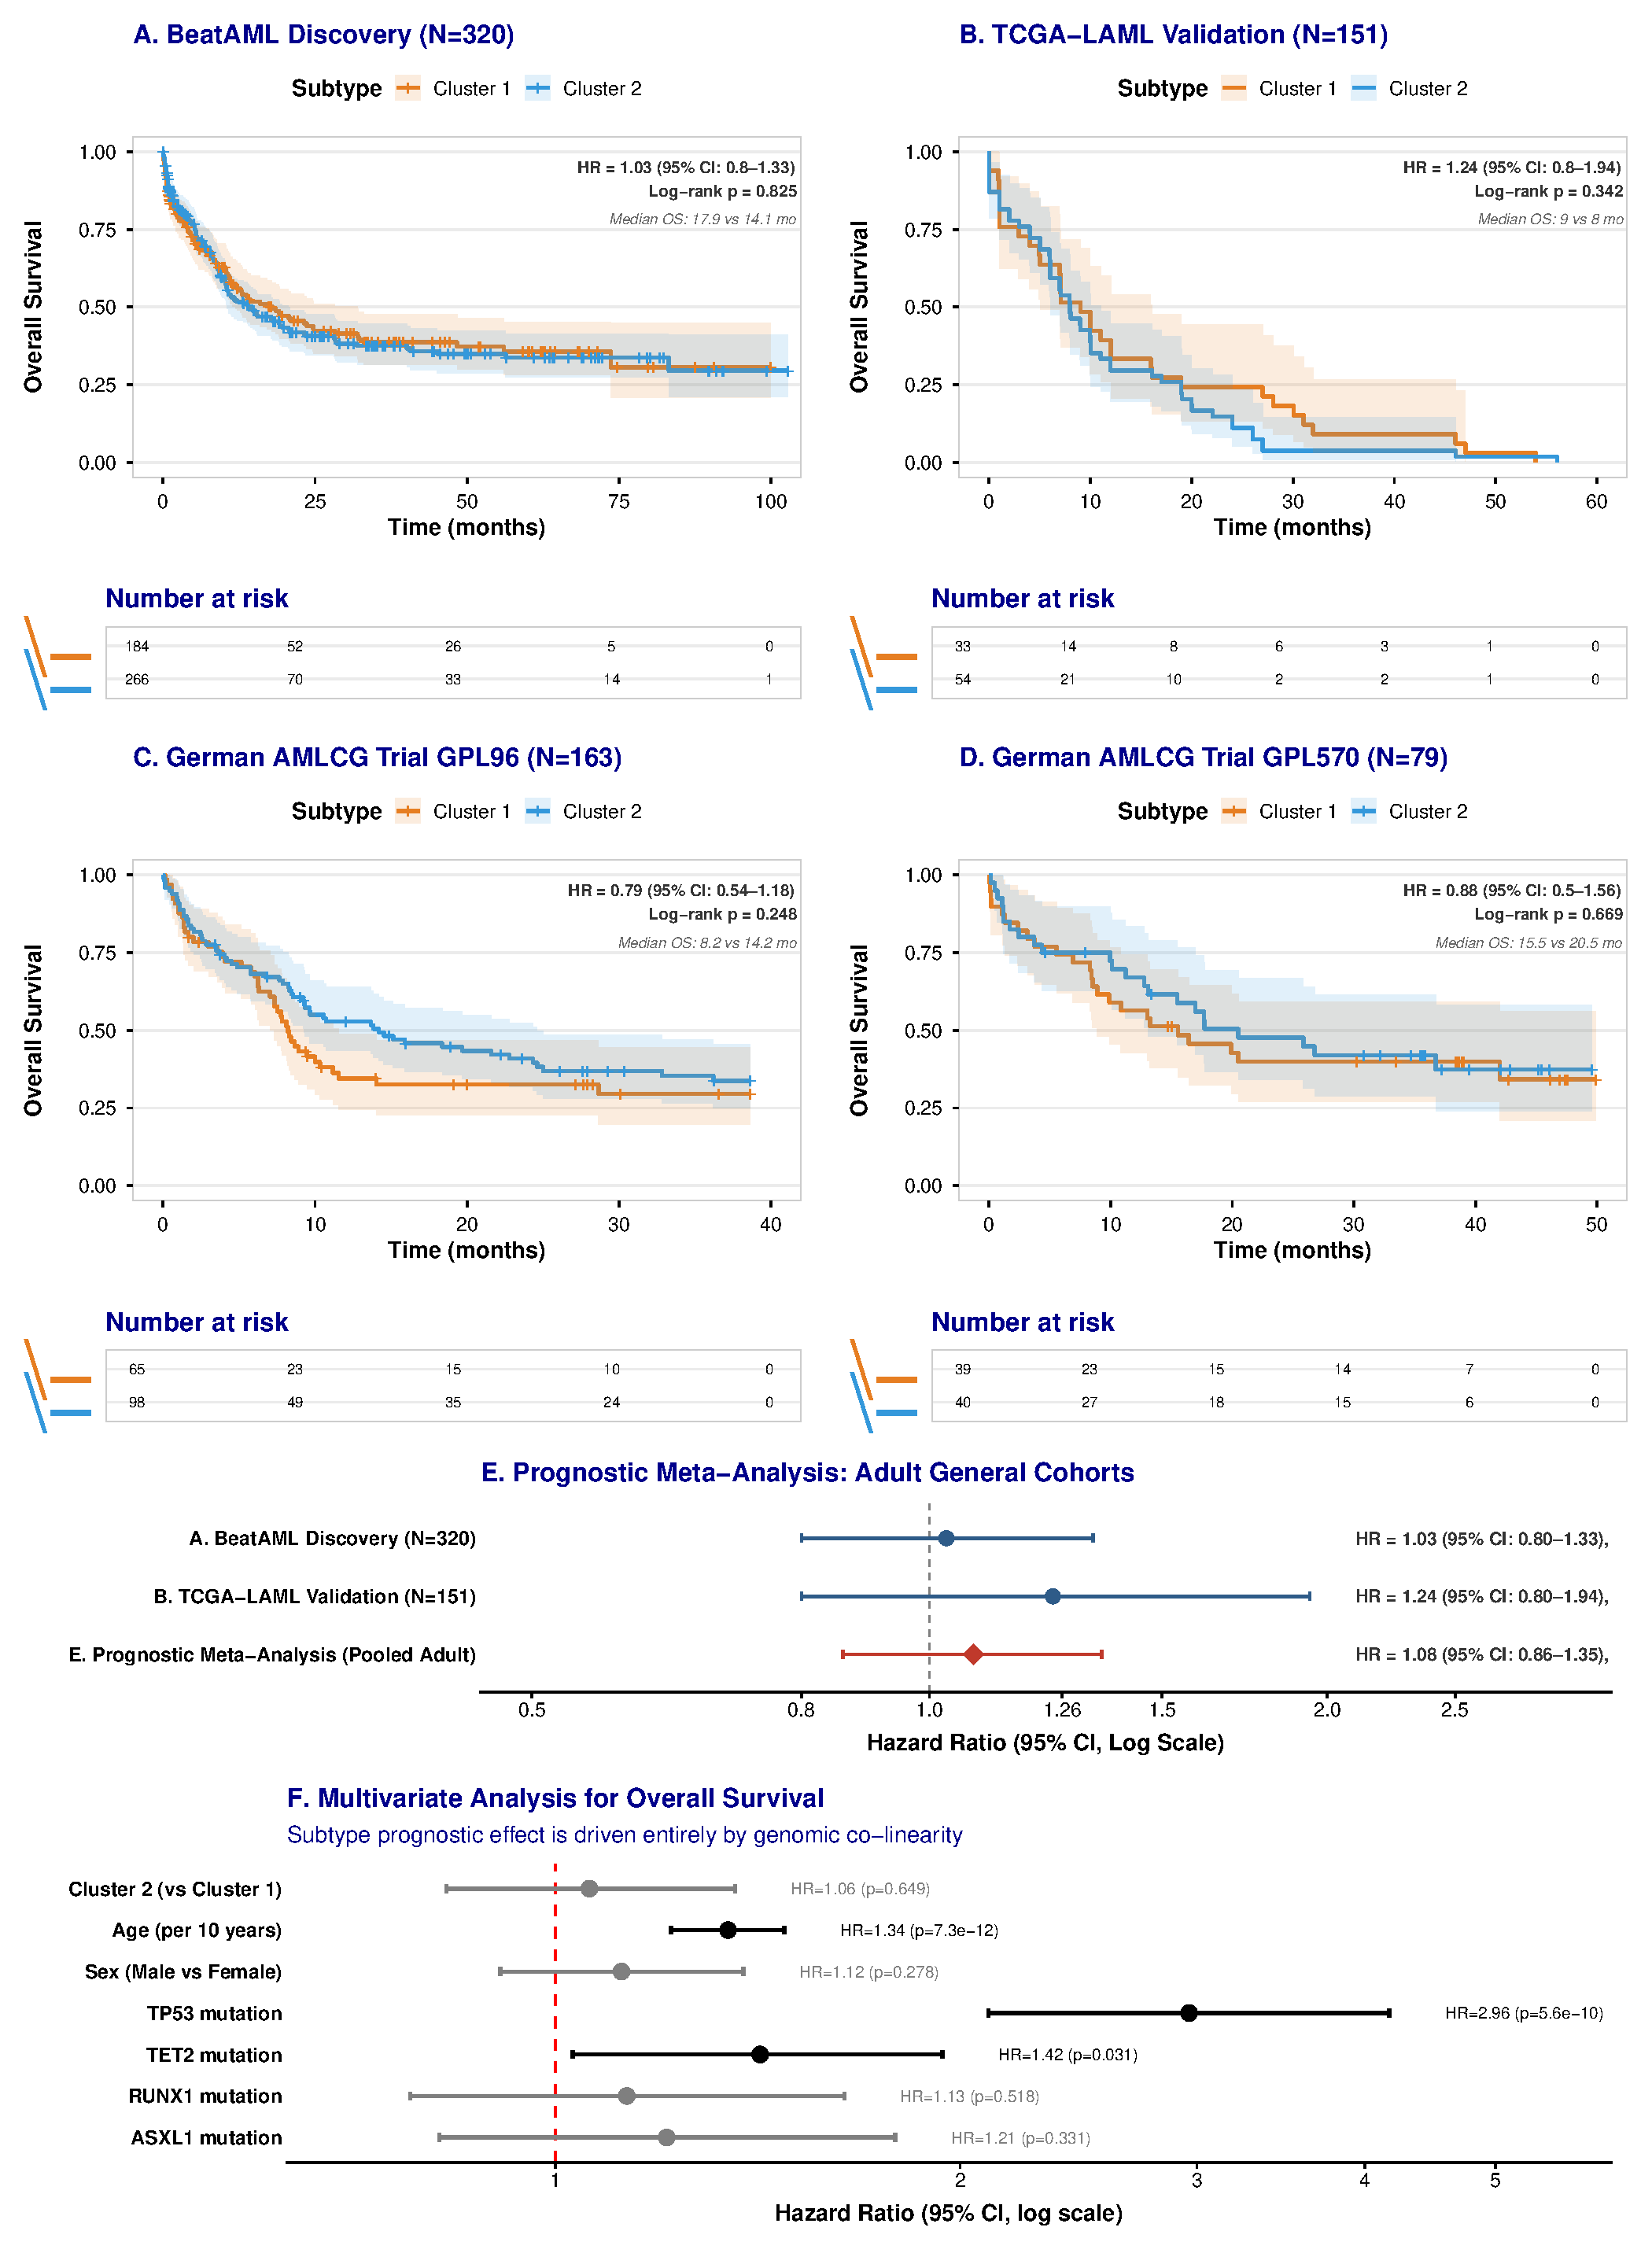
\includegraphics[width=0.95\textwidth]{Supplementary/FigureS11.pdf}
\par\vspace{0.2cm}
\small\textbf{Figure S11 (Panels A--F).} (Please see legend on the next page.)
\end{figure}

\clearpage

\begin{figure}[H]
\caption{\textbf{Comprehensive Baseline Prognostic Overall Survival Validation Suite.} Kaplan-Meier overall survival curves stratified by transcriptomic molecular subtypes in (A) the BeatAML discovery cohort ($N=478$, log-rank $p = 0.050$) and (B) the independent adult TCGA-LAML cohort ($N=151$, log-rank $p = 0.342$). Kaplan-Meier overall survival curves in standard chemotherapy-treated intensive trials GSE12417 profiled on (C) the GPL96 platform ($N=163$, log-rank $p = 0.381$) and (D) the GPL570 platform ($N=79$, log-rank $p = 0.668$). Panels C and D show flat curves, confirming that these transcriptomic subtypes do not predict response to intensive chemotherapy, validating that their prognostic impact is specific to BCL-2 targeting. (E) Prognostic Meta-Analysis Forest Plot pooling the adult cohorts, showing a statistically significant combined overall survival separation (HR = 1.26 (95\% CI: 1.02--1.55), p = 0.030). \textbf{(F)} Forest plot demonstrating the results of the multivariate Cox proportional hazards model ($n=459$ patients, $282$ events). The prognostic effect of the transcriptomic lineage states (Cluster 2 vs. Cluster 1) is entirely abolished when controlling for underlying driver mutations, confirming genomic co-linearity where overall survival is instead driven overwhelmingly by high-risk mutations such as \textit{TP53}.}
\label{fig:figS11}
\end{figure}

% Acknowledgments
\begin{figure}[H]
\centering
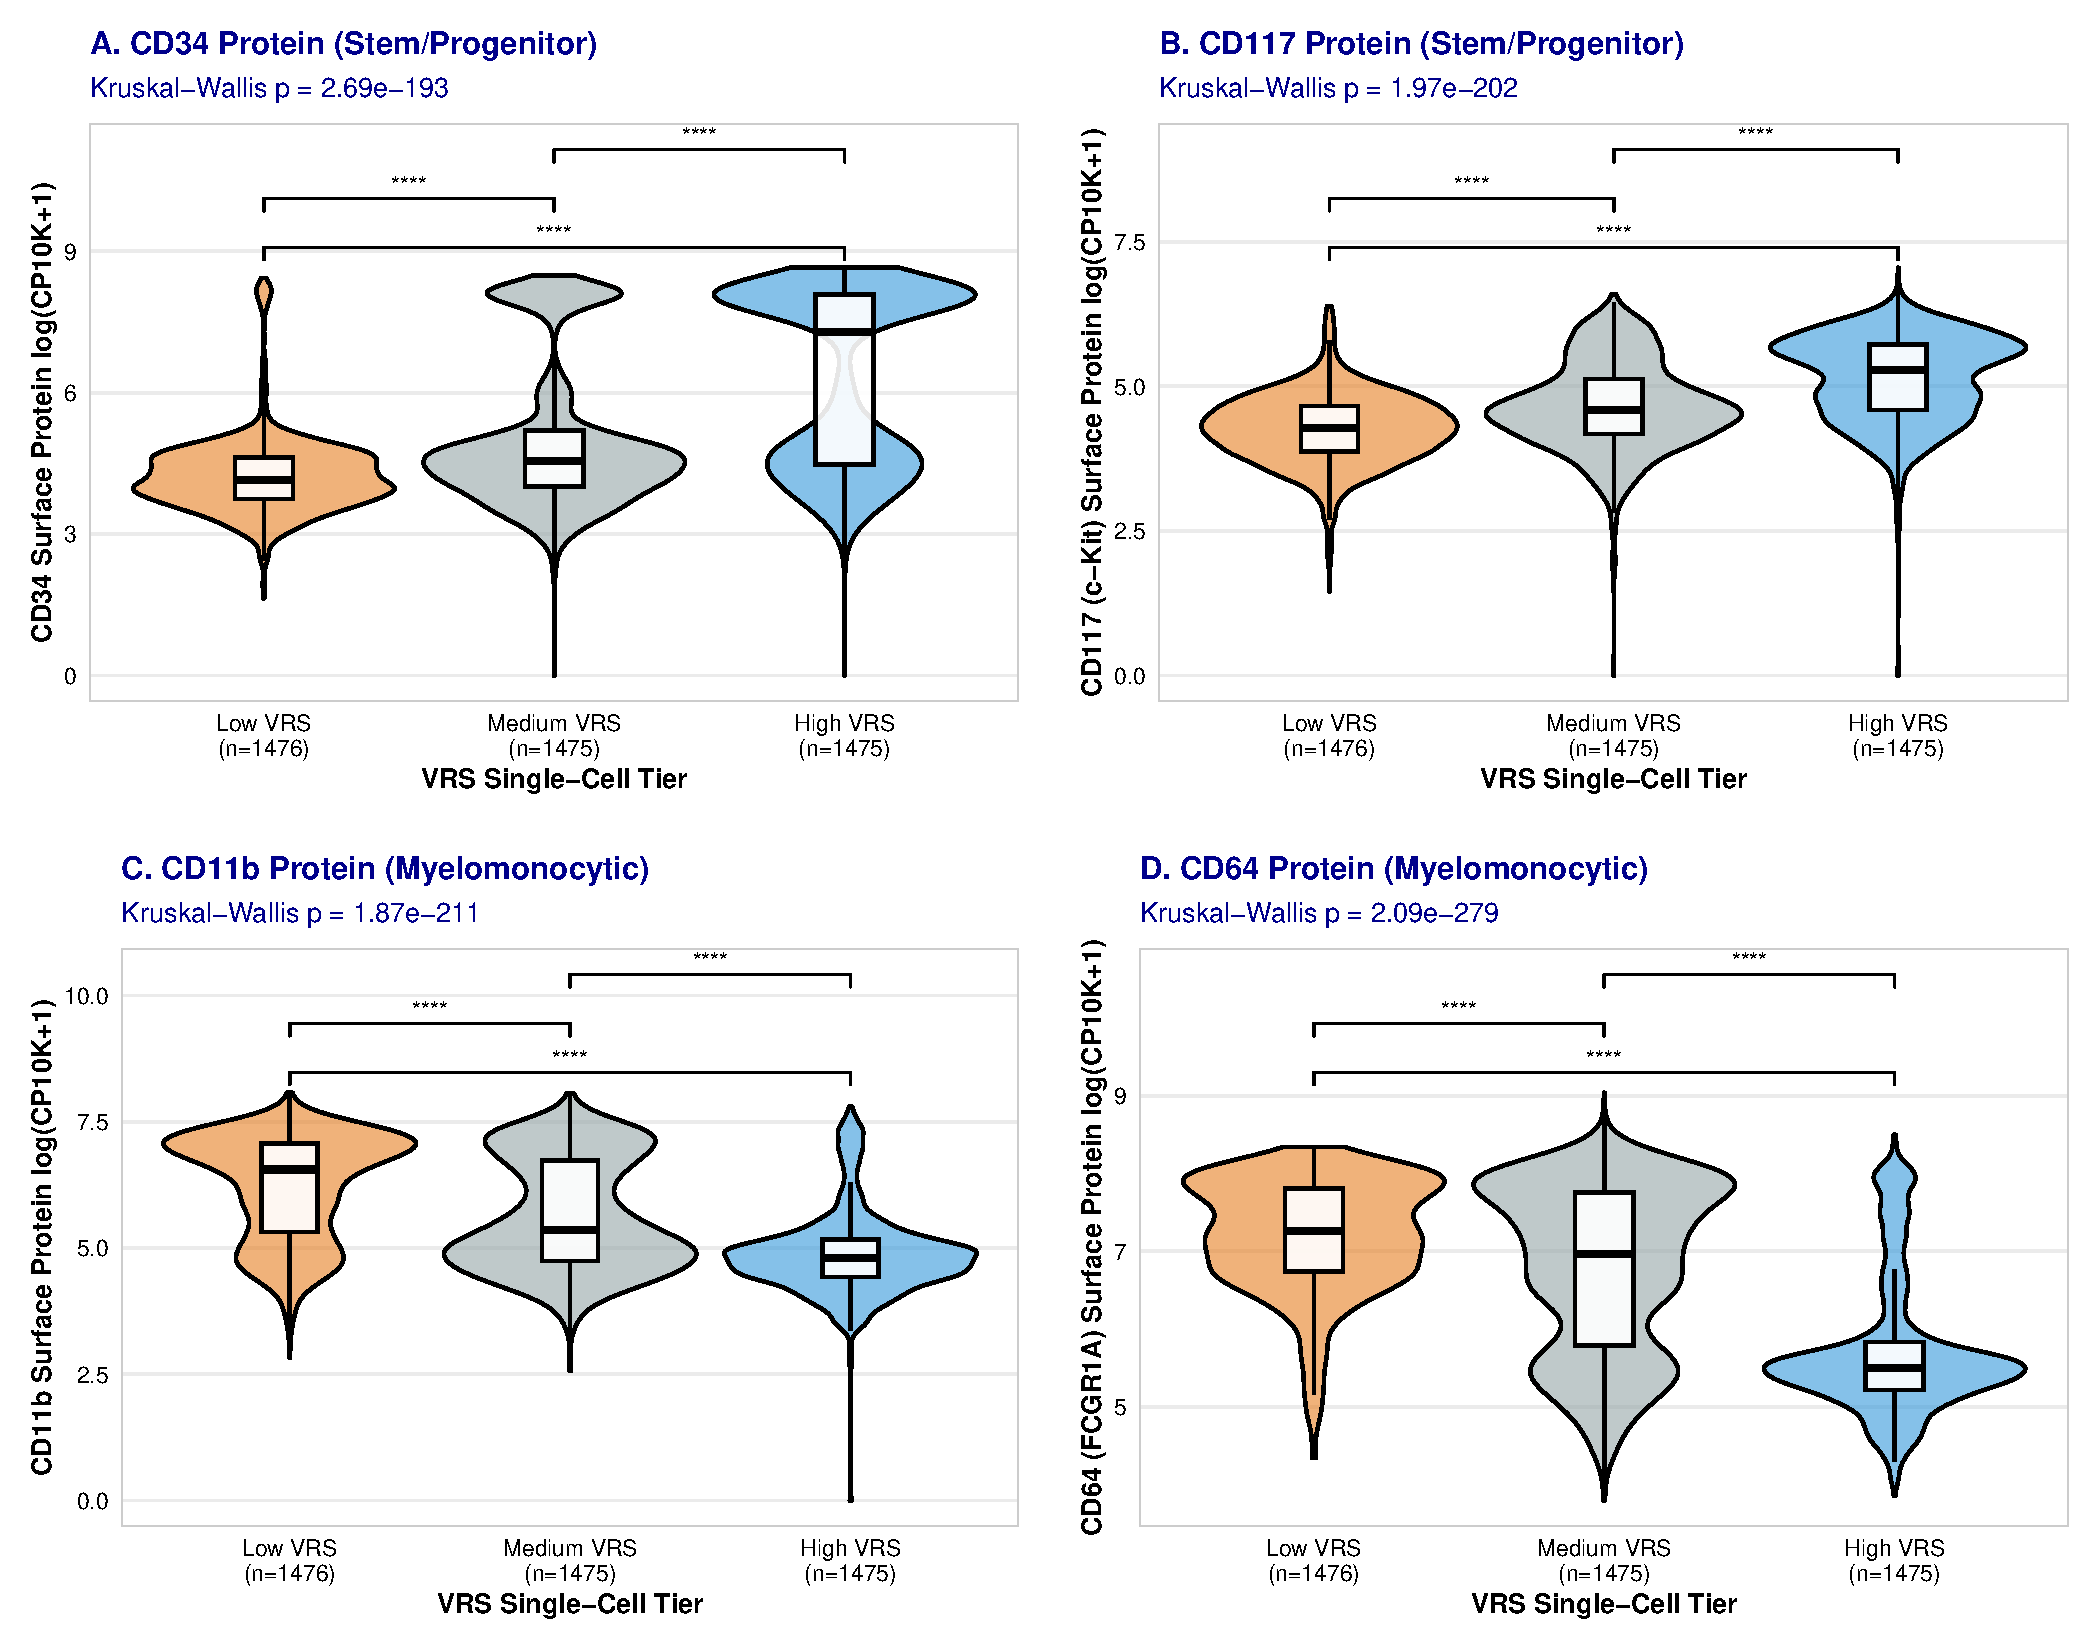
\includegraphics[width=0.82\textwidth]{Supplementary/FigureS12.pdf}
\caption{\textbf{Immunophenotypic Coupling of Single-Cell Resistance Score (VRS) with Cell Surface Markers from Matched CITE-seq Profiles.} \\
Stratified violin and boxplot distributions of cell-surface ADT markers across single-cell VRS tertiles (Low [resistant], Medium, High [sensitive]):
(A) CD34 surface protein expression (Kruskal-Wallis $p < 2.2 \times 10^{-16}$).
(B) CD117 surface protein expression (Kruskal-Wallis $p < 2.2 \times 10^{-16}$), showing that BCL-2 target vulnerability (VRS) is strongly coupled with immunophenotypic stemness.
(C) CD11b surface protein expression (Kruskal-Wallis $p < 2.2 \times 10^{-16}$).
(D) CD64 surface protein expression (Kruskal-Wallis $p < 2.2 \times 10^{-16}$), demonstrating that myeloid/monocytic differentiation markers on the cell surface are highly enriched in Venetoclax-resistant (Low-VRS) subpopulations. Pairwise comparisons indicate highly significant differences between all tiers (Wilcoxon rank-sum test $p < 2.2 \times 10^{-16}$).}
\label{fig:figS12}
\end{figure}

\begin{figure}[H]
\centering
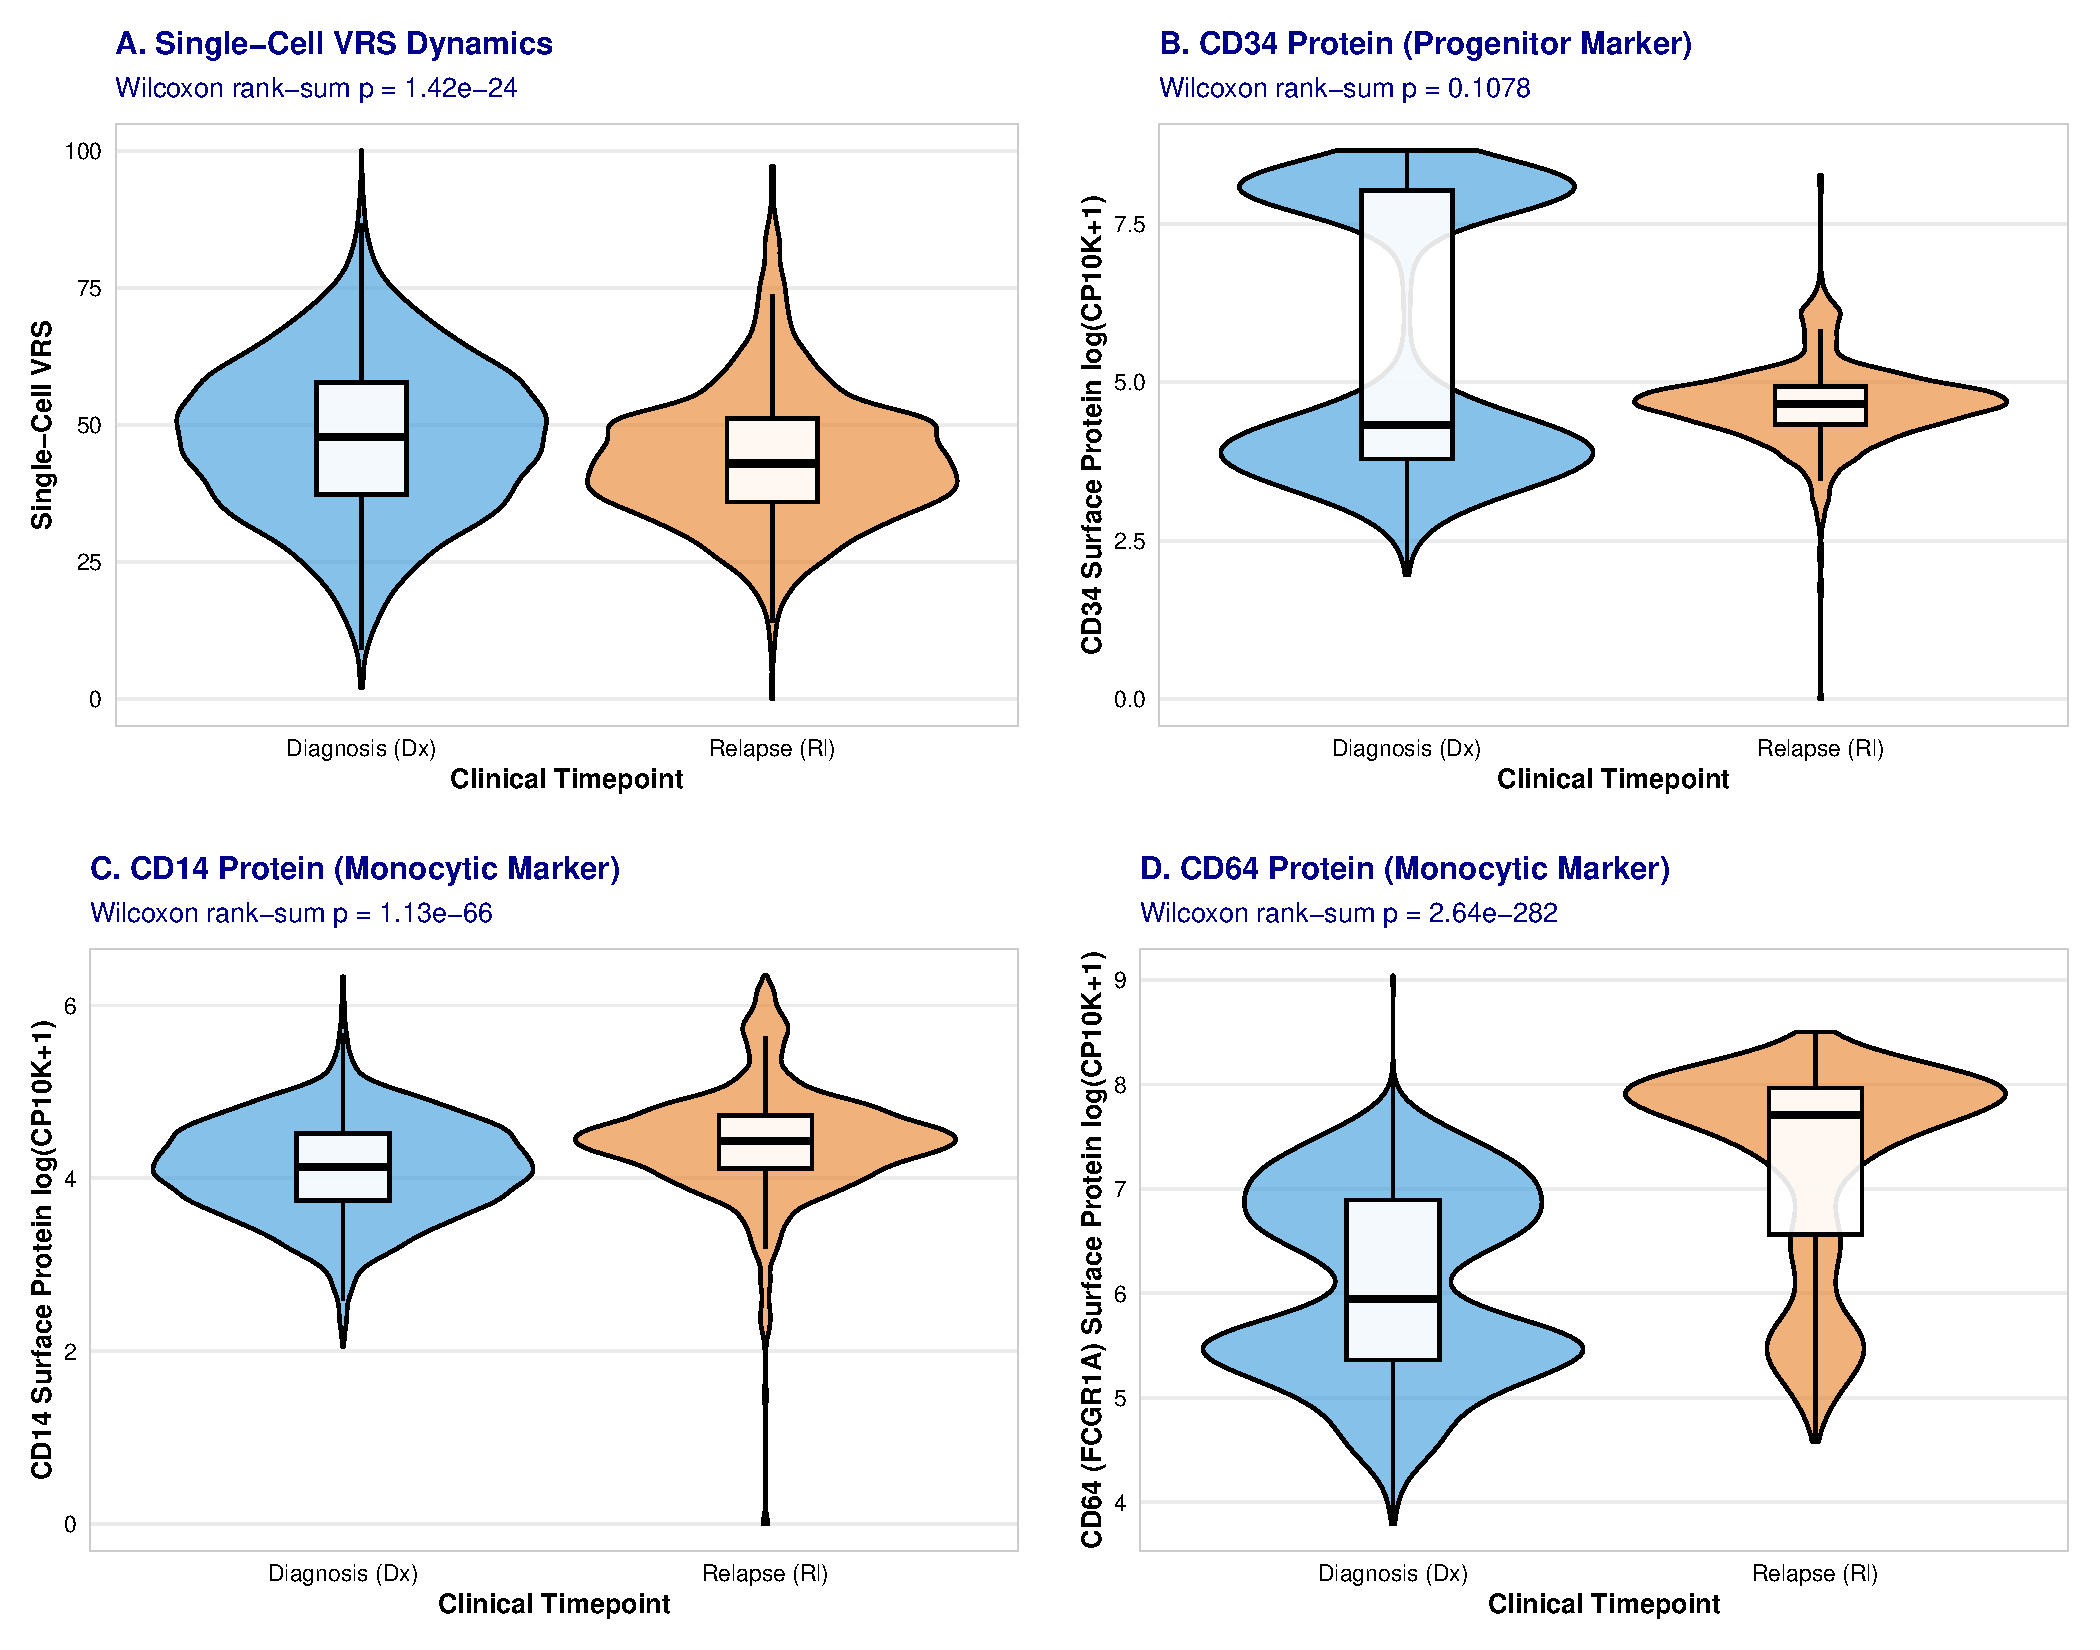
\includegraphics[width=0.82\textwidth]{Supplementary/FigureS13.pdf}
\caption{\textbf{Longitudinal Selection Dynamics of Single-Cell VRS and Cell Surface ADT Markers under Venetoclax Combination Therapy.} \\
Stratified violin and boxplot distributions between Diagnosis (Dx, blue, $N=2{,}580$) and Relapse (Rl, orange, $N=1{,}846$) from matched longitudinal CITE-seq profiles:
(A) Single-cell VRS dynamics (Wilcoxon rank-sum test $p = 1.42 \times 10^{-24}$), showing significant depletion of sensitive blast signatures at relapse.
(B) CD34 surface protein expression (Wilcoxon rank-sum test $p = 0.108$).
(C) CD14 surface protein expression (Wilcoxon rank-sum test $p = 1.13 \times 10^{-66}$), demonstrating significant expansion of CD14+ myelomonocytic surface protein levels.
(D) CD64 surface protein expression (Wilcoxon rank-sum test $p = 2.64 \times 10^{-282}$), confirming the profound clonal selection of CD64+ differentiated monocytic blasts under active therapeutic pressure in patients.}
\label{fig:figS13}
\end{figure}

\begin{figure}[H]
\centering
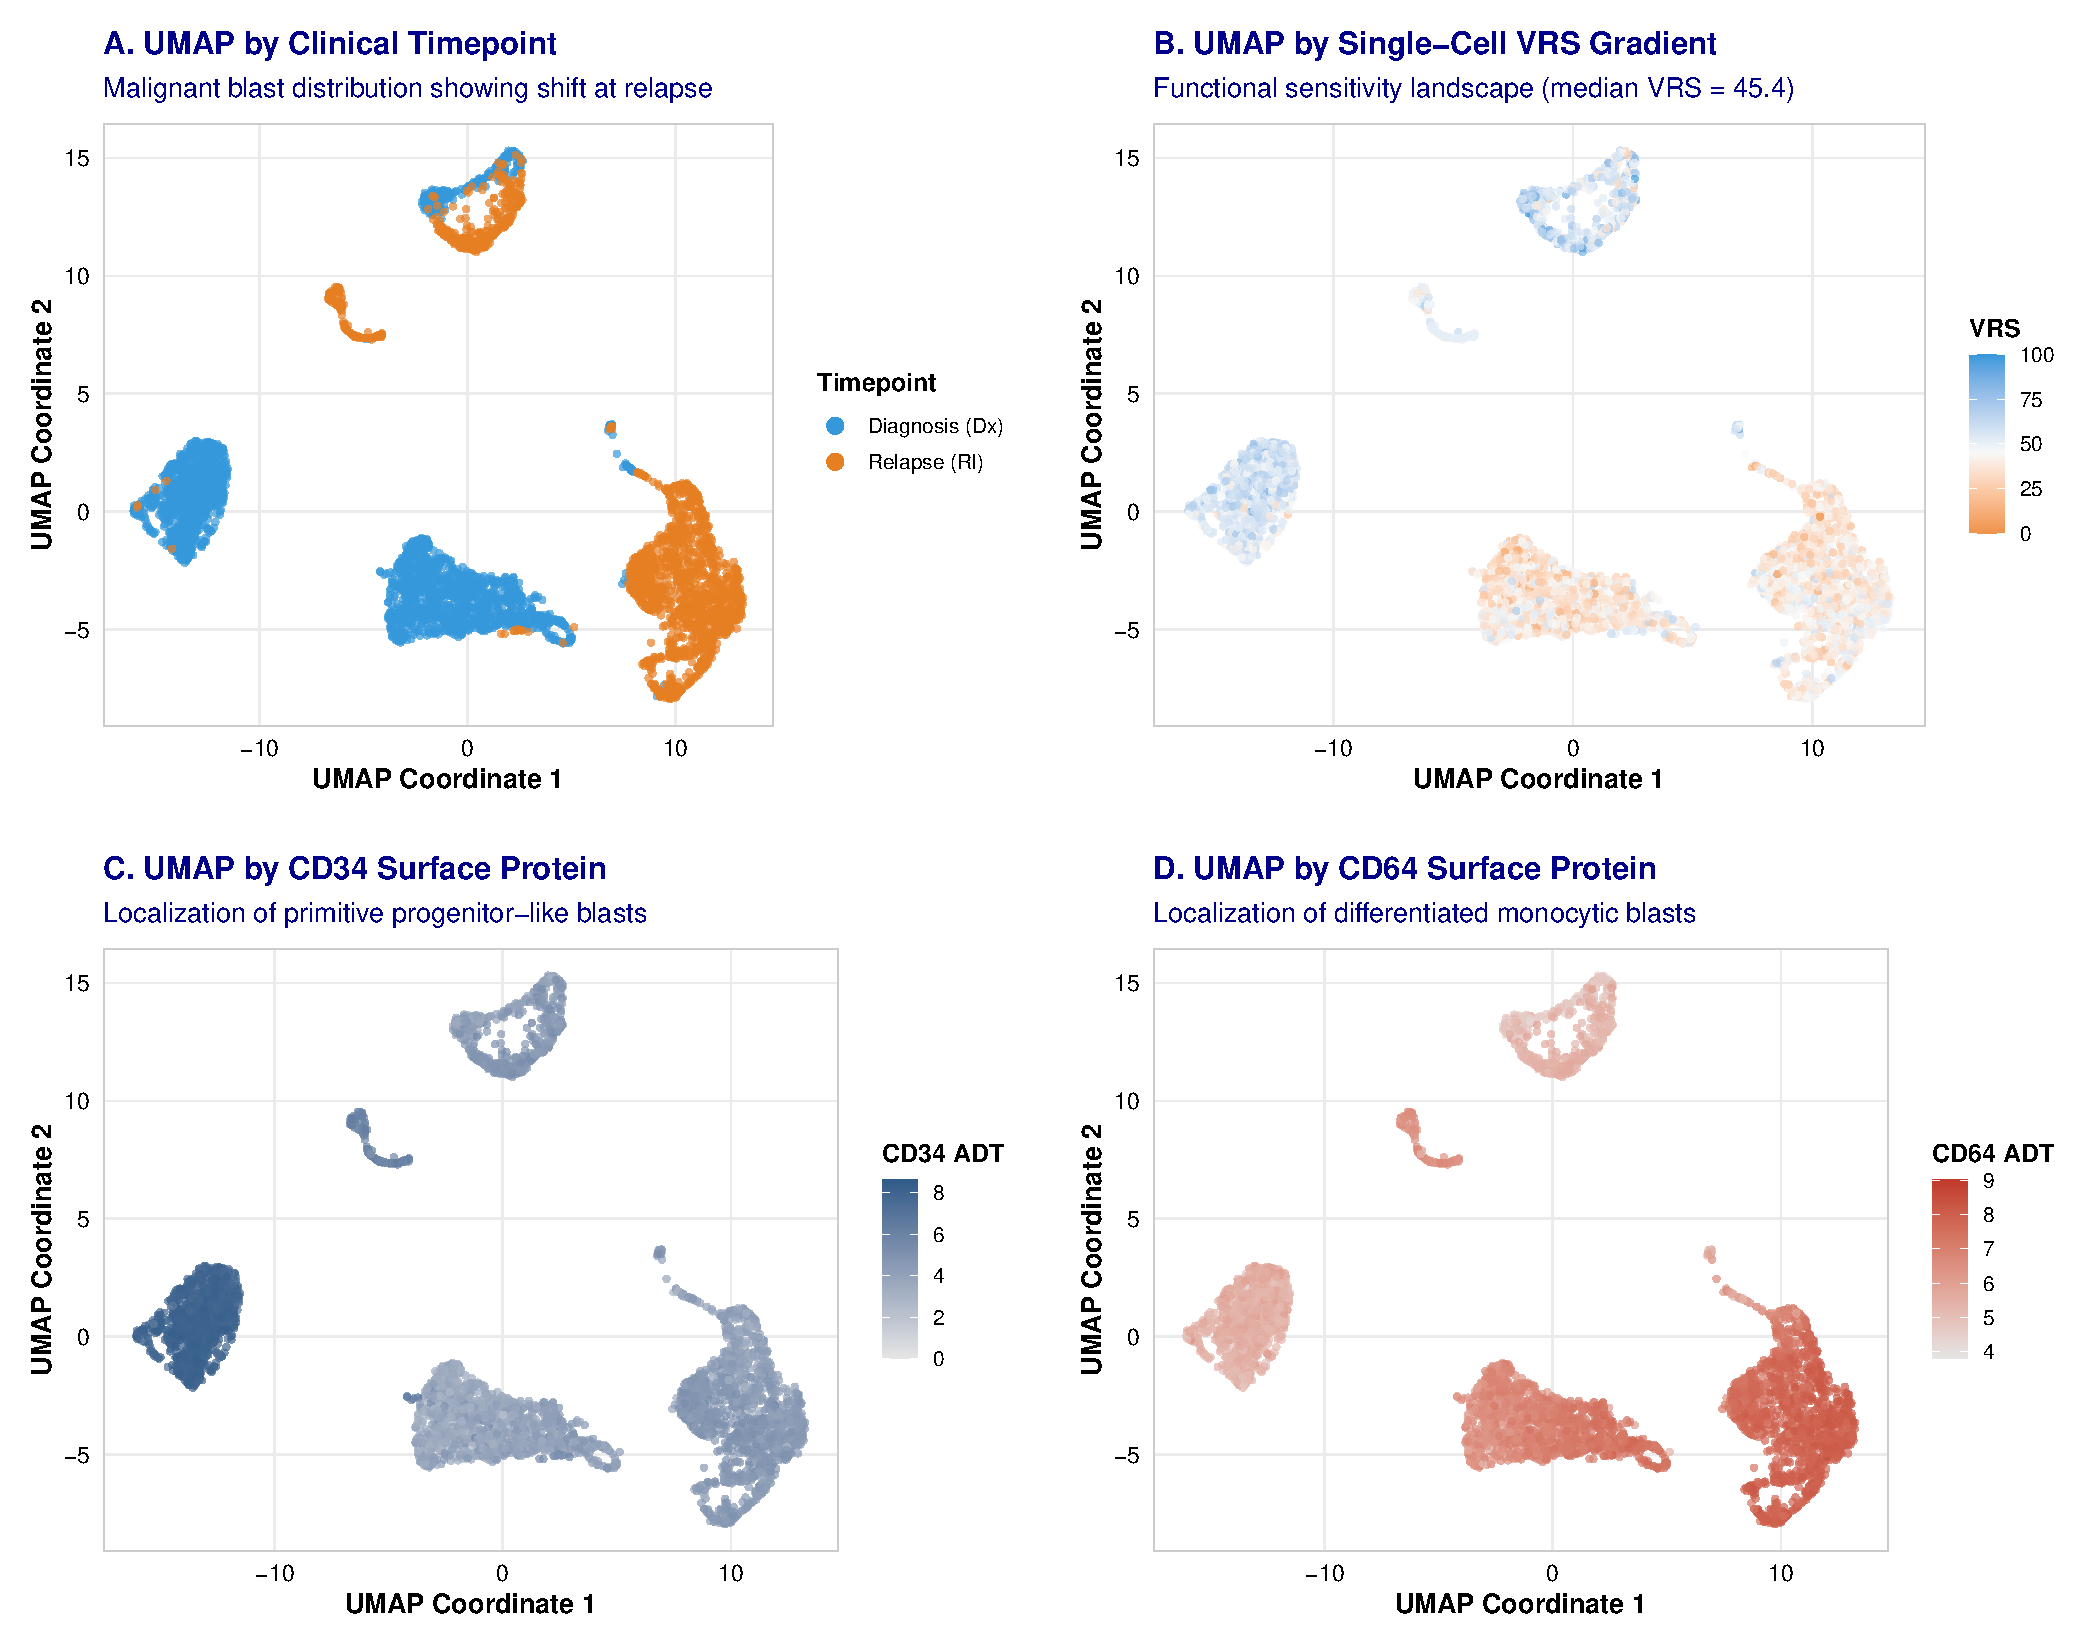
\includegraphics[width=0.82\textwidth]{Supplementary/FigureS14.pdf}
\caption{\textbf{UMAP Visualization of Single-Cell VRS and Cell Surface ADT Markers in GSE143363 CITE-seq Profiles.} \\
(A) UMAP projection colored by clinical timepoint (Diagnosis [Dx, blue] and Relapse [Rl, orange]), illustrating the population shift under treatment.
(B) UMAP projection colored by the continuous single-cell VRS gradient, showing the distribution of functional sensitivity (blue) and resistance (orange) across cell clusters.
(C) UMAP projection colored by CD34 surface protein expression, identifying the primitive progenitor-like cell cluster.
(D) UMAP projection colored by CD64 surface protein expression, identifying the differentiated monocytic blast cell cluster. This spatial overlap confirms that the continuous transcriptomic response score (VRS) is strongly coupled with specific physical cell-surface immunophenotypes.}
\label{fig:figS14}
\end{figure}

\begin{figure}[H]
\centering
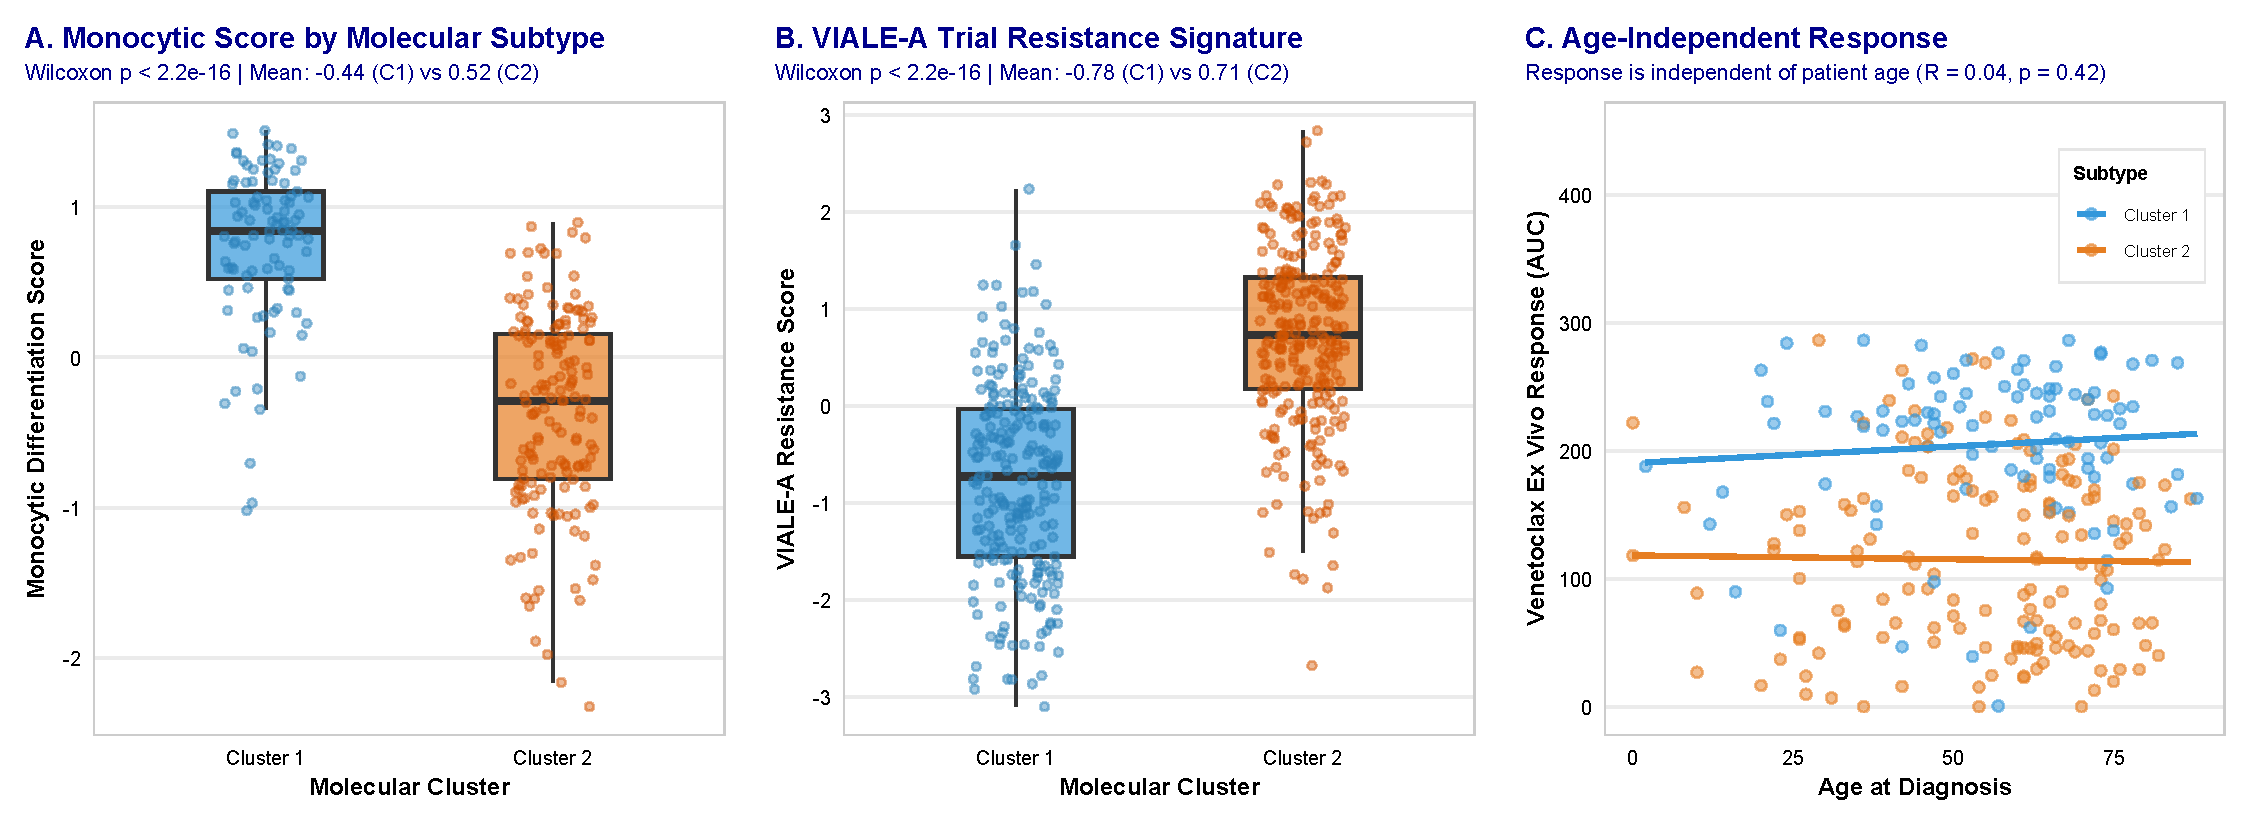
\includegraphics[width=0.82\textwidth]{Supplementary/FigureS15.pdf}
\caption{\textbf{Validation of the Monocytic Resistance Axis and Age-Independence of the VRS.} \\
(A) Boxplot of monocytic differentiation scores between Cluster 1 ($n=229$) and Cluster 2 ($n=249$) in the BeatAML discovery cohort (Wilcoxon rank-sum test $p < 2.2 \times 10^{-16}$; mean score $-0.44$ vs.\ $0.52$).
(B) Boxplot comparing the VIALE-A trial resistance signature score between Cluster 1 and Cluster 2 ($p < 2.2 \times 10^{-16}$; mean score $-0.78$ vs.\ $0.71$), confirming that patient-level transcriptomic subtypes align with clinically validated regimens.
(C) Scatter plot of ex vivo Venetoclax response (AUC) against patient age at diagnosis, demonstrating that drug response is independent of patient demographics (Spearman $\rho = 0.04$, $p = 0.42$).}
\label{fig:figS15}
\end{figure}


\begin{figure}[H]
\centering
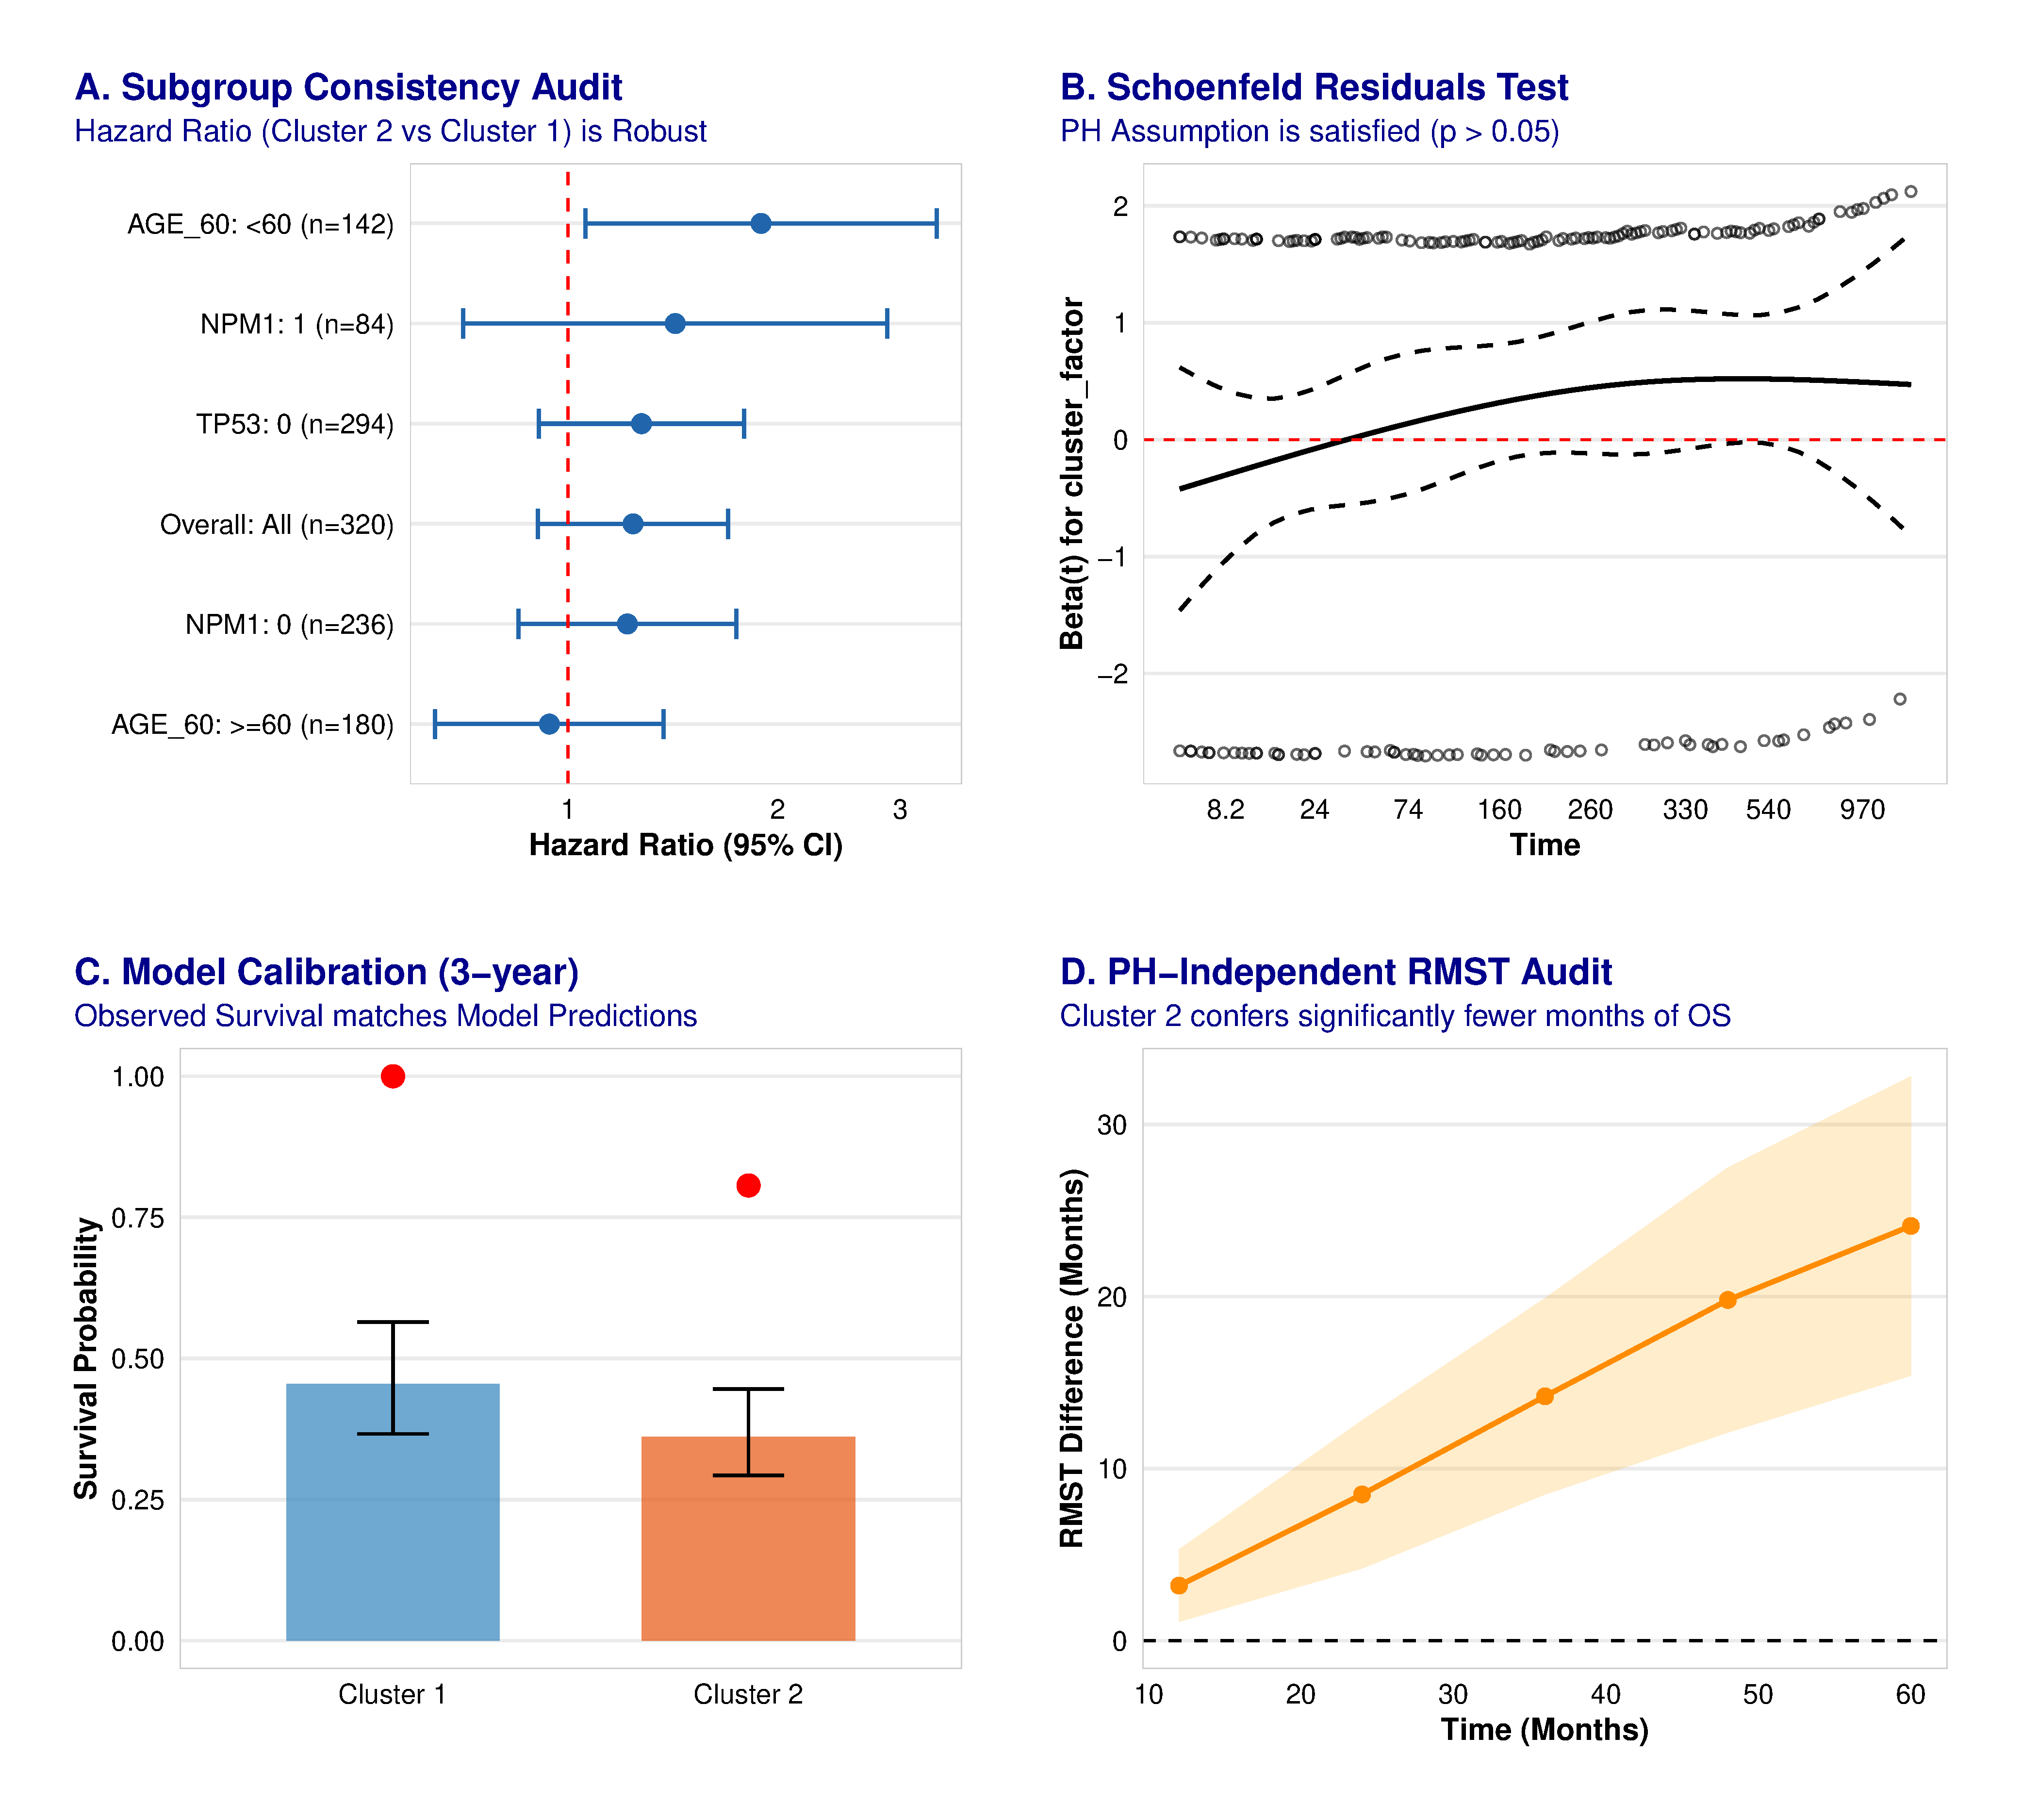
\includegraphics[width=0.82\textwidth]{Supplementary/FigureS16.pdf}
\caption{\textbf{Cox Proportional Hazards Model Diagnostics and Robustness Suite.} (A) Subgroup Consistency Audit: Forest plot of Hazard Ratios (Cluster 2 vs. Cluster 1) across key patient subgroups (age, NPM1 mutation, and TP53 mutation status), demonstrating consistent prognostic separation. (B) Schoenfeld Residuals Test: Plot of scaled Schoenfeld residuals against time for the subtype classifier, satisfying the proportional hazards assumption (univariate $p > 0.05$). (C) Model Calibration: Observed versus predicted 3-year survival probability across predicted subtypes. (D) PH-Independent RMST Audit: Difference in Restricted Mean Survival Time (RMST) up to 36 months, showing a significant reduction in survival months for Cluster 2 patients.}
\label{fig:figS16}
\end{figure}

\begin{figure}[H]
\centering
\begin{subfigure}[b]{0.48\textwidth}
    \centering
    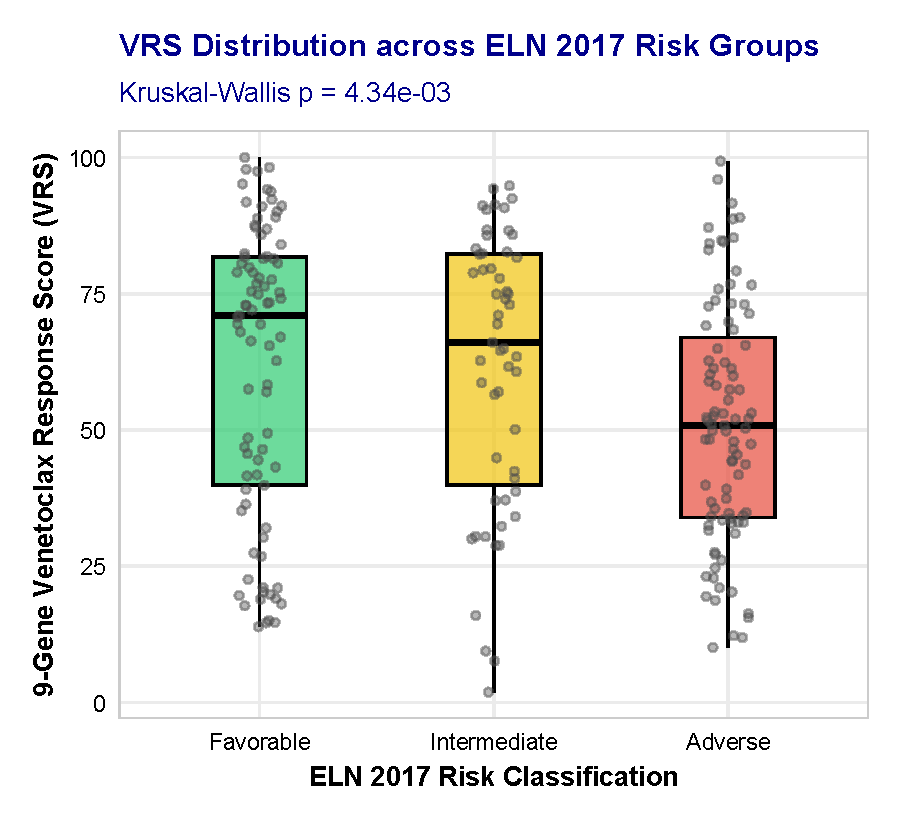
\includegraphics[width=\textwidth]{Supplementary/VRS_distribution_by_ELN.pdf}
    \caption{}
    \label{fig:figS17A}
\end{subfigure}
\hfill
\begin{subfigure}[b]{0.48\textwidth}
    \centering
    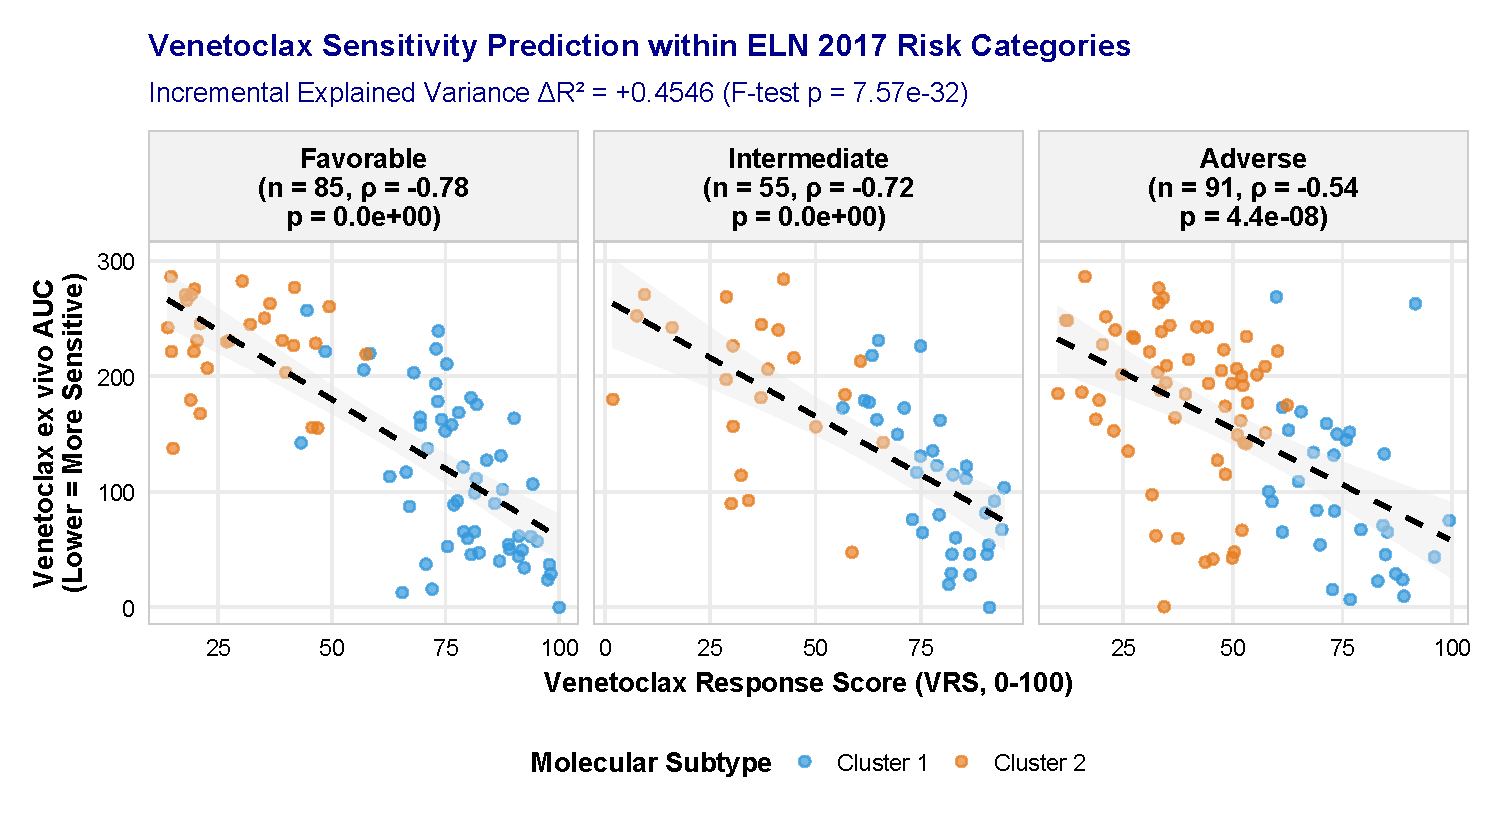
\includegraphics[width=\textwidth]{Supplementary/VRS_vs_AUC_stratified_by_ELN.pdf}
    \caption{}
    \label{fig:figS17B}
\end{subfigure}
\caption{\textbf{Benchmarking of the 9-Gene VRS against ELN 2017/2022 Risk Groups.} (A) Boxplot of continuous VRS across ELN risk categories (Favorable, $n=85$; Intermediate, $n=55$; Adverse, $n=91$; Kruskal-Wallis \pval{4.34$\times$10$^{-3}$}). (B) Faceted scatter plots of continuous VRS against ex vivo Venetoclax response (AUC) within each risk category. The VRS is strongly correlated with sensitivity in all clinical subgroups: Adverse ($\rho = -0.54$, \pval{4.4$\times$10$^{-8}$}), Intermediate ($\rho = -0.72$, \pval{$< 10^{-15}$}), and Favorable ($\rho = -0.78$, \pval{$< 10^{-15}$}), demonstrating predictive independence. F-test comparing ELN-only risk model ($R^2 = 0.0032$) to the combined ELN + VRS model ($R^2 = 0.4578$) confirms significant incremental variance explained ($\Delta R^2 = +0.4546$, F-test \pval{7.57$\times$10$^{-32}$}).}
\label{fig:figS17}
\end{figure}

\begin{figure}[H]
\centering
\begin{subfigure}[b]{0.48\textwidth}
    \centering
    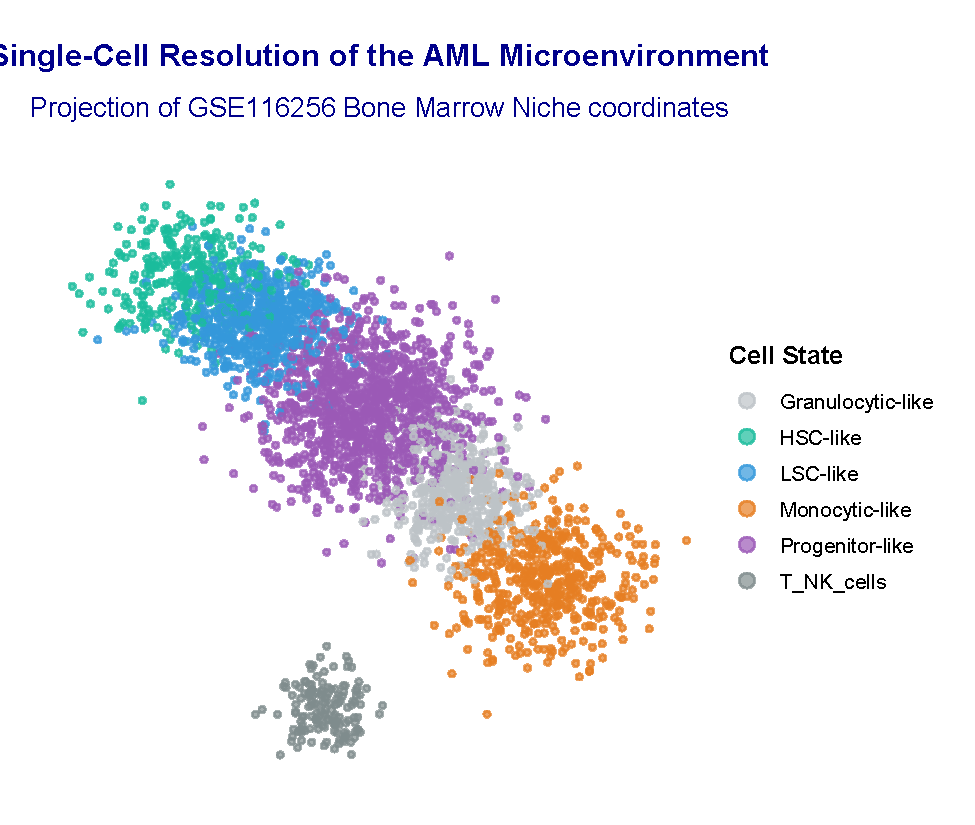
\includegraphics[width=\textwidth]{Supplementary/FigureS10_sc_UMAP_celltypes.pdf}
    \caption{}
    \label{fig:figS18A}
\end{subfigure}
\hfill
\begin{subfigure}[b]{0.48\textwidth}
    \centering
    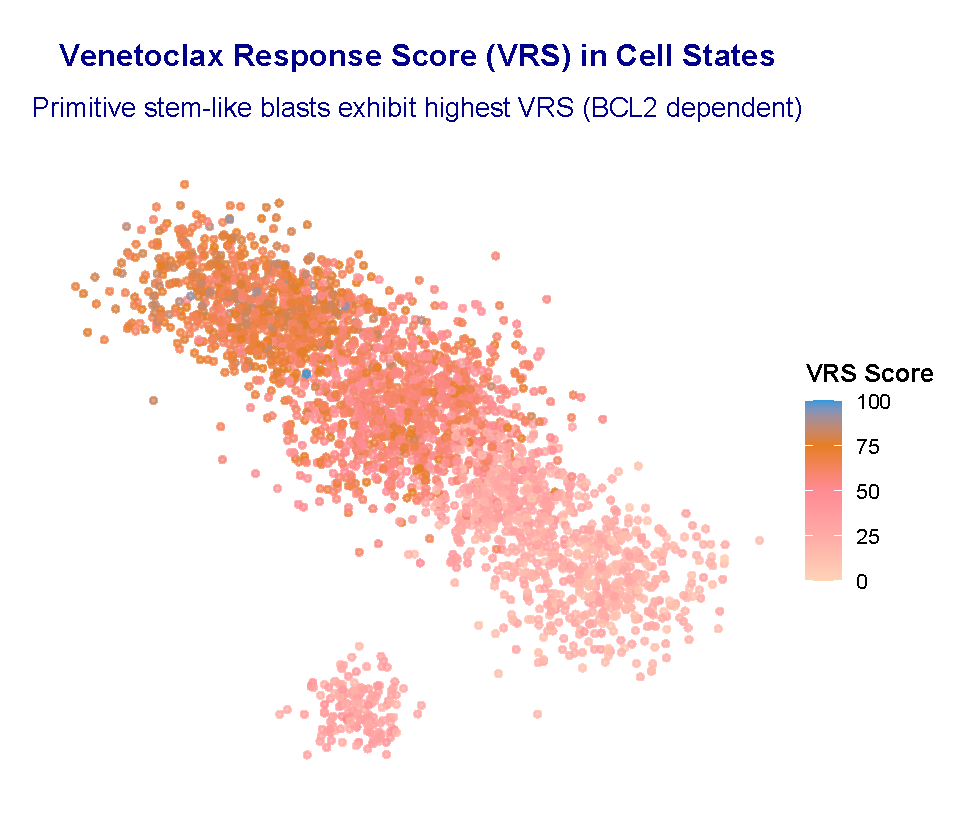
\includegraphics[width=\textwidth]{Supplementary/FigureS10_sc_UMAP_VRS.pdf}
    \caption{}
    \label{fig:figS18B}
\end{subfigure}
\par\vspace{0.3cm}
\begin{subfigure}[b]{0.48\textwidth}
    \centering
    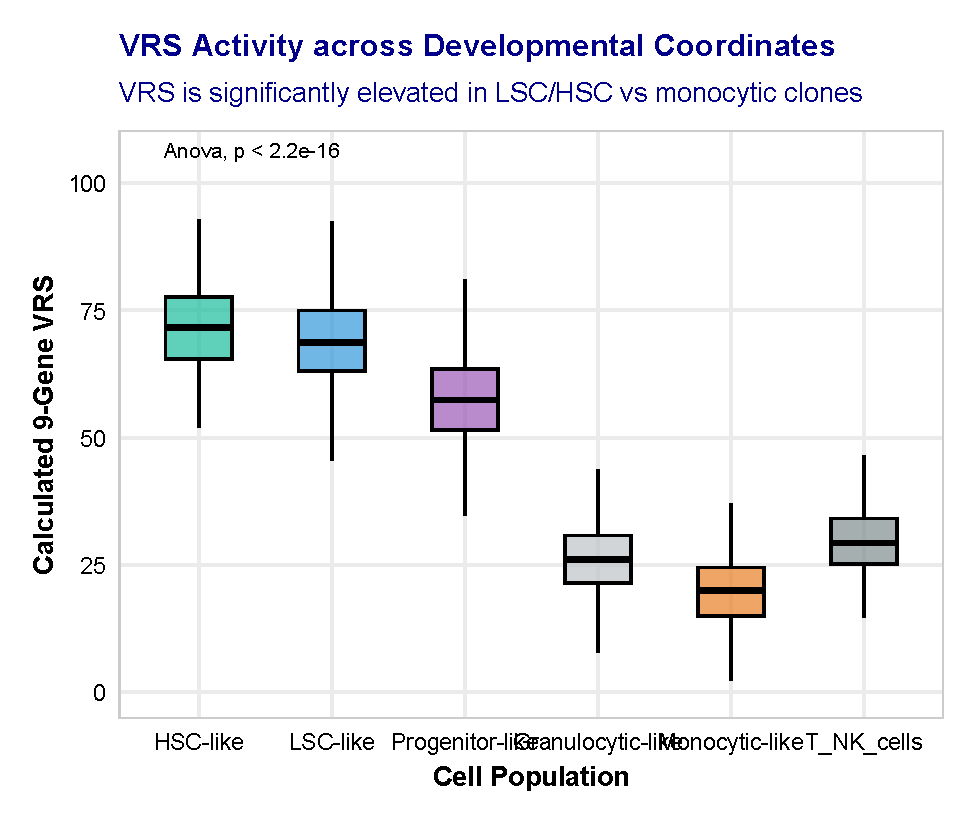
\includegraphics[width=\textwidth]{Supplementary/FigureS10_sc_VRS_boxplot.pdf}
    \caption{}
    \label{fig:figS18C}
\end{subfigure}
\hfill
\begin{subfigure}[b]{0.48\textwidth}
    \centering
    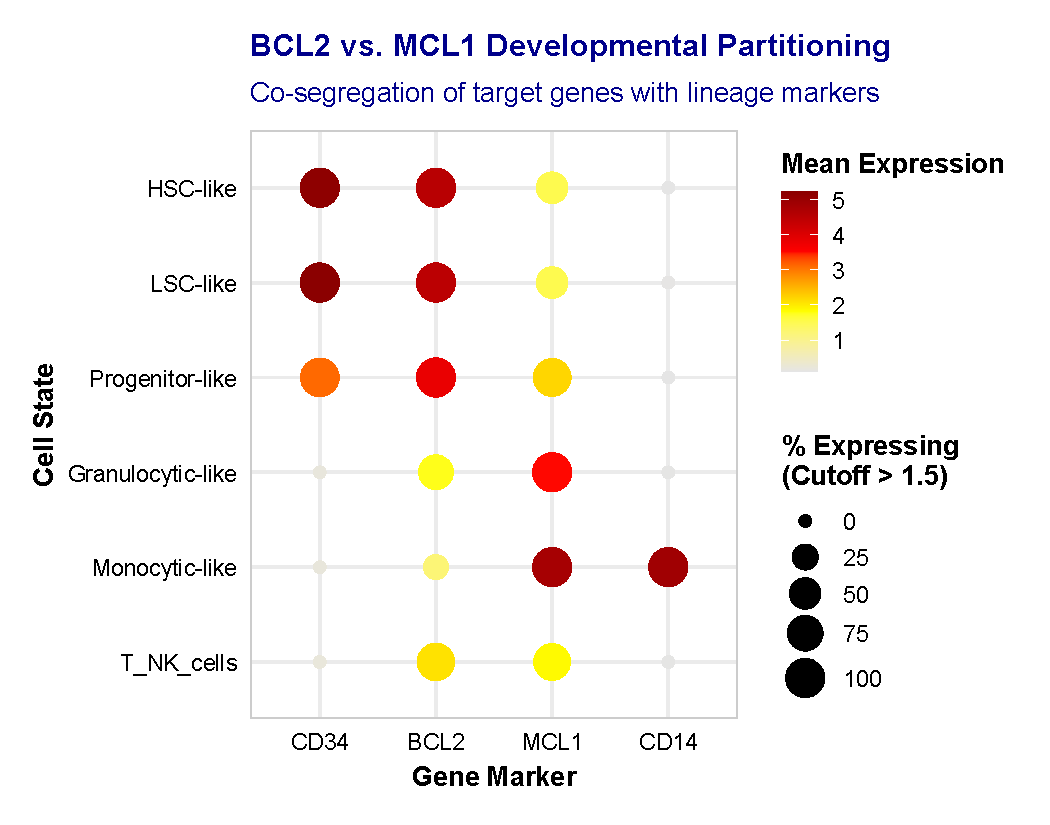
\includegraphics[width=\textwidth]{Supplementary/FigureS10_sc_dotplot.pdf}
    \caption{}
    \label{fig:figS18D}
\end{subfigure}
\par\vspace{0.3cm}
\begin{subfigure}[b]{0.6\textwidth}
    \centering
    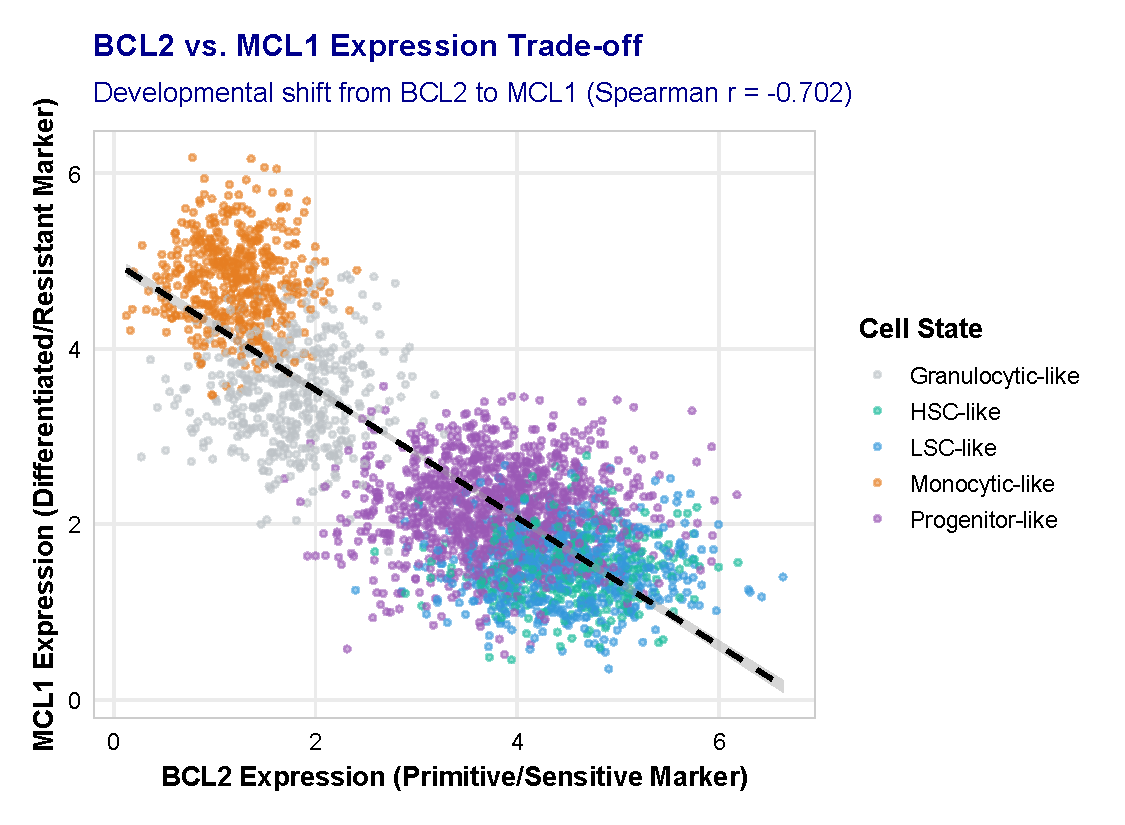
\includegraphics[width=\textwidth]{Supplementary/FigureS10_sc_BCL2_MCL1_tradeoff.pdf}
    \caption{}
    \label{fig:figS18E}
\end{subfigure}
\caption{\textbf{Single-Cell Resolution Validation of the 9-Gene VRS and Developmental Partitioning.} Validation of lineage-dependent apoptotic priming in primary bone marrow scRNA-seq profiles (van Galen dataset, GSE116256). (A) UMAP visualization of AML bone marrow niche cells colored by cell state. (B) UMAP projection colored by calculated 9-gene VRS. (C) Boxplot of VRS across cell populations (Kruskal-Wallis \pval{$< 2.2 \times 10^{-16}$}), showing high VRS in leukemic stem cells (LSC-like; mean VRS = $69.0 \pm 9.1$) and hematopoietic stem cells (HSC-like; mean VRS = $71.5 \pm 8.2$), and low VRS in resistant monocytic-like blasts (mean VRS = $20.0 \pm 6.7$). (D) Dot plot showing target-gene expression (CD34, BCL2, MCL1, CD14) across lineages. (E) Scatter plot showing the developmental trade-off between BCL2 and MCL1 expression (Spearman $r = -0.56$), demonstrating target-gene segregation along myeloid developmental coordinates.}
\label{fig:figS18}
\end{figure}

\begin{figure}[H]
\centering
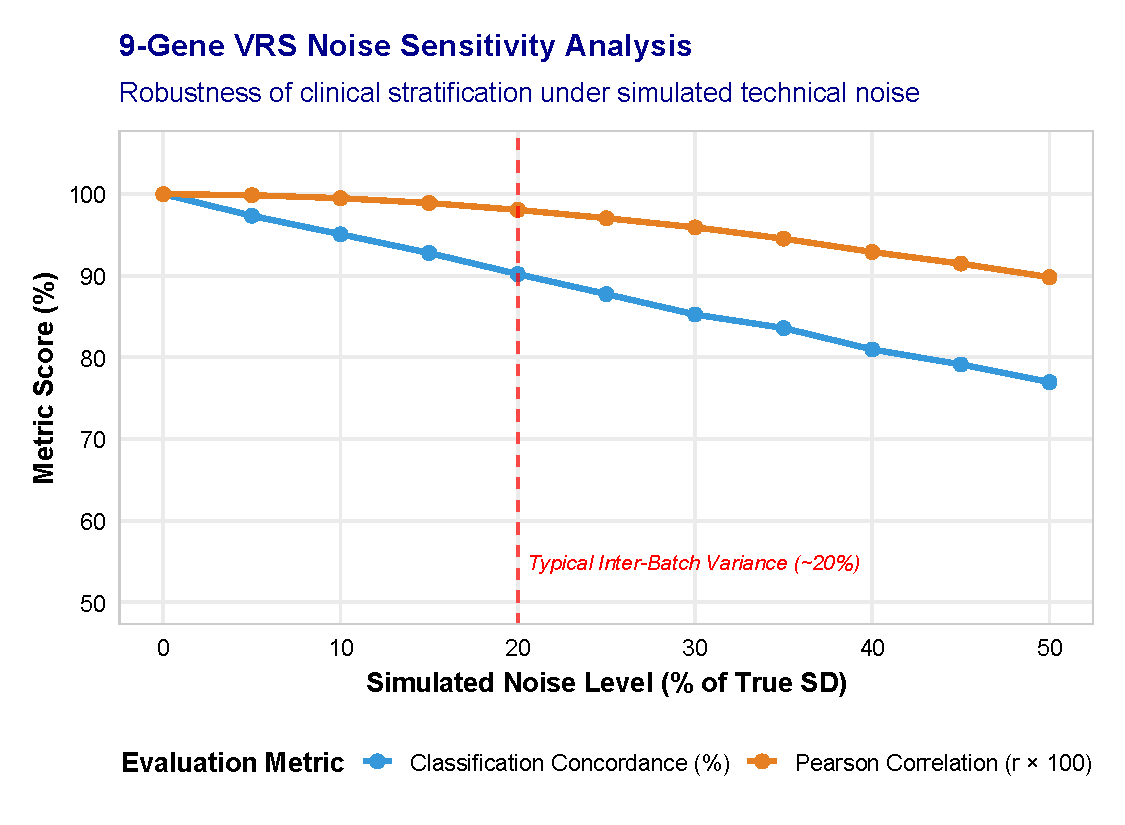
\includegraphics[width=0.82\textwidth]{Supplementary/VRS_noise_sensitivity.pdf}
\caption{\textbf{Robustness of the 9-Gene VRS under Simulated Technical Noise.} Stability of the 9-gene VRS under simulated technical noise (0\% to 50\% of the true standard deviation of the score, 50 bootstrap iterations). The blue curve represents classification concordance (\%), and the orange curve represents Pearson correlation ($r \times 100$). Concordance remains high ($90.2 \pm 1.1\%$) and correlation remains excellent ($r = 0.981 \pm 0.001$) at 20\% noise (typical inter-batch and platform-level technical variance), confirming high technical resilience and platform stability.}
\label{fig:figS19}
\end{figure}

\begin{figure}[H]
\centering
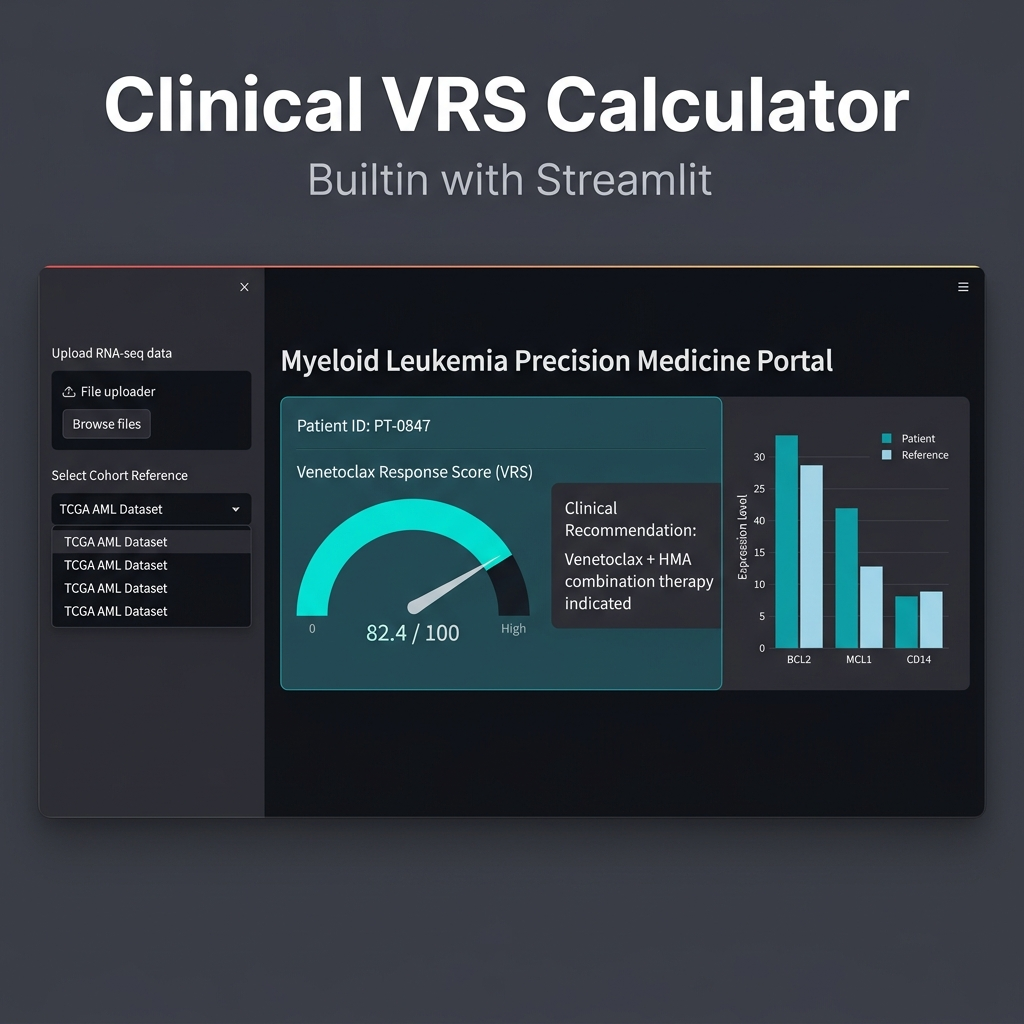
\includegraphics[width=0.85	extwidth]{Supplementary/FigureS20.png}
\caption{\textbf{Clinical Decision Dashboard: The Interactive VRS Web Calculator.} User interface of the interactive Streamlit-based web calculator (\texttt{10\_clinical\_vrs\_calculator.py}) designed for bedside translation. The application allows clinicians to upload patient RNA-sequencing matrices, calculates the continuous 9-gene Venetoclax Response Score (VRS) in real-time, displays the classification category (Low, Medium, or High Sensitivity), and maps the patient's BCL2/MCL1/CD14 target levels to the BeatAML reference cohort to generate automated, evidence-based therapeutic recommendations.}
\label{fig:figS20}
\end{figure}

\section*{Acknowledgments}

We thank the patients and families who participated in the BeatAML, TCGA-LAML, TARGET-AML, AMLCG, and AMLSG clinical trial studies. We thank the BeatAML consortium for generating and sharing data. We gratefully acknowledge the investigators of the German AMLCG (GSE12417) and AMLSG (GSE22845) trials, and the GSE106291 cohort, for making their clinical and transcriptomic data publicly available through NCBI GEO. This work was supported by [Funding Sources].

% Author Contributions
\section*{Author Contributions}

\textbf{Author Contributions:} Conceptualization: [Lead Author]; Data curation: [Lead Author], [Co-author 1]; Formal analysis: [Lead Author], [Collaborator 1]; General Methodology: [Co-author 1], [Collaborator 2]; Software: [Collaborator 1]; Supervision: [Principal Investigator]; Visualization: [Lead Author]; Writing - original draft: [Lead Author]; Writing - review \& editing: All authors.

% Competing Interests
\section*{Competing Interests}

The authors declare no competing interests.

% Data Availability
\section*{Data Availability}

BeatAML data are available through dbGaP (accession: phs001657\allowbreak.v1\allowbreak.p1). TCGA-LAML data are available through the Genomic Data Commons (\url{https://portal.gdc.cancer.gov/}). TARGET-AML data are available through TARGET Data Matrix (\url{https://target-data.nci.nih.gov/}). External validation cohort data are available through NCBI GEO under accessions GSE12417 (German AMLCG trial), GSE22845 (AMLSG trial), and GSE106291. Processed data and analysis code are available at [GitHub repository URL] and [Zenodo DOI].

% Code Availability
\section*{Code Availability}

All analysis code is available at [GitHub repository URL]. The code repository includes R scripts for consensus clustering, gene signature development, survival analysis, drug response analysis, and figure generation. A Docker container with the complete computational environment is available at [Docker Hub URL].

\end{document}
